\documentclass[a4paper,12pt]{book}

\usepackage{tikz}
\usetikzlibrary{positioning}
\usepackage{float}
\usepackage[french]{babel}

% mise en page des tableaux
\usepackage{array}
\usepackage{tabularx}
\usepackage[table,xcdraw]{xcolor}
\usepackage{wrapfig}
\usepackage{pdfpages}
\usepackage{pifont}
\usepackage{enumitem}
\usepackage{subcaption}
\usepackage{color, colortbl}
\definecolor{Gray}{gray}{0.9}
\definecolor{LightCyan}{rgb}{0.88,1,1}
\definecolor{babyblue}{rgb}{0.54, 0.81, 0.94}
\definecolor{ao(english)}{rgb}{0.0, 0.5, 0.0}
\definecolor{bittersweet}{rgb}{1.0, 0.44, 0.37}
\usepackage{longtable}
\usepackage{multirow}
\usepackage{lscape}
\usepackage{afterpage}
\usepackage{rotating}
\usepackage[nottoc,notlof,notlot]{tocbibind}
\usepackage{tocloft}
\setlength{\cftchapnumwidth}{3em}
\setlength{\cftsecnumwidth}{3em}
\setlength{\cftsubsecnumwidth}{4em}
\setlength{\cftsubsubsecnumwidth}{4em}

\graphicspath{{images/}{diagrammes/}{captures/}}
\newlength\figureheight
\newlength\figurewidth
\usepackage{ifthen}
\usepackage{ifpdf}
\usepackage[hyphens]{url}
\usepackage{ragged2e}
\ifpdf
\usepackage[unicode]{hyperref}
\else
\usepackage{hyperref}
\fi
\hypersetup{%
colorlinks=true,
linkcolor=black,
citecolor=black,
urlcolor=blue}

\usepackage[top=2.5cm,bottom=2.5cm,right=2.5cm,left=2.5cm]{geometry}
\usepackage{changepage}

\newcolumntype{L}{>{\raggedright\arraybackslash}X}
\newcolumntype{Y}{>{\RaggedRight\arraybackslash}X}
\newcolumntype{c}[1]{>{\centering\let\newline\\\arraybackslash\hspace{0pt}}m{#1}}
\newcolumntype{l}[1]{>{\raggedright\let\newline\\\arraybackslash\hspace{0pt}}m{#1}}
\newcolumntype{r}[1]{>{\raggedleft\let\newline\\\arraybackslash\hspace{0pt}}m{#1}}

\usepackage{xltabular}
\renewcommand{\tablename}{Tableau}
\renewcommand{\figurename}{Figure}
\raggedbottom
\usepackage{placeins}

% références bibliographiques (natbib, cohérent avec bibliography.bib existant)
\usepackage[round]{natbib}

% extraits de code (manifestes YAML, Java) — ajouté pour les chapitres de réalisation
\usepackage{listings}
\lstdefinestyle{codestyle}{
    backgroundcolor=\color{Gray!30},
    basicstyle=\ttfamily\footnotesize,
    keywordstyle=\color{blue},
    commentstyle=\color{ao(english)},
    stringstyle=\color{bittersweet},
    numbers=left,
    numberstyle=\tiny\color{gray},
    breaklines=true,
    breakatwhitespace=false,
    frame=single,
    tabsize=2,
    showstringspaces=false
}
\lstset{style=codestyle}

\setcounter{secnumdepth}{3}
\setcounter{tocdepth}{3}

\setlength\arrayrulewidth{1pt}
\renewcommand{\baselinestretch}{1.05}

\usepackage{minitoc}
\mtcsetdepth{minitoc}{5}
\dominitoc

\usepackage{fancyhdr}
\pagestyle{fancy}
\fancyhf{}
\fancyhead[L]{\bfseries\nouppercase{\leftmark}}
\fancyhead[R]{\bfseries\nouppercase{\rightmark}}
\fancyfoot[R]{\bfseries\thepage}
\let\headruleORIG\headrule
\renewcommand{\headrule}{\color{black}\headruleORIG}
\renewcommand{\headrulewidth}{1.0pt}
\arrayrulecolor{black}

\fancypagestyle{plain}{
  \fancyhead{}
  \fancyfoot[R]{\bfseries\thepage}
  \renewcommand{\headrulewidth}{0pt}
}

\usepackage{makecell}
\renewcommand{\arraystretch}{1.4}
\renewcommand\theadalign{bl}
\renewcommand\theadfont{\bfseries}
\renewcommand\cellalign{bl}
\renewcommand\cellgape{\Gape[2pt]}

\makeatletter
\let\cleardoublepage\clearpage
\makeatother

\usepackage{amsthm}
\usepackage{amssymb,amsmath,bbm}
\usepackage{bm}
\usepackage[footnote]{acronym}
\usepackage[bottom]{footmisc}
\usepackage{url}

\newtheoremstyle{break}
  {11pt}{11pt}%
  {\itshape}{}%
  {\bfseries}{}%
  {\newline}{}%
\theoremstyle{break}
\newtheorem{definition}{Définition}[chapter]
\newtheorem{theoreme}{Théorème}[chapter]
\newtheorem{remarque}{Remarque}[chapter]
\newtheorem{propriete}{Propriété}[chapter]
\newtheorem{exemple}{Exemple}[chapter]

\parskip=5pt

% ---- macro de citation en exergue (fquote) ----
\usepackage{xcolor}
\definecolor{quotemark}{gray}{0.7}
\makeatletter
\def\fquote{%
    \@ifnextchar[{\fquote@i}{\fquote@i[]}%]
           }%
\def\fquote@i[#1]{%
    \def\tempa{#1}%
    \@ifnextchar[{\fquote@ii}{\fquote@ii[]}%]
                 }%
\def\fquote@ii[#1]{%
    \def\tempb{#1}%
    \@ifnextchar[{\fquote@iii}{\fquote@iii[]}%]
                      }%
\def\fquote@iii[#1]{%
    \def\tempc{#1}%
    \vspace{1em}%
    \noindent%
    \begin{list}{}{%
         \setlength{\leftmargin}{0.1\textwidth}%
         \setlength{\rightmargin}{0.1\textwidth}%
                  }%
         \item[]%
         \begin{picture}(0,0)%
         \put(-15,-5){\makebox(0,0){\scalebox{3}{\textcolor{quotemark}{``}}}}%
         \end{picture}%
         \begingroup\itshape}%
\def\endfquote{%
 \endgroup\par%
 \makebox[0pt][l]{%
 \hspace{0.8\textwidth}%
 \begin{picture}(0,0)(0,0)%
 \put(15,15){\makebox(0,0){%
 \scalebox{3}{\color{quotemark}''}}}%
 \end{picture}}%
 \ifx\tempa\empty%
 \else%
    \ifx\tempc\empty%
       \hfill\rule{100pt}{0.5pt}\\\mbox{}\hfill\tempa,\ \emph{\tempb}%
   \else%
       \hfill\rule{100pt}{0.5pt}\\\mbox{}\hfill\tempa,\ \emph{\tempb},\ \tempc%
   \fi\fi\par%
   \vspace{0.5em}%
 \end{list}%
 }%
\makeatother

\newcommand\blankpage{%
    \null
    \thispagestyle{empty}%
    \addtocounter{page}{-1}%
    \newpage}

\usepackage[page,toc,titletoc,title]{appendix}
\addto\captionsfrench{%
  \renewcommand\appendixname{Annexe}
  \renewcommand\appendixpagename{Annexes}
  \renewcommand{\appendixtocname}{Annexes}
}
\usepackage{etoolbox}
\appto\appendix{\addtocontents{toc}{\protect\setcounter{tocdepth}{0}}}
\appto\listoffigures{\addtocontents{lof}{\protect\setcounter{tocdepth}{1}}}
\appto\listoftables{\addtocontents{lot}{\protect\setcounter{tocdepth}{1}}}

\usepackage[Lenny]{fncychap}

\begin{document}

% -- Pages de garde --

\includepdf[pages=-,pagecommand={\thispagestyle{empty}}]{Garde-P2.pdf}

\includepdf[pages=-,pagecommand={\thispagestyle{empty}}]{Garde-P3.pdf}

\pagenumbering{Roman}
\include{Dedicaces}
\include{Remerciements}

\renewcommand{\cftpartleader}{\cftdotfill{\cftdotsep}}
\renewcommand{\cftchapleader}{\cftdotfill{\cftdotsep}}
\tableofcontents
\clearpage
\listoffigures
\clearpage
\listoftables

\begin{flushleft}

%%%%%%%%%%%%%%%%%%%%%%%%%%%%%%%%%%%%%%%%%%%%
%%% Contenu du mémoire et références       %%%
%%%%%%%%%%%%%%%%%%%%%%%%%%%%%%%%%%%%%%%%%%%%

\pagenumbering{arabic}
\include{Introduction}
\chapter{Contexte du projet}
\markboth{Chapitre 1 }{1 Contexte du projet} %pour afficher l'entete


\setcounter{chapter}{1}
\minitoc


%\end{chapter1}
\section{Introduction}

Ce premier chapitre a pour objectif de poser le cadre général de notre Projet de Fin d'Études. Nous y présentons dans un premier temps l'organisme d'accueil, sa fiche d'identité, son organigramme ainsi que ses domaines d'activité, puis nous introduisons le contexte du projet, la problématique qui le motive, une étude de l'existant en matière de plateformes de déploiement d'applications, et la solution que nous proposons. Nous terminons ce chapitre par l'étude des méthodologies de développement envisageables et la présentation de la méthodologie retenue pour la conduite du projet.


\section{Présentation de l'organisme d'accueil}

\subsection{Fiche d'identité de NextStep IT}

NextStep IT est un intégrateur spécialisé dans les métiers de l'infrastructure et dans les services liés aux nouvelles technologies, avec une offre complète qui va du conseil jusqu'à l'exploitation. Fondée en 2012, NextStep IT a rapidement évolué pour devenir un acteur clé dans le domaine des solutions cloud et des services IT. L'entreprise, basée à Charguia, s'est distinguée par son engagement à fournir des solutions innovantes et adaptées aux besoins de ses clients.

\begin{table}[H]
\begin{center}
\begin{tabular}{|l{4cm}|l{9cm}|}
\hline
\textbf{Nom} & NextStep IT \\
\hline
\textbf{Année de création} & 2012 \\
\hline
\textbf{Secteur d'activité} & Infrastructure IT, Cloud et nouvelles technologies \\
\hline
\textbf{Siège social} & Charguia, Tunisie \\
\hline
\textbf{Domaines d'intervention} & Fournisseur Internet, Intégration, Cloud, Services Managés, Support et Assistance, Conseil \\
\hline
\textbf{Mission} & Faciliter la transformation numérique des entreprises \\
\hline
\end{tabular}
\caption{Fiche d'identité de NextStep IT}
\label{tab:fiche_identite}
\end{center}
\end{table}

La mission de NextStep IT est de faciliter la transformation numérique des entreprises en leur offrant des solutions technologiques avancées, fiables et personnalisées. La vision de l'entreprise est de devenir le partenaire incontournable des entreprises souhaitant optimiser leur infrastructure IT et leurs processus métiers.

\begin{figure}[h!]
 \centering
    
\includegraphics[width=5cm]{image/nexsteplogo.png}
    \caption{Logo de NextStep IT}
    \label{imag1}
\end{figure}

\subsection{Organigramme}

NextStep IT est structurée autour d'une direction générale supervisant les différents pôles opérationnels de l'entreprise (Cloud \& Infrastructure, Intégration \& Réseaux, Support \& Services Managés, Commercial, Conseil), chacun étant piloté par un responsable de pôle. Le stage s'est déroulé au sein du pôle \textbf{Cloud}, sous l'encadrement d'un ingénieur responsable des solutions d'infrastructure as a service.

% TODO: remplacer par le diagramme d'organigramme réel de l'entreprise
\begin{figure}[h!]
 \centering
    % 
\includegraphics[width=12cm]{diagrammes/organigramme.png}
    \caption{Organigramme simplifié de NextStep IT}
    \label{imag2}
\end{figure}

\subsection{Domaines d'activités}

NextStep IT accompagne ses clients à travers une offre complète et structurée autour de six grands pôles de services :

\begin{itemize}
    \item \textbf{Fournisseur Internet} : accès Internet haut débit sécurisé, services Internet personnalisés selon les usages métiers, et solutions SD-WAN (réseau étendu piloté par logiciel, optimisé pour la performance et la résilience).

    \item \textbf{Intégration} : mise en place de réseaux d'entreprise (réseaux locaux, Wifi, interconnexions, optimisation WAN, Data Center, QoS, câblage et supervision), solutions de mobilité, cybersécurité (sécurité périmétrique, VPN, WAF, IPS, antivirus, authentification forte, SIEM, PAM), Data Center virtualisé, téléphonie IP, visioconférence, ainsi que gestion et supervision (tableaux de bord, alertes, KPI, Service Desk, gestion de parc).

    \item \textbf{Cloud} : housing, Infrastructure as a Service (IaaS), Backup as a Service, Disaster Recovery et solutions de collaboration en ligne.

    \item \textbf{Services Managés} : prise en charge de l'infrastructure (ressources matérielles, réseaux, télécoms, applications), sécurité proactive, outils collaboratifs, haute disponibilité, et supervision centralisée via NOC/SOC.

    \item \textbf{Support et Assistance} : assistance technique, maintenance, support technique (diagnostic et résolution d'incidents) et infogérance complète.

    \item \textbf{Conseil} : audit de l'existant, études fonctionnelles et techniques, assistance à maîtrise d'ouvrage (AMOA), et accompagnement stratégique et technologique.
\end{itemize}

C'est dans le pôle \textbf{Cloud}, et plus particulièrement dans une démarche de renforcement de l'offre \textit{Infrastructure as a Service}, que s'inscrit notre projet de fin d'études : la conception et la réalisation d'une plateforme PaaS serverless bâtie sur Kubernetes, destinée à permettre aux clients de déployer et d'exploiter leurs applications conteneurisées sans avoir à gérer directement la complexité de l'orchestration sous-jacente.


\section{Contexte de Projet}

\subsection{Problématique}

Ce projet est réalisé dans le cadre du Projet de Fin d'Études (PFE) du cycle ingénieur, en partenariat avec NextStep IT. Il s'inscrit dans une logique d'évolution de l'offre Cloud de l'entreprise : alors que l'IaaS traditionnel met à disposition des clients des ressources virtualisées brutes (machines virtuelles, stockage, réseau), la tendance du marché est de proposer des couches d'abstraction supplémentaires permettant aux équipes de développement de se concentrer sur leurs applications plutôt que sur l'administration de l'infrastructure.

L'objectif du projet est de concevoir, développer et déployer une plateforme de type \textbf{PaaS (Platform as a Service) serverless multi-tenant}, reposant sur un cluster Kubernetes et exploitant les technologies \textbf{Knative Serving} et \textbf{Knative Eventing} pour offrir des capacités de mise à l'échelle automatique (y compris la mise à l'échelle à zéro instance), ainsi qu'un modèle de facturation à l'usage. La plateforme s'appuie également sur \textbf{Apache Kafka}, opéré via l'opérateur \textbf{Strimzi}, pour la prise en charge de charges de travail pilotées par événements (event-driven).

Le déploiement et l'exploitation d'applications conteneurisées sur Kubernetes exigent une expertise technique pointue : configuration des ressources, gestion des espaces de noms (namespaces), mise en place de l'autoscaling, gestion du cycle de vie des révisions, supervision de la charge, sécurisation des flux réseau entre locataires (tenants), etc. Cette complexité constitue un frein important pour des équipes de développement qui souhaitent déployer rapidement leurs applications sans pour autant investir dans la maîtrise complète de l'écosystème Kubernetes.

Par ailleurs, les modèles de facturation classiques de l'hébergement (instances réservées, facturation forfaitaire) sont peu adaptés à des charges de travail variables ou intermittentes, où une application peut rester inactive une grande partie du temps. Un modèle de facturation à l'usage, aligné sur la consommation réelle de ressources (CPU, mémoire, temps d'activité), répond mieux à ce type de besoin.

La problématique peut donc être résumée comme suit :

\begin{center}
\begin{tcolorbox}[colback=white, colframe=black, boxrule=0.6pt, arc=0pt, width=0.9\textwidth]
\centering
\textbf{Comment concevoir une plateforme PaaS serverless multi-tenant, bâtie sur Kubernetes, permettant aux clients de déployer et d'exploiter des applications conteneurisées de manière autonome et sécurisée, avec une mise à l'échelle automatique incluant le retour à zéro instance, une intégration native avec un système de messagerie événementielle, et une facturation reflétant l'usage réel des ressources ?}
\end{tcolorbox}
\end{center}

\subsection{Étude de l'existant}

Plusieurs solutions existent aujourd'hui sur le marché pour répondre, partiellement ou totalement, à cette problématique :

\begin{itemize}
    \item \textbf{Heroku} : pionnier du PaaS, Heroku propose une expérience de déploiement très simplifiée (\textit{git push} pour déployer), mais reste une plateforme propriétaire et fermée, offrant peu de contrôle sur l'infrastructure sous-jacente et dont les coûts croissent rapidement à l'échelle.

    \item \textbf{AWS Lambda / Google Cloud Run / Azure Container Apps} : solutions serverless managées par les principaux fournisseurs de cloud public. Elles offrent une excellente mise à l'échelle automatique, mais imposent un verrouillage fort vis-à-vis du fournisseur (\textit{vendor lock-in}) et ne peuvent pas être hébergées sur une infrastructure privée ou on-premise, ce qui pose un problème pour un intégrateur comme NextStep IT souhaitant proposer une offre maîtrisée sur son propre cluster.

    \item \textbf{OpenShift (Red Hat)} : plateforme PaaS complète bâtie sur Kubernetes, très robuste mais lourde à opérer et sous licence commerciale, avec un coût d'entrée élevé peu compatible avec une offre destinée à des PME.

    \item \textbf{Knative (projet open source, CNCF)} : brique logicielle bâtie au-dessus de Kubernetes, apportant nativement les fonctionnalités de scale-to-zero et d'autoscaling par requêtes (Knative Serving), ainsi qu'un modèle événementiel standardisé (Knative Eventing). Contrairement aux solutions précédentes, Knative est open source, peut être déployé sur n'importe quel cluster Kubernetes (y compris on-premise), et ne fournit pas de portail utilisateur ni de couche de gestion multi-tenant, de facturation ou d'administration : il s'agit d'une brique d'infrastructure, pas d'une plateforme clé en main.
\end{itemize}

Cette étude de l'existant met en évidence un vide entre, d'une part, les briques open source performantes mais non finies (Knative, Strimzi) et, d'autre part, les plateformes commerciales complètes mais fermées ou coûteuses (Heroku, OpenShift, offres serverless propriétaires des hyperscalers). C'est précisément cet espace que notre projet vise à occuper : construire, au-dessus de briques open source éprouvées, une plateforme PaaS serverless complète, multi-tenant, avec portail applicatif, facturation à l'usage et console d'administration, hébergeable sur l'infrastructure propre de l'intégrateur.

\subsection{Solution proposée}

La solution proposée consiste en une plateforme PaaS serverless multi-tenant articulée autour des composants suivants :

\begin{itemize}
    \item Un \textbf{cluster Kubernetes} comme socle d'orchestration, sur lequel chaque client (tenant) dispose de son propre espace de noms isolé par des règles réseau (\textit{NetworkPolicy}).
    \item \textbf{Knative Serving} pour l'exécution des applications des clients sous forme de services capables de monter en charge automatiquement en fonction du trafic, et de redescendre jusqu'à zéro instance en l'absence de sollicitation, réduisant ainsi la consommation de ressources et le coût pour le client.
    \item \textbf{Apache Kafka}, opéré par l'opérateur \textbf{Strimzi} sur Kubernetes, comme bus d'événements permettant aux applications des clients de communiquer de manière asynchrone.
    \item \textbf{Knative Eventing}, qui relie les messages Kafka aux services Knative via les ressources \textit{Broker}, \textit{Trigger} et \textit{KafkaSource}, permettant de réveiller automatiquement une application mise à zéro instance à la réception d'un événement.
    \item Un \textbf{backend applicatif} développé en \textbf{Spring Boot}, exposant une API REST sécurisée, orchestrant le cluster Kubernetes via le client Java \textbf{Fabric8}, et portant la logique métier (gestion des utilisateurs, des applications, de la facturation, des clés d'API, des journaux).
    \item Deux \textbf{portails web} développés en \textbf{React} : un portail client permettant aux locataires de déployer et de superviser leurs applications, et une console d'administration réservée à l'équipe exploitant la plateforme.
    \item \textbf{Keycloak} comme fournisseur d'identité, assurant l'authentification et la gestion des rôles (administrateur de la plateforme, administrateur de compte client, membre d'équipe) via le protocole OpenID Connect / OAuth2.
    \item \textbf{PostgreSQL} comme système de persistance relationnelle pour les entités métier de la plateforme.
    \item Une chaîne \textbf{CI/CD} interne, basée sur \textbf{Jenkins} et \textbf{Kaniko} — non pas un service proposé aux clients de la plateforme, mais l'outillage utilisé par l'équipe de développement elle-même pour construire, publier et déployer automatiquement les différents composants du projet (backend, portail client, console d'administration) au fil de leur évolution, sans nécessiter de démon Docker privilégié.
    \item Une chaîne de \textbf{supervision} basée sur \textbf{Prometheus} et \textbf{Grafana}, complétée par des mécanismes internes de détection des redémarrages en boucle (\textit{crash loops}) et d'alerte budgétaire.
\end{itemize}

Cette architecture est détaillée dans les chapitres suivants du présent mémoire.


\section{Étude des méthodologies de développement}

\subsection{Choix de la méthodologie}

La conduite d'un projet informatique nécessite l'adoption d'une méthodologie de gestion de projet permettant d'organiser le travail, de suivre l'avancement, et de s'adapter aux évolutions du besoin. On distingue traditionnellement deux grandes familles de méthodologies :

\begin{itemize}
    \item Les méthodologies \textbf{prédictives} (dites en cascade ou \textit{waterfall}), qui reposent sur une planification exhaustive et séquentielle des phases du projet (analyse, conception, réalisation, tests, déploiement), avec peu de place pour les retours en arrière une fois une phase validée.
    \item Les méthodologies \textbf{agiles}, qui privilégient un développement itératif et incrémental, une collaboration étroite avec les parties prenantes, et une capacité d'adaptation continue face aux changements de besoins.
\end{itemize}

Compte tenu de la nature exploratoire de ce projet — qui combine plusieurs technologies encore peu matures et en évolution rapide telles que Knative et Strimzi, et pour lequel certaines contraintes techniques (comportement réel du cluster, limites des outils de supervision, etc.) ne pouvaient être pleinement anticipées en amont — une approche agile a été privilégiée afin de permettre des ajustements réguliers du périmètre et des priorités tout au long du développement.

\subsection{Méthodologie adoptée}

Le cadre agile \textbf{Scrum} a été retenu pour la conduite de ce projet. Scrum structure le développement en itérations courtes et fixes appelées \textit{sprints}, à l'issue desquelles un incrément de produit potentiellement livrable est produit. Ce choix se justifie par plusieurs raisons :

\begin{itemize}
    \item Scrum impose une définition claire et priorisée des besoins sous forme de \textbf{Product Backlog}, ce qui est particulièrement utile dans un projet dont le périmètre fonctionnel est large (infrastructure, backend, frontend, sécurité, supervision, CI/CD).
    \item Le découpage en sprints permet de valider régulièrement, avec l'encadrant, la viabilité technique de chaque brique avant de construire la suivante — une nécessité dans un projet où chaque couche (Kubernetes, puis Knative Serving, puis Kafka/Strimzi, puis Knative Eventing) dépend du bon fonctionnement de la précédente.
    \item Les cérémonies Scrum (planification de sprint, revue de sprint, rétrospective) offrent un cadre léger mais structurant pour un travail mené en autonomie, en assurant une traçabilité de l'avancement et des décisions prises.
\end{itemize}

Le détail du Product Backlog (découpage en epics) et de la planification des sprints qui en résulte est présenté au chapitre suivant, dans la section consacrée au pilotage du projet avec Scrum, une fois les besoins fonctionnels et non fonctionnels de la plateforme formellement établis.

\begin{figure}[h!]
 \centering
    
\includegraphics[width=12cm]{image/ChatGPT Image Aug 8, 2026, 07_07_47 PM.png}
    \caption{Cycle de travail Scrum adopté pour la conduite du projet}
    \label{fig:cycle-scrum}
\end{figure}
\subsection{Organisation de l'équipe Scrum}

La méthodologie Scrum s'appuie sur trois rôles principaux :

\paragraph{Product Owner.} Le Product Owner représente les besoins des utilisateurs et définit la vision du produit. Il est chargé de gérer et de prioriser le backlog afin de maximiser la valeur du projet. Ses principales responsabilités sont :
\begin{itemize}
    \item Définir et prioriser les fonctionnalités ;
    \item Planifier les différentes releases ;
    \item Ajuster les priorités en fonction des besoins ;
    \item Valider les fonctionnalités développées.
\end{itemize}

\paragraph{Scrum Master.} Le Scrum Master veille au respect des principes Scrum et facilite la collaboration entre les membres de l'équipe. Il accompagne également l'équipe dans la résolution des obstacles pouvant ralentir le développement.

\paragraph{Équipe de développement.} L'équipe de développement est responsable de la conception, de l'implémentation et des tests des différentes fonctionnalités du système afin d'atteindre les objectifs fixés pour chaque sprint.

\subsubsection{Répartition des rôles}

Dans le cadre de notre projet, les rôles Scrum sont répartis comme suit :
\begin{itemize}
    \item \textbf{Product Owner} : encadrant académique et encadrant professionnel au sein de NextStep IT ;
    \item \textbf{Scrum Master} : Arafet Ben Kilani ;
    \item \textbf{Équipe de développement} : Adel Bettaieb.
\end{itemize}

\subsubsection{Planification dans Scrum}

La méthodologie Scrum s'appuie principalement sur trois concepts :
\begin{itemize}
    \item \textbf{Sprint} : période de développement durant laquelle un ensemble de fonctionnalités est réalisé.
    \item \textbf{Release} : version du produit regroupant un ou plusieurs sprints validés.
    \item \textbf{Weekly Scrum} : compte tenu de l'organisation mono-développeur du projet, la réunion de suivi n'est pas tenue quotidiennement mais de façon \textbf{hebdomadaire}, permettant de suivre l'avancement des travaux, d'identifier les difficultés rencontrées et de coordonner les tâches à réaliser pour la semaine suivante.
\end{itemize}


\section{Conclusion}

Ce chapitre a permis de situer le projet dans son contexte : celui d'un intégrateur, NextStep IT, cherchant à enrichir son offre Cloud par une plateforme PaaS serverless bâtie sur Kubernetes. Nous avons présenté l'organisme d'accueil et son organigramme, la problématique liée à la complexité de gestion de Kubernetes pour des équipes de développement, ainsi que les limites des solutions existantes sur le marché, avant d'introduire la solution que nous proposons et la méthodologie agile Scrum retenue pour sa mise en œuvre. Le chapitre suivant est consacré à l'analyse détaillée des besoins fonctionnels et non fonctionnels de la plateforme.

    \chapter*{chapitre 2}
    
    \markboth{Chapitre 2 }{ Analyse et spécification des besoins} %pour afficher l'entete
    \addcontentsline{toc}{chapter}{2  Analyse et spécification des besoins}
    \textbf{\Huge Analyse et spécification des besoins}
    
    \setcounter{chapter}{2}
    \setcounter{section}{0}
    
    
    \section{Introduction}
    
    Après avoir présenté, au chapitre précédent, le contexte général du projet ainsi que la solution retenue, ce chapitre a pour objectif de spécifier précisément les besoins auxquels la plateforme doit répondre, puis de fournir une vue d'ensemble de l'analyse globale du système et de son pilotage. Nous identifions dans un premier temps les différents acteurs qui interagissent avec le système, puis nous détaillons les besoins fonctionnels et non fonctionnels, ainsi que le diagramme de cas d'utilisation général. Nous présentons ensuite l'analyse globale de la plateforme (diagramme de classes d'analyse et architecture logique/physique), le pilotage du projet avec la méthode Scrum, avant de clore le chapitre par la description de l'environnement de travail utilisé pour la réalisation du projet.
    
    
    \section{Modélisation du contexte}
    
    \subsection{Identification des acteurs}
    
    L'analyse de la documentation fonctionnelle de la plateforme permet d'identifier trois acteurs principaux, correspondant aux rôles gérés par le module de sécurité (Keycloak et couche d'autorisation applicative) :
    
    \begin{itemize}
        \item \textbf{Administrateur de la plateforme (ADMIN)} : représente l'équipe opérationnelle de NextStep IT en charge de l'exploitation de la plateforme. Il supervise l'ensemble des clients (tenants), le cluster Kubernetes, la facturation globale, les quotas, et intervient via la console d'administration dédiée.
    
        \item \textbf{Administrateur de compte client (CLIENT\_ADMIN)} : représente le responsable, côté client, d'un compte locataire de la plateforme. Il gère son équipe (invitation de membres), configure et déploie ses applications, consulte sa facturation, et dispose de la totalité des permissions sur les ressources de son compte.
    
        \item \textbf{Membre d'équipe (MEMBER)} : utilisateur rattaché à un compte client, disposant d'un sous-ensemble de permissions accordées explicitement par le CLIENT\_ADMIN (par exemple : déployer une application, consulter les journaux, consulter la supervision, gérer Kafka ou l'Eventing), sans nécessairement disposer de l'ensemble des droits du compte.
    \end{itemize}
    
    
    
    \subsection{Spécification des besoins}
    
    \subsubsection{Besoins fonctionnels}
    \label{sec:besoins-fonctionnels}
    
    Les besoins fonctionnels sont organisés ci-dessous selon les grands blocs fonctionnels et techniques de la plateforme, qui seront repris sous forme d'epics dans le Product Backlog présenté en section~\ref{sec:scrum}.
    
    \paragraph{Infrastructure Cloud Native.} Le système doit reposer sur un cluster Kubernetes offrant l'isolation des ressources par tenant (espace de noms dédié par client), un adressage réseau maîtrisé (répartiteur de charge, passerelle d'entrée) et des règles d'isolation réseau entre locataires.
    
    \paragraph{Plateforme Serverless.} Le système doit permettre à un client de déployer une application à partir d'une image Docker existante, de définir le port d'écoute, les ressources allouées (CPU, mémoire), ainsi que les bornes de mise à l'échelle (nombre minimum et maximum de réplicas, y compris la possibilité de descendre à zéro instance en l'absence de trafic). Le système doit assurer le suivi de l'état de déploiement de l'application en temps réel, permettre sa mise à jour, sa suppression logique (conservation de l'historique de facturation), la consultation de son historique de révisions et le retour (\textit{rollback}) vers une révision antérieure.
    
    \paragraph{Messaging Kafka.} Le système doit permettre à un client de créer et de gérer des sujets (\textit{topics}) Kafka associés à son compte, en vue d'un usage applicatif de messagerie asynchrone.
    
    \paragraph{Backend Spring Boot.} Le système doit exposer une API REST sécurisée couvrant l'ensemble des fonctionnalités métier (gestion des utilisateurs et des permissions, gestion des applications, facturation, clés d'API, journaux de déploiement), et orchestrer les ressources Kubernetes/Knative/Strimzi correspondantes de manière transparente pour l'utilisateur.
    
    \paragraph{Knative Eventing.} Le système doit permettre de relier un sujet Kafka à une application déployée, de sorte qu'un message publié sur ce sujet puisse déclencher automatiquement le réveil (remise à l'échelle depuis zéro instance) et l'invocation de l'application concernée.
    
    \paragraph{Frontend React.} Le système doit fournir un portail web pour les clients (déploiement et supervision de leurs applications, consultation de la facturation, gestion d'équipe) ainsi qu'une console d'administration séparée pour l'équipe exploitant la plateforme (supervision du cluster, gestion des comptes clients, facturation globale, journal d'audit).
    
    \paragraph{Monitoring \& Observabilité.} Le système doit fournir aux clients une visibilité sur l'état et les journaux de leurs applications (journaux de déploiement, journaux applicatifs, métriques), et à l'équipe d'exploitation une visibilité sur l'état global du cluster (nœuds, charge, alertes actives), ainsi qu'un mécanisme de détection automatique des redémarrages en boucle des applications.
    
    \paragraph{CI/CD.} Le système doit permettre la construction, la publication et le déploiement automatisés des composants de la plateforme elle-même (backend, portail client, console d'administration) à chaque évolution du code source.
    
    \subsubsection{Besoins non fonctionnels}
    
    \begin{itemize}
        \item \textbf{Isolation multi-tenant} : les ressources et les données d'un client ne doivent en aucun cas être accessibles par un autre client. Cette isolation doit être assurée à la fois au niveau applicatif (contrôle d'accès basé sur le propriétaire effectif de la ressource) et au niveau réseau (règles d'isolation entre espaces de noms Kubernetes).
        \item \textbf{Élasticité et efficience des ressources} : la plateforme doit permettre à une application de ne consommer aucune ressource de calcul lorsqu'elle est inactive (mise à l'échelle à zéro), et de monter en charge automatiquement en fonction du trafic reçu.
        \item \textbf{Facturation à l'usage} : le coût facturé à un client doit refléter la consommation réelle de ses applications (temps d'activité, ressources allouées), et non un forfait fixe indépendant de l'usage.
        \item \textbf{Sécurité} : l'authentification des utilisateurs doit reposer sur un fournisseur d'identité centralisé, les autorisations doivent être vérifiées à chaque accès à une ressource, et les échanges sensibles (jetons d'authentification) ne doivent pas être exposés inutilement (par exemple dans les journaux ou les paramètres d'URL).
        \item \textbf{Disponibilité} : les composants de la plateforme elle-même (backend, portails, briques d'infrastructure) doivent pouvoir être redéployés sans interruption prolongée de service, et le système doit permettre de détecter automatiquement une dégradation (redémarrages en boucle, alertes).
        \item \textbf{Observabilité} : l'état du système, à tous les niveaux (infrastructure, plateforme, applications clientes), doit pouvoir être supervisé au travers d'outils de métriques et de tableaux de bord.
        \item \textbf{Automatisation} : la construction et le déploiement des composants de la plateforme doivent être automatisés afin de réduire les erreurs manuelles et le délai de mise en production d'une évolution.
    \end{itemize}
    
    \subsection{Diagramme de cas d'utilisation général}
    
    Les diagrammes de cas d'utilisation globaux des figures~\ref{fig:uc-global} et~\ref{fig:uc-global-admin} synthétisent les interactions entre les trois acteurs identifiés et les grandes fonctionnalités de la plateforme, respectivement côté client (CLIENT\_ADMIN/MEMBER) et côté administration (ADMIN). Les cas d'utilisation spécifiques à chaque fonctionnalité (par exemple : « Déployer une application », « Créer un sujet Kafka », « Configurer un déclencheur d'événement ») sont détaillés, avec leur description textuelle et, le cas échéant, leur diagramme de séquence, dans le chapitre de réalisation correspondant au Sprint qui les a implémentés.
    
    \begin{flushleft}
    
    \begin{figure}[H]
     \centering
        
\includegraphics[width=9cm]{image/usescasememeberadmin.png}
        \caption{Diagramme de cas d'utilisation global de la plateforme — CLIENT\_ADMIN et MEMBER}
        \label{fig:uc-global}
    \end{figure}
    
    \begin{figure}[H]
     \centering
        
\includegraphics[width=9cm]{image/diagrameadmin.png}
        \caption{Diagramme de cas d'utilisation global de la plateforme — ADMIN}
        \label{fig:uc-global-admin}
    \end{figure}
    
    \end{flushleft}
    
    Le tableau~\ref{tab:uc-global} récapitule les principaux cas d'utilisation du système, l'acteur concerné, ainsi que le sprint de réalisation correspondant, permettant au lecteur de faire le lien avec les chapitres de réalisation.
    
    \begin{table}[!ht]
    \begin{center}
         \begin{tabular}{|l{6cm}|l{4cm}|l{2cm}|}
         \hline
         \textbf{Cas d'utilisation} & \textbf{Acteur(s)} & \textbf{Sprint} \\
         \hline
         Se connecter à la plateforme & CLIENT\_ADMIN, MEMBER, ADMIN & Sprint 4 \\
         \hline
         Gérer les membres de l'équipe & CLIENT\_ADMIN & Sprint 4 \\
         \hline
         Déployer une application & CLIENT\_ADMIN, MEMBER & Sprint 5 \\
         \hline
         Mettre à jour / supprimer une application & CLIENT\_ADMIN, MEMBER & Sprint 5 \\
         \hline
         Consulter l'historique de révisions et effectuer un rollback & CLIENT\_ADMIN, MEMBER & Sprint 5 \\
         \hline
         Créer et gérer un sujet Kafka & CLIENT\_ADMIN, MEMBER & Sprint 6 \\
         \hline
         Configurer un déclencheur d'événement (Trigger/KafkaSource) & CLIENT\_ADMIN, MEMBER & Sprint 6 \\
         \hline
         Consulter les journaux et les métriques d'une application & CLIENT\_ADMIN, MEMBER & Sprint 7 \\
         \hline
         Consulter sa facturation & CLIENT\_ADMIN & Sprint 7 \\
         \hline
         Superviser le cluster (nœuds, alertes, tenants) & ADMIN & Sprint 7 \\
         \hline
         Gérer les comptes clients et les quotas & ADMIN & Sprint 7 \\
         \hline
         Générer une clé d'API pour un pipeline CI/CD & CLIENT\_ADMIN & Sprint 5 \\
         \hline
         \end{tabular}
         \caption{Principaux cas d'utilisation de la plateforme et sprint de réalisation associé}
         \label{tab:uc-global}
         \end{center}
         \end{table}
    
    
    \section{Analyse Globale}
    
    Cette section donne une vue d'ensemble cohérente de l'architecture logique et physique du système, des composants qui le constituent et de leurs interactions, ainsi que des processus métier les plus structurants — indépendamment du découpage en sprints qui structurera les chapitres suivants. Les diagrammes UML propres à une fonctionnalité particulière (par exemple le diagramme de séquence détaillé de la création d'un déclencheur Kafka) seront présentés dans le chapitre de réalisation correspondant, en cohérence avec la vue d'ensemble donnée ici.
    
    \subsection{Diagramme de classes d'analyse}
    
    Le diagramme de classes de la figure~\ref{fig:classes-global} présente les entités métier centrales du système et leurs relations : \texttt{User} (avec son rôle \texttt{UserRole} — ADMIN, CLIENT\_ADMIN, MEMBER — et ses permissions individuelles), \texttt{App} (l'application déployée par un client, avec son statut et ses paramètres de mise à l'échelle), \texttt{DeploymentLog} (historique des événements de cycle de vie d'une application), \texttt{BillingSnapshot} et \texttt{AppInvoice} (facturation), ainsi que les entités liées aux clés d'API. La classe \texttt{User} est reliée à \texttt{App} par une relation de propriété, résolue à l'exécution par le service \texttt{UserContextService} qui rattache systématiquement les ressources d'un \texttt{MEMBER} à son \texttt{CLIENT\_ADMIN} (modèle de délégation de propriété).
    
    \begin{figure}[h!]
     \centering
        
\includegraphics[width=13.5cm]{image/class1.png}
        \caption{Diagramme de classe général}
        \label{fig:classes-global}
    \end{figure}
    
    \subsection{Architecture globale}
    
    \subsubsection{Architecture logique de la plateforme}
    
    L'architecture logique de la plateforme est organisée en quatre couches, représentées à la figure~\ref{fig:archi-logique} :
    
    \begin{itemize}
        \item \textbf{Couche présentation} : deux applications monopage (SPA) développées en React — le \textit{portail client} (déploiement et supervision des applications, facturation, gestion d'équipe) et la \textit{console d'administration} (supervision du cluster, gestion des comptes clients, facturation globale, audit) — toutes deux servies statiquement via Nginx.
        \item \textbf{Couche service} : une API REST unique développée en Spring Boot (module \texttt{backend-api}), organisée par domaine métier (applications, facturation, utilisateurs, Kafka, Eventing, clés d'API, journaux, administration), qui centralise l'ensemble de la logique métier et constitue le point d'entrée unique vers le cluster Kubernetes.
        \item \textbf{Couche orchestration} : le client Kubernetes Java \textbf{Fabric8}, utilisé par la couche service pour créer, lire, modifier et surveiller les ressources Kubernetes natives ainsi que les ressources personnalisées (CRD) de Knative Serving, Knative Eventing et Strimzi.
        \item \textbf{Couche infrastructure} : le cluster Kubernetes et les opérateurs qui y sont déployés (Knative Serving, Knative Eventing, Strimzi/Kafka), ainsi que les briques transverses — Keycloak (identité), PostgreSQL (persistance), Prometheus/Grafana (supervision), Jenkins/Kaniko (intégration et déploiement continus).
    \end{itemize}
    
    \begin{figure}[h!]
     \centering
        
\includegraphics[width=13.5cm]{image/logique.png}
        \caption{Architecture logique de la plateforme}
        \label{fig:archi-logique}
    \end{figure}
    
    Un principe de conception central de cette architecture est que \textbf{le backend Spring Boot est l'unique point d'entrée autorisé vers le cluster} : ni les portails React, ni les clients externes (pipelines CI/CD via clé d'API) n'interagissent directement avec l'API Kubernetes. Ce choix garantit que toute action sur le cluster passe par les contrôles d'authentification, d'autorisation et d'appartenance (isolation multi-tenant) implémentés dans la couche service.
    
    \subsubsection{Architecture physique de la plateforme}
    
    La figure~\ref{fig:archi-physique} présente l'architecture physique (diagramme de déploiement) de la plateforme telle qu'exploitée sur le cluster Kubernetes décrit en section~\ref{sec:env-materiel}.
    
    \begin{figure}[h!]
     \centering
        
\includegraphics[width=13.5cm]{image/physiquearchitecture.png}
        \caption{Diagramme de déploiement de la plateforme}
        \label{fig:archi-physique}
    \end{figure}
    
    Les éléments principaux de ce déploiement sont :
    
    \begin{itemize}
        \item Chaque \textbf{tenant} (client) dispose de son propre espace de noms (\textit{namespace}) Kubernetes, isolé des autres tenants par une ressource \texttt{NetworkPolicy} créée automatiquement à la première utilisation.
        \item Les applications des clients sont déployées comme des ressources \texttt{Service} de Knative Serving à l'intérieur de leur espace de noms respectif ; chaque service Knative peut être instancié en zéro, une ou plusieurs révisions actives (\textit{Revision}) selon la charge.
        \item Le backend, les deux portails React, Keycloak et PostgreSQL sont déployés dans un espace de noms dédié à la plateforme (\texttt{platform}), distinct des espaces de noms des tenants.
        \item Un cluster Kafka, opéré par Strimzi, héberge les sujets (\textit{topics}) créés par les clients ; Knative Eventing s'interface avec ce cluster via les ressources \texttt{KafkaSource}, \texttt{Broker} et \texttt{Trigger}.
        \item L'accès externe au cluster est assuré par MetalLB (attribution d'adresses IP de type \textit{LoadBalancer}) et par la passerelle Kourier pour le trafic à destination des services Knative.
    \end{itemize}
    
    \subsubsection{Diagramme de composants}
    
    Le diagramme de composants de la figure~\ref{fig:archi-composants} détaille les principaux modules internes du backend Spring Boot et leurs dépendances, organisés par domaine métier (\textit{package-by-feature}) : gestion des applications (\texttt{app}), facturation (\texttt{billing}), utilisateurs et permissions (\texttt{user}), sécurité (\texttt{security}), clés d'API (\texttt{apikey}), Kafka (\texttt{kafka}), Eventing (\texttt{eventing}), administration (\texttt{admin}) et journaux (\texttt{logs}). Chacun de ces modules s'appuie sur un client Fabric8 partagé pour ses interactions avec le cluster Kubernetes, et sur une base PostgreSQL commune pour la persistance de ses entités.
    
    \begin{figure}[h!]
     \centering
        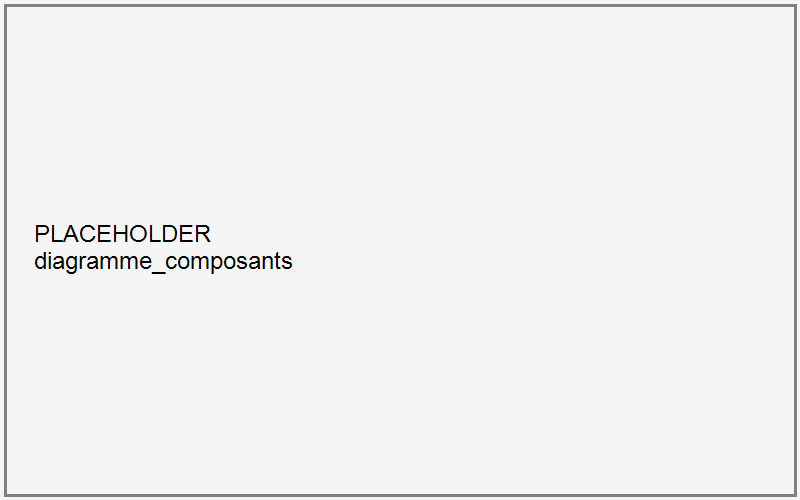
\includegraphics[width=13.5cm]{diagrammes/diagramme_composants.png}
        \caption{Diagramme de composants du backend}
        \label{fig:archi-composants}
    \end{figure}
    
    \subsubsection{Processus métier principaux}
    
    Cette section présente les diagrammes de séquence des processus transverses les plus structurants du système, communs à plusieurs sprints de réalisation. Les diagrammes de séquence propres à une fonctionnalité précise et localisée à un seul sprint seront, quant à eux, présentés directement dans le chapitre correspondant.
    
    \paragraph{Processus de déploiement d'une application.} Le processus de déploiement, illustré à la figure~\ref{fig:seq-deploiement}, se déroule selon les étapes suivantes :
    
    \begin{enumerate}
        \item Le client renseigne le formulaire de déploiement (nom, image Docker, port, ressources, bornes de mise à l'échelle) sur le portail.
        \item Le portail envoie une requête \texttt{POST /api/apps} au backend.
        \item Le backend résout l'identité effective de l'appelant (délégation MEMBER $\rightarrow$ CLIENT\_ADMIN), puis génère un nom de service unique compatible DNS.
        \item L'entité \texttt{App} est immédiatement persistée avec le statut \texttt{DEPLOYING}, un \texttt{DeploymentLog} est créé et diffusé en temps réel au portail via un flux d'événements serveur (SSE).
        \item Le backend répond immédiatement au client, \textbf{avant} que le déploiement effectif sur le cluster ne soit terminé.
        \item De manière asynchrone, le backend s'assure de l'existence de l'espace de noms du tenant et de sa \texttt{NetworkPolicy}, puis crée la ressource \texttt{Service} de Knative Serving correspondante.
        \item Knative crée une \texttt{Revision} et une \texttt{Route} ; le pod applicatif démarre (ou reste à zéro instance si le minimum de réplicas est nul).
        \item Un observateur (\textit{watcher}) Fabric8 met à jour le statut de l'application en base de données au fil de l'évolution de l'état réel du cluster, et le portail reflète ce statut en temps réel.
    \end{enumerate}
    
    
    
    \paragraph{Processus événementiel Kafka vers Knative.} Le processus déclenché par la réception d'un message Kafka, illustré à la figure~\ref{fig:seq-eventing}, se déroule selon les étapes suivantes :
    
    \begin{enumerate}
        \item Un producteur publie un message sur un sujet Kafka du cluster Strimzi.
        \item La ressource \texttt{KafkaSource}, associée à ce sujet, consomme le message et l'encapsule au format \textit{CloudEvent}, avant de le transmettre par requête HTTP au \textit{Broker} de Knative Eventing.
        \item Le \textit{Broker} évalue les filtres définis par les ressources \texttt{Trigger} enregistrées et transmet l'événement à l'application abonnée correspondante.
        \item Si l'application cible est à zéro instance, l'\textit{Activator} de Knative intercepte la requête, la met en attente, et déclenche la remise à l'échelle du service.
        \item Une fois l'instance disponible, l'application traite l'événement reçu et retourne une réponse HTTP 200.
        \item En l'absence de nouvelle sollicitation, l'application redescend automatiquement à zéro instance après une période d'inactivité.
    \end{enumerate}
    
    
    
    \section{Pilotage du projet avec SCRUM}
    \label{sec:scrum}
    
    Le cadre agile \textbf{Scrum}, retenu au chapitre précédent pour la conduite de ce projet, structure le développement en itérations courtes et fixes appelées \textit{sprints}, à l'issue desquelles un incrément de produit potentiellement livrable est produit.
    
    \subsection{Backlog du produit}
    
    Le tableau~\ref{tab:backlog} présente le backlog du produit de la plateforme. Les fonctionnalités sont organisées par module — en cohérence directe avec les besoins fonctionnels spécifiés en section~\ref{sec:besoins-fonctionnels} — et décrites sous forme de \textit{User Stories}.
    
    \refstepcounter{table}
    \label{tab:backlog}
    \begin{center}
    \textbf{\tablename~\thetable\ -- Backlog du produit}
    \end{center}
    \addcontentsline{lot}{table}{\protect\numberline{\thetable}Backlog du produit}
    
    {\small
    \renewcommand{\arraystretch}{1.3}
    \setlength{\tabcolsep}{4pt}
    \begin{longtable}{|>{\centering\arraybackslash}m{0.8cm}|>{\centering\arraybackslash}m{2.6cm}|>{\centering\arraybackslash}m{1.1cm}|>{\raggedright\arraybackslash}p{6.1cm}|>{\centering\arraybackslash}m{2.3cm}|}
    \hline
    \rowcolor{Gray}
    \textbf{ID} & \textbf{Module} & \textbf{ID US} & \textbf{User Story} & \textbf{Complexité} \\
    \hline
    \endfirsthead
    
    \hline
    \rowcolor{Gray}
    \textbf{ID} & \textbf{Module} & \textbf{ID US} & \textbf{User Story} & \textbf{Complexité} \\
    \hline
    \endhead
    
    \hline
    \multicolumn{5}{r{12.9cm}}{\textit{Suite à la page suivante}} \\
    \endfoot
    
    \endlastfoot
    
    %=========================================================
    % M1
    %=========================================================
    \multirow{5}{*}{M1} & \multirow{5}{2.6cm}{\centering Authentification \& Sécurité}
     & M1.1 & En tant qu'utilisateur, je souhaite me connecter à la plateforme via Keycloak. & Moyenne \\
    \cline{3-5}
     && M1.2 & En tant qu'utilisateur, je souhaite me déconnecter du système. & Faible \\
    \cline{3-5}
     && M1.3 & En tant qu'utilisateur, je souhaite que mon jeton d'authentification (JWT) soit automatiquement rafraîchi. & Moyenne \\
    \cline{3-5}
     && M1.4 & En tant qu'administrateur, je souhaite définir les rôles et les permissions des utilisateurs. & Élevée \\
    \cline{3-5}
     && M1.5 & En tant qu'utilisateur, je souhaite générer une clé d'API pour piloter mes déploiements depuis un pipeline CI/CD externe. & Moyenne \\
    \hline
    
    %=========================================================
    % M2
    %=========================================================
    \multirow{4}{*}{M2} & \multirow{4}{2.6cm}{\centering Utilisateurs \& équipes}
     & M2.1 & En tant qu'administrateur de compte client, je souhaite inviter un membre dans mon équipe. & Moyenne \\
    \cline{3-5}
     && M2.2 & En tant qu'administrateur de compte client, je souhaite modifier les permissions d'un membre de mon équipe. & Moyenne \\
    \cline{3-5}
     && M2.3 & En tant qu'administrateur de compte client, je souhaite retirer un membre de mon équipe. & Faible \\
    \cline{3-5}
     && M2.4 & En tant qu'administrateur de la plateforme, je souhaite gérer les comptes clients (activation, suspension, quotas). & Élevée \\
    \hline
    
    %=========================================================
    % M3
    %=========================================================
    \multirow{3}{*}{M3} & \multirow{3}{2.6cm}{\centering Infrastructure Cloud Native}
     & M3.1 & En tant que système, je souhaite créer automatiquement un espace de noms (namespace) dédié pour chaque nouveau tenant. & Élevée \\
    \cline{3-5}
     && M3.2 & En tant que système, je souhaite appliquer automatiquement une NetworkPolicy isolant chaque tenant. & Élevée \\
    \cline{3-5}
     && M3.3 & En tant qu'administrateur, je souhaite superviser l'état des nœuds du cluster Kubernetes. & Moyenne \\
    \hline
    
    %=========================================================
    % M4
    %=========================================================
    \multirow{7}{*}{M4} & \multirow{7}{2.6cm}{\centering Gestion des applications}
     & M4.1 & En tant qu'utilisateur, je souhaite déployer une application à partir d'une image Docker. & Élevée \\
    \cline{3-5}
     && M4.2 & En tant qu'utilisateur, je souhaite définir les ressources (CPU, mémoire) et les bornes de mise à l'échelle de mon application. & Moyenne \\
    \cline{3-5}
     && M4.3 & En tant qu'utilisateur, je souhaite mettre à jour la configuration d'une application déjà déployée. & Moyenne \\
    \cline{3-5}
     && M4.4 & En tant qu'utilisateur, je souhaite supprimer une application (suppression logique, conservation de l'historique de facturation). & Moyenne \\
    \cline{3-5}
     && M4.5 & En tant qu'utilisateur, je souhaite consulter l'historique des révisions d'une application. & Moyenne \\
    \cline{3-5}
     && M4.6 & En tant qu'utilisateur, je souhaite effectuer un rollback vers une révision antérieure. & Élevée \\
    \cline{3-5}
     && M4.7 & En tant qu'utilisateur, je souhaite suivre en temps réel le statut de déploiement de mon application. & Élevée \\
    \hline
    
    %=========================================================
    % M5
    %=========================================================
    \multirow{3}{*}{M5} & \multirow{3}{2.6cm}{\centering Messaging Kafka}
     & M5.1 & En tant qu'utilisateur, je souhaite créer un sujet (topic) Kafka pour mon compte. & Moyenne \\
    \cline{3-5}
     && M5.2 & En tant qu'utilisateur, je souhaite consulter la liste des sujets Kafka de mon compte. & Faible \\
    \cline{3-5}
     && M5.3 & En tant qu'utilisateur, je souhaite supprimer un sujet Kafka. & Faible \\
    \hline
    
    %=========================================================
    % M6
    %=========================================================
    \multirow{3}{*}{M6} & \multirow{3}{2.6cm}{\centering Knative Eventing}
     & M6.1 & En tant qu'utilisateur, je souhaite relier un sujet Kafka à une de mes applications déployées. & Élevée \\
    \cline{3-5}
     && M6.2 & En tant qu'utilisateur, je souhaite que mon application soit automatiquement réveillée (scale depuis zéro) à la réception d'un événement. & Élevée \\
    \cline{3-5}
     && M6.3 & En tant qu'utilisateur, je souhaite configurer un déclencheur (Trigger) avec un filtre sur le type d'événement. & Moyenne \\
    \hline
    
    %=========================================================
    % M7
    %=========================================================
    \multirow{3}{*}{M7} & \multirow{3}{2.6cm}{\centering Facturation}
     & M7.1 & En tant qu'utilisateur, je souhaite consulter la facturation de mes applications basée sur leur usage réel. & Élevée \\
    \cline{3-5}
     && M7.2 & En tant qu'administrateur, je souhaite consulter la facturation globale de tous les comptes clients. & Moyenne \\
    \cline{3-5}
     && M7.3 & En tant qu'utilisateur, je souhaite recevoir une alerte lorsque mon budget approche un seuil défini. & Moyenne \\
    \hline
    
    %=========================================================
    % M8
    %=========================================================
    \multirow{4}{*}{M8} & \multirow{4}{2.6cm}{\centering Monitoring \& Observabilité}
     & M8.1 & En tant qu'utilisateur, je souhaite consulter les journaux applicatifs de mon application en temps réel (SSE). & Élevée \\
    \cline{3-5}
     && M8.2 & En tant qu'utilisateur, je souhaite consulter les métriques (CPU, mémoire, requêtes) de mon application. & Moyenne \\
    \cline{3-5}
     && M8.3 & En tant qu'administrateur, je souhaite être alerté automatiquement en cas de redémarrage en boucle (crash loop) d'une application. & Élevée \\
    \cline{3-5}
     && M8.4 & En tant qu'administrateur, je souhaite consulter un tableau de bord Grafana de l'état global du cluster. & Moyenne \\
    \hline
    
    %=========================================================
    % M9
    %=========================================================
    \multirow{2}{*}{M9} & \multirow{2}{2.6cm}{\centering Administration plateforme}
     & M9.1 & En tant qu'administrateur, je souhaite consulter le journal d'audit des actions effectuées sur la plateforme. & Moyenne \\
    \cline{3-5}
     && M9.2 & En tant qu'administrateur, je souhaite gérer les quotas alloués à chaque compte client. & Moyenne \\
    \hline
    
    %=========================================================
    % M10
    %=========================================================
    \multirow{3}{*}{M10} & \multirow{3}{2.6cm}{\centering CI/CD}
     & M10.1 & En tant qu'équipe de développement de la plateforme, je souhaite que chaque évolution du code source déclenche automatiquement la construction d'une image Docker via Kaniko. & Élevée \\
    \cline{3-5}
     && M10.2 & En tant qu'équipe de développement de la plateforme, je souhaite que l'image construite soit automatiquement publiée sur le registre Docker Hub. & Moyenne \\
    \cline{3-5}
     && M10.3 & En tant qu'équipe de développement de la plateforme, je souhaite que la nouvelle version soit automatiquement déployée sur le cluster après publication. & Élevée \\
    \hline
    \end{longtable}
    }
    
    \subsection{Planification des Sprints}
    
    La planification cible retenue pour la conduite du projet, définissant l'ordre logique de construction des différentes briques de la plateforme, est présentée dans le tableau~\ref{tab:sprints}. Cette planification a servi de cadre méthodologique tout au long du projet ; elle reflète la démarche adoptée plutôt qu'un journal exhaustif et daté de chaque tâche réalisée, celui-ci n'ayant pas fait l'objet d'une documentation formelle systématique sprint par sprint.
    
    \begin{table}[H]
    \begin{center}
    \begin{tabular}{|c{2cm}|l{11cm}|}
    \hline
    \textbf{Sprint} & \textbf{Objectif principal} \\
    \hline
    Sprint 0  & Infrastructure Kubernetes \\
    \hline
    Sprint 1  & Knative Serving \\
    \hline
    Sprint 2  & Kafka \& Strimzi \\
    \hline
    Sprint 3  & Knative Eventing \\
    \hline
    Sprint 4  & Authentification \& Sécurité \\
    \hline
    Sprint 5  & Gestion des applications + début du pipeline CI/CD Backend \\
    \hline
    Sprint 6  & Gestion Kafka et Eventing côté Backend \\
    \hline
    Sprint 7  & Monitoring, Logs et Observabilité \\
    \hline
    Sprint 8  & Frontend + pipeline CI/CD Frontend \\
    \hline
    Sprint 9  & Finalisation du Frontend \\
    \hline
    Sprint 10 & Optimisation CI/CD et déploiement \\
    \hline
    Sprint 11 & Tests, validation et corrections \\
    \hline
    Sprint 12 & Documentation et préparation de la soutenance \\
    \hline
    \end{tabular}
    \caption{Planification des sprints du projet}
    \label{tab:sprints}
    \end{center}
    \end{table}
    
    Le détail de la réalisation de chacun de ces sprints (analyse, conception et implémentation) est présenté progressivement dans les chapitres suivants, regroupés par \textit{release}.
    
    
    \section{Environnement de travail}
    
    \subsection{Environnement matériel de développement}
    \label{sec:env-materiel}

    \subsubsection{Poste de développement}

    Le développement de la plateforme (backend, portails web, manifestes Kubernetes) a été réalisé sur un poste de travail disposant des caractéristiques suivantes :

    \begin{itemize}
        \item \textbf{Modèle} : Ordinateur portable MSI GF63 Thin 10SC
        \item \textbf{Système d'exploitation} : Windows 11 Pro (64 bits)
        \item \textbf{Processeur} : Intel(R) Core(TM) i7-10750H CPU @ 2.60GHz
        \item \textbf{Mémoire RAM} : 16 Go
        \item \textbf{Stockage} : 2 $\times$ SSD 512 Go (TEAM T253 512GB + Micron 2210 512GB), soit environ 1 To au total
    \end{itemize}

    \subsubsection{Cluster de déploiement (infrastructure Kubernetes)}

    Le déploiement et l'exploitation de la plateforme se sont appuyés sur un cluster Kubernetes composé de trois machines virtuelles sous Ubuntu 24, administrées via un utilisateur \texttt{sysadmin} : un nœud de plan de contrôle (\textit{control-plane}) et deux nœuds de travail (\textit{workers}), sur lesquels sont exécutés l'ensemble des composants de la plateforme ainsi que les applications des clients.

    \begin{table}[H]
    \begin{center}
    \begin{tabular}{|l{3cm}|l{4cm}|l{3cm}|l{3cm}|}
    \hline
    \textbf{Nom de la VM} & \textbf{Ressources} & \textbf{Système} & \textbf{Rôle} \\
    \hline
    Master   & 4 vCPU, 8 Go RAM, 50 Go disque & Ubuntu 24 & Plan de contrôle (control-plane) \\
    \hline
    Worker 1 & 4 vCPU, 8 Go RAM, 50 Go disque & Ubuntu 24 & Nœud de travail \\
    \hline
    Worker 2 & 4 vCPU, 8 Go RAM, 50 Go disque & Ubuntu 24 & Nœud de travail \\
    \hline
    \end{tabular}
    \caption{Caractéristiques des machines virtuelles du cluster Kubernetes}
    \label{tab:vms-cluster}
    \end{center}
    \end{table}

    Le cluster utilise Cilium comme interface réseau de conteneurs (CNI), MetalLB pour l'attribution d'adresses IP aux services de type \textit{LoadBalancer} dans un environnement dépourvu de répartiteur de charge natif, et Kourier comme passerelle d'entrée (\textit{ingress gateway}) pour Knative Serving.
    
    \subsection{Environnement logiciel de développement}
    
    \subsubsection{Langages de programmation}

    Le tableau~\ref{tab:langages} présente les langages de programmation utilisés pour la réalisation de la plateforme.

    \begin{table}[H]
    \begin{center}
    \begin{tabular}{|l{3.2cm}|p{10cm}|}
    \hline
    \textbf{Langage} & \textbf{Description} \\
    \hline
    Java & Langage principal du backend applicatif (\texttt{backend-api}), développé avec Spring Boot. \\
    \hline
    TypeScript / JavaScript & Langages utilisés pour le développement des deux portails web React (\texttt{web-portal} et \texttt{admin-console}). \\
    \hline
    YAML & Langage de description déclarative utilisé pour l'ensemble des manifestes Kubernetes, Knative, Strimzi, ainsi que pour la configuration de l'application (\texttt{application.yml}). \\
    \hline
    Shell (Bash) & Utilisé pour les scripts de déploiement, d'initialisation du cluster et d'automatisation des tâches d'exploitation. \\
    \hline
    Groovy & Langage utilisé pour l'écriture des \textit{Jenkinsfiles} du pipeline CI/CD. \\
    \hline
    \end{tabular}
    \caption{Langages de programmation utilisés}
    \label{tab:langages}
    \end{center}
    \end{table}
    
    \subsubsection{Frameworks et bibliothèques}

    Le tableau~\ref{tab:frameworks} présente les principaux frameworks et bibliothèques utilisés pour le développement de la plateforme.

    \begin{table}[H]
    \begin{center}
    \begin{tabular}{|l{3.2cm}|p{10cm}|}
    \hline
    \textbf{Nom} & \textbf{Description} \\
    \hline
    Spring Boot & Framework backend utilisé pour l'exposition de l'API REST, l'injection de dépendances, la sécurité (Spring Security) et l'accès aux données (Spring Data JPA). \\
    \hline
    Fabric8 Kubernetes Client & Bibliothèque Java utilisée par le backend pour orchestrer les ressources Kubernetes natives et les ressources personnalisées (CRD) de Knative et Strimzi. \\
    \hline
    React & Bibliothèque utilisée pour le développement des interfaces graphiques du portail client et de la console d'administration. \\
    \hline
    PostgreSQL / JPA-Hibernate & Système de gestion de base de données relationnelle et couche de mapping objet-relationnel utilisés pour la persistance des entités métier. \\
    \hline
    Keycloak (OpenID Connect) & Bibliothèque d'intégration utilisée côté backend et frontend pour l'authentification et la validation des jetons JWT. \\
    \hline
    \end{tabular}
    \caption{Frameworks et bibliothèques utilisés}
    \label{tab:frameworks}
    \end{center}
    \end{table}

    \subsubsection{Outils DevOps et déploiement}

    Le tableau~\ref{tab:outils-devops} présente les outils utilisés pour le développement, les tests, la conteneurisation, l'intégration continue et la modélisation UML de la plateforme.

    \begin{table}[H]
    \begin{center}
    \begin{tabular}{|l{3.2cm}|p{10cm}|}
    \hline
    \textbf{Nom} & \textbf{Description} \\
    \hline
    Visual Studio Code & Environnement de développement intégré léger et extensible, utilisé pour le développement du backend Spring Boot, des deux applications frontend React, ainsi que pour la rédaction des manifestes Kubernetes et des scripts de déploiement. \\
    \hline
    GitHub & Plateforme d'hébergement du code source et de gestion de versions, utilisée pour le suivi des évolutions du projet et le déclenchement des pipelines d'intégration continue. \\
    \hline
    Postman & Outil de test et de documentation des API REST, utilisé pour valider manuellement le comportement des différents points d'accès exposés par le backend avant leur intégration dans les interfaces graphiques. \\
    \hline
    Docker & Utilisé pour la construction et l'exécution locale des images de conteneurs avant leur publication sur le registre Docker Hub par la chaîne CI/CD. \\
    \hline
    Jenkins et Kaniko & Utilisés pour l'automatisation de la construction, de la publication et du déploiement continu des composants de la plateforme, Kaniko permettant de construire les images sans démon Docker privilégié à l'intérieur du cluster. \\
    \hline
    kubectl & Interface en ligne de commande de Kubernetes, utilisée quotidiennement pour l'inspection de l'état du cluster, le déploiement manuel de ressources lors des phases de mise au point, et le diagnostic des incidents. \\
    \hline
    PlantUML & Outil de modélisation UML en tant que code, utilisé pour la production des diagrammes de cas d'utilisation, de classes, de composants, de déploiement et de séquence présentés dans ce mémoire, à partir de scripts textuels versionnés avec le code source. \\
    \hline
    \end{tabular}
    \caption{Outils DevOps et déploiement utilisés}
    \label{tab:outils-devops}
    \end{center}
    \end{table}
    
    
    \section{Conclusion}
    
    Ce chapitre a permis de formaliser les besoins fonctionnels et non fonctionnels de la plateforme, de préciser les acteurs qui interagissent avec le système et le diagramme de cas d'utilisation général qui en découle, puis de présenter l'analyse globale de la plateforme (diagramme de classes, architecture logique et physique, processus métier principaux) et le pilotage du projet au travers du Product Backlog et de la planification des sprints selon la méthode Scrum. L'environnement de travail matériel et logiciel utilisé pour la réalisation du projet a également été détaillé. Le détail de chaque sprint (description textuelle des cas d'utilisation, diagrammes de séquence spécifiques, réalisation) est développé progressivement dans les chapitres suivants, regroupés par release.
    
\chapter*{chapitre 3}
\markboth{Chapitre 3 }{3 Release 0 : Mise en place de la plateforme Cloud Native} %pour afficher l'entete
 \addcontentsline{toc}{chapter}{3 Release 0 : Mise en place de la plateforme Cloud Native}

\textbf{\Huge Release 0 : Mise en place de la plateforme Cloud Native}

\setcounter{chapter}{3}
\setcounter{section}{0}

\section{Introduction de la Release}

La Release 0 constitue le socle technique de l'ensemble du projet. Elle regroupe les trois premiers sprints (Sprint 0, Sprint 1 et Sprint 2), dont l'objectif commun est de mettre en place les briques d'infrastructure \textit{cloud native} sur lesquelles reposeront, dans les releases suivantes, la logique métier applicative et les interfaces utilisateur. Aucune de ces briques n'expose directement de fonctionnalité à un utilisateur final : il s'agit d'un travail de fondation, validant que le cluster Kubernetes, la capacité de mise à l'échelle serverless (Knative Serving) et le bus d'événements (Kafka/Strimzi) sont opérationnels avant que le backend applicatif ne vienne s'y raccorder à partir de la Release 1. Conformément à cette nature purement technique, les sprints de cette release ne comportent pas de diagramme de cas d'utilisation : ceux-ci n'apparaîtront qu'à partir du moment où une fonctionnalité devient accessible à un acteur humain (Release 1 et suivantes).

Chaque section qui suit adopte la même démarche : partir du problème concret que la brique doit résoudre, justifier le choix technologique retenu (et non un autre), puis montrer comment ce choix s'intègre réellement dans la configuration du cluster telle qu'elle existe dans ce dépôt. Le Sprint 0 construit le socle Kubernetes et le réseau qui le rend exploitable depuis l'extérieur ; le Sprint 1 y ajoute la capacité d'exécution serverless ; le Sprint 2 y ajoute la communication événementielle. Les trois sprints s'enchaînent donc de façon strictement incrémentale, chacun s'appuyant sur ce que le précédent a mis en place. L'exploitation programmatique de cette infrastructure par le backend applicatif — au travers des classes \texttt{KnativeService}, \texttt{KafkaService} et \texttt{EventingService} — est présentée dans les chapitres consacrés au développement du backend ; ce chapitre se limite à ce qui a été installé, configuré et validé au niveau du cluster lui-même.

\section{Sprint 0 : Socle Kubernetes et réseau}

\subsection{Introduction}

Ce premier sprint a pour objectif d'établir le cluster Kubernetes qui hébergera l'ensemble des composants de la plateforme, ainsi que l'ensemble des briques réseau nécessaires pour le rendre isolable par tenant et accessible depuis l'extérieur.

\subsection{Objectifs du Sprint}

\begin{itemize}
    \item Mettre en place un cluster Kubernetes multi-nœuds.
    \item Configurer une interface réseau de conteneurs (CNI) permettant l'application de règles d'isolation réseau entre espaces de noms.
    \item Mettre en place un mécanisme d'attribution d'adresses IP externes pour les services de type \textit{LoadBalancer}, le cluster n'étant pas hébergé chez un fournisseur cloud proposant nativement ce service.
    \item Mettre en place une passerelle d'entrée HTTP compatible avec la future couche serverless (Knative Serving, Sprint 1).
    \item Définir la convention d'organisation des espaces de noms (un espace de noms dédié à la plateforme, un espace de noms par tenant).
\end{itemize}

\subsection{Sprint Backlog}

\begin{table}[!ht]
\begin{center}
     \begin{tabular}{|l{6cm}|l{5.5cm}|l{2.5cm}|}
     \hline
     \textbf{User Story} & \textbf{Critère d'acceptation} & \textbf{Statut} \\
     \hline
     En tant qu'exploitant, je veux disposer d'un cluster Kubernetes fonctionnel & \texttt{kubectl get nodes} retourne les trois nœuds du cluster (un \textit{control-plane}, deux \textit{workers}) à l'état \texttt{Ready} & Réalisé \\
     \hline
     En tant qu'exploitant, je veux isoler le trafic réseau entre tenants & Une ressource \texttt{NetworkPolicy} de type \textit{default-deny} peut être appliquée dans un espace de noms et bloque effectivement le trafic non autorisé & Réalisé \\
     \hline
     En tant qu'exploitant, je veux pouvoir exposer un service avec une IP externe & Un service Kubernetes de type \texttt{LoadBalancer} se voit attribuer une adresse IP externe joignable, sans dépendre d'un fournisseur cloud managé & Réalisé \\
     \hline
     En tant qu'exploitant, je veux disposer d'une passerelle d'entrée HTTP prête pour Knative & Le \textit{Service} Kubernetes exposé par Kourier reçoit une IP externe via MetalLB et route le trafic vers le \textit{namespace} \texttt{kourier-system} & Réalisé \\
     \hline
     \end{tabular}
     \caption{Sprint Backlog — Sprint 0}
     \label{tab:sb-sprint0}
     \end{center}
\end{table}

\subsection{Kubernetes}

Le besoin de départ de ce sprint est simple à énoncer mais structurant pour tout le reste du projet : la plateforme doit pouvoir exécuter, isoler et exposer un nombre a priori non borné d'applications appartenant à des clients (tenants) différents, sans que ceux-ci ne puissent s'atteindre entre eux ni accéder aux composants internes de la plateforme (base de données, Keycloak). \textbf{Kubernetes}~\citep{KubernetesDoc} a été retenu comme socle d'orchestration parce qu'il fournit nativement les deux primitives dont dépend directement ce besoin : l'espace de noms (\textit{namespace}), qui sert d'unité d'isolation logique par tenant, et la ressource \texttt{NetworkPolicy}, qui permet de restreindre le trafic réseau entre pods au niveau de ces espaces de noms. Kubernetes fournit également, au-delà de ces deux primitives, les briques de base sur lesquelles s'appuient directement les sprints suivants : le \textit{pod} comme unité d'exécution d'un conteneur, le \textit{Service} comme point d'accès stable à un ensemble de pods, et surtout un modèle extensible par ressources personnalisées (\textit{Custom Resource Definitions}), sans lequel ni Knative (Sprint 1) ni Strimzi (Sprint 2) — tous deux des opérateurs Kubernetes qui ajoutent leurs propres types de ressources — ne pourraient fonctionner.

\subsection{Architecture du cluster}

Le cluster est composé de trois machines virtuelles sous Ubuntu 24 : un nœud de plan de contrôle (\textit{control-plane}) et deux nœuds de travail (\textit{workers}). Leurs caractéristiques exactes sont détaillées au tableau~\ref{tab:vms-cluster} du chapitre précédent (environnement matériel). Le choix d'un cluster à trois nœuds plutôt qu'un cluster mono-nœud (par exemple k3s en mode \textit{single-node}) répond au besoin de répartir la charge des applications tenants sur plusieurs machines, tout en gardant un nombre de nœuds réaliste pour un projet de fin d'études mené par une seule personne. Le cluster est auto-hébergé sur ces VM plutôt que confié à un service Kubernetes managé (EKS, GKE, AKS) : ce choix n'est pas documenté comme un arbitrage de coût ou de performance dans le dépôt du projet, il est simplement constaté comme la configuration retenue et exploitée tout au long du développement.

Le chemin logique suivi par ce sprint part de ce cluster nu et l'enrichit progressivement : cluster Kubernetes~$\rightarrow$~CNI (Cilium)~$\rightarrow$~isolation par \textit{namespace}~$\rightarrow$~exposition externe (MetalLB puis Kourier)~$\rightarrow$~socle prêt pour Knative Serving. Les sous-sections suivantes détaillent chacune de ces briques.

\subsection{Cilium}

Kubernetes ne fournit pas nativement de mise en réseau des conteneurs : cette fonction est déléguée à une interface réseau de conteneurs (\textit{Container Network Interface}, CNI), un plugin chargé d'attribuer une adresse IP à chaque pod et d'acheminer le trafic entre eux. Toutes les CNI ne se valent cependant pas sur un point précis et déterminant pour ce projet : le support des ressources \texttt{NetworkPolicy}. Des CNI minimalistes comme Flannel, par exemple, ne l'implémentent pas du tout ; d'autres, comme Calico, l'implémentent mais avec un mécanisme de filtrage \textit{iptables} plus classique. \textbf{Cilium}~\citep{CiliumDoc} a été retenu ici précisément parce qu'il supporte nativement les \texttt{NetworkPolicy} et s'appuie sur eBPF pour appliquer ce filtrage directement au niveau du noyau Linux, avec un coût de performance réduit par rapport à un filtrage \textit{iptables} traditionnel. Ce choix n'a pas fait l'objet d'une évaluation comparative formalisée dans le projet (pas de benchmark Cilium/Calico/Flannel réalisé) : il s'agit d'un choix technique assumé en amont, dont la conséquence directe est de rendre possible l'isolation multi-tenant détaillée à la sous-section suivante.

\subsection{NetworkPolicy}

Une ressource \texttt{NetworkPolicy} définit, pour un ensemble de pods sélectionnés dans un \textit{namespace}, quel trafic entrant (\textit{ingress}) et sortant (\textit{egress}) est autorisé ; tout ce qui n'est pas explicitement autorisé par une règle est refusé dès qu'au moins une \texttt{NetworkPolicy} s'applique au pod. C'est ce mécanisme, rendu utilisable par Cilium, qui porte l'isolation réseau entre tenants de la plateforme : chaque \textit{namespace} tenant reçoit une politique de type \textit{default-deny} qui n'autorise que le trafic strictement nécessaire au fonctionnement de l'application (accès depuis la passerelle d'entrée, résolution DNS, accès au bus Kafka partagé), et bloque explicitement tout accès direct vers un autre \textit{namespace} tenant ou vers les composants internes de la plateforme (\texttt{platform} : base de données, Keycloak).

Le manifeste ci-dessous, extrait de \texttt{k8s/tenant/network-policy.yaml} (fichier réellement versionné dans le dépôt), montre la structure de cette politique :

\begin{lstlisting}[language=, caption={Extrait de \texttt{k8s/tenant/network-policy.yaml} — politique \textit{default-deny} appliquée à chaque namespace tenant}, label={lst:networkpolicy-yaml}]
apiVersion: networking.k8s.io/v1
kind: NetworkPolicy
metadata:
  name: tenant-default-isolation
  namespace: NAMESPACE_PLACEHOLDER
spec:
  podSelector: {}
  policyTypes:
    - Ingress
    - Egress
  ingress:
    - from:
        - podSelector: {}
    - from:
        - namespaceSelector:
            matchLabels:
              kubernetes.io/metadata.name: kourier-system
    - from:
        - namespaceSelector:
            matchLabels:
              kubernetes.io/metadata.name: knative-serving
    - from:
        - namespaceSelector:
            matchLabels:
              kubernetes.io/metadata.name: monitoring
  egress:
    - to:
        - podSelector: {}
    - to:
        - namespaceSelector:
            matchLabels:
              kubernetes.io/metadata.name: kube-system
      ports:
        - protocol: UDP
          port: 53
        - protocol: TCP
          port: 53
    - to:
        - namespaceSelector:
            matchLabels:
              kubernetes.io/metadata.name: kafka
    - to:
        - namespaceSelector:
            matchLabels:
              kubernetes.io/metadata.name: knative-serving
    - to:
        - namespaceSelector:
            matchLabels:
              kubernetes.io/metadata.name: kourier-system
\end{lstlisting}

Le tableau~\ref{tab:networkpolicy-rules} résume ces règles.

\begin{table}[!ht]
\begin{center}
     \begin{tabular}{|l{3cm}|l{9cm}|}
     \hline
     \textbf{Sens} & \textbf{Règle autorisée} \\
     \hline
     Ingress & Trafic intra-namespace (\texttt{podSelector} vide) ; trafic depuis \texttt{kourier-system}, \texttt{knative-serving} et \texttt{monitoring} \\
     \hline
     Egress & Trafic intra-namespace ; DNS (\texttt{kube-system}, UDP/TCP 53) ; \texttt{kafka} ; \texttt{knative-serving} ; \texttt{kourier-system} \\
     \hline
     \end{tabular}
     \caption{Règles de la \texttt{NetworkPolicy} \textit{default-deny} appliquée à chaque namespace tenant}
     \label{tab:networkpolicy-rules}
     \end{center}
\end{table}

Ce fichier \texttt{NAMESPACE\_PLACEHOLDER} était destiné à être appliqué manuellement (\texttt{kubectl apply}, un \textit{namespace} à la fois) sur les \textit{namespaces} tenants déjà présents sur le cluster au moment du ticket d'audit ayant motivé cette politique. Cette application manuelle \textbf{n'a en réalité jamais été effectuée} : le manifeste existe dans le dépôt à titre de modèle documenté, mais rien ne prouve qu'il a été exécuté sur le cluster réel pour les \textit{namespaces} concernés.

Ce constat n'invalide toutefois pas complètement la protection de ces \textit{namespaces} préexistants : le backend applicatif recrée automatiquement cette même politique, par un mécanisme indépendant du fichier YAML, à chaque déploiement d'application dans un \textit{namespace} tenant — y compris un \textit{namespace} déjà existant (mécanisme détaillé dans les chapitres consacrés au développement du backend). Ce dépôt ne permet toutefois pas de savoir, pour chacun des \textit{namespaces} tenants existants, si un déploiement a eu lieu depuis la mise en service de cette automatisation : seule une vérification directe sur le cluster (\texttt{kubectl get networkpolicy -n <namespace>}) peut le confirmer ou l'infirmer.

\subsection{MetalLB}

Un service Kubernetes de type \texttt{LoadBalancer} délègue normalement l'attribution d'une adresse IP externe au fournisseur cloud sous-jacent (AWS, GCP, Azure...). Sur un cluster auto-hébergé sur des VM, comme c'est le cas ici, il n'existe aucun contrôleur pour répondre à cette demande : un tel service reste indéfiniment à l'état \texttt{Pending}, sans adresse IP externe attribuée. \textbf{MetalLB}~\citep{MetalLBDoc} a été retenu pour combler ce manque : il implémente lui-même ce contrôleur, en gérant une réserve d'adresses IP du réseau local (mode \textit{Layer2}, le plus simple à opérer, par diffusion ARP) qu'il attribue aux services \texttt{LoadBalancer} au fur et à mesure de leur création. C'est ce mécanisme qui permet, par exemple, au service \texttt{platform-api} du backend (cf. \texttt{k8s/backend/deployment.yaml}) d'être exposé sur une IP externe joignable depuis l'extérieur du cluster. Les ressources précises de configuration de MetalLB (\texttt{IPAddressPool}, \texttt{L2Advertisement}) et la plage d'adresses effectivement réservée n'ont pas été versionnées dans le dépôt du projet ; elles ne sont donc pas reproduites ici pour éviter d'avancer des valeurs non vérifiables.

\subsection{Kourier}

MetalLB résout le problème de l'attribution d'une IP externe à un \textit{Service} Kubernetes, mais ne dit rien du routage applicatif du trafic HTTP une fois cette IP atteinte. Ce rôle revient à une passerelle d'entrée (\textit{ingress gateway}). Knative Serving (Sprint 1) ne fonctionne pas sans une telle passerelle : c'est elle qui reçoit le trafic HTTP externe et le route vers le bon service Knative, dans le bon \textit{namespace} tenant, en fonction du nom d'hôte de la requête. \textbf{Kourier}~\citep{KourierDoc} a été choisie pour ce rôle plutôt qu'une solution basée sur Istio, pour sa légèreté : Kourier ne fait que le routage HTTP nécessaire à Knative, sans ajouter la complexité d'un maillage de services complet (\textit{mTLS} entre services, politiques de trafic avancées) dont la plateforme n'a pas l'usage. Kourier s'installe comme un \textit{Service} Kubernetes de type \texttt{LoadBalancer} dans le \textit{namespace} \texttt{kourier-system} : c'est donc MetalLB qui lui attribue son IP externe, complétant ainsi la chaîne d'exposition mise en place par ce sprint : MetalLB (IP externe) $\rightarrow$ Kourier (routage HTTP) $\rightarrow$ Knative Serving (Sprint 1).

\subsection{Réalisation}

La convention d'espaces de noms retenue distingue l'espace de noms \texttt{platform} (composants de la plateforme elle-même : backend, portails, base de données, Keycloak) des espaces de noms créés dynamiquement, un par tenant, lors du premier déploiement d'une application par ce client. Cette création dynamique de l'espace de noms tenant, ainsi que de sa \texttt{NetworkPolicy} associée présentée ci-dessus, est prise en charge automatiquement par le backend applicatif ; le mécanisme précis de cette automatisation relève du développement du backend et est détaillé dans les chapitres qui y sont consacrés.

\subsection{Difficultés rencontrées et solutions apportées}
\label{sec:sprint0-difficultes}

La configuration du cluster (nœuds, CNI Cilium, MetalLB, passerelle Kourier) a été réalisée directement sur l'infrastructure, à l'aide des outils en ligne de commande usuels (\texttt{kubeadm}, \texttt{helm}, \texttt{kubectl}), sans être formalisée sous forme de manifestes versionnés dans le dépôt du projet. Seule la \texttt{NetworkPolicy} tenant (fichier \texttt{k8s/tenant/network-policy.yaml}) et les ressources applicatives (\texttt{k8s/backend}, \texttt{k8s/frontend}, \texttt{k8s/admin}, \texttt{k8s/monitoring}, \texttt{k8s/backup}) sont versionnées. Cette absence d'infrastructure-as-code pour le socle du cluster (nœuds, CNI, MetalLB, Kourier, ainsi que le cluster Kafka provisionné au Sprint 2) constitue une limite identifiée du projet : elle signifie qu'une reconstruction du cluster à l'identique ne peut aujourd'hui reposer que sur la mémoire opérationnelle des commandes exécutées, plutôt que sur un ensemble de manifestes ou de scripts rejouables. Cette limite est reprise au chapitre de validation, et ne sera pas répétée dans le détail aux sprints suivants, où elle s'applique de la même manière (Sprint 2, section~\ref{sec:sprint2-difficultes}).

\subsection{Validation}

La disponibilité et la bonne configuration du socle mis en place par ce sprint peuvent être vérifiées à l'aide des commandes suivantes, exécutées directement sur le cluster :

\begin{lstlisting}[language=bash, caption={Commandes de validation du socle Kubernetes (Sprint 0)}, label={lst:validation-sprint0}]
# Etat des noeuds du cluster
kubectl get nodes -o wide

# Namespaces existants (platform + un namespace par tenant)
kubectl get namespaces

# NetworkPolicy appliquees, tous namespaces confondus
kubectl get networkpolicy -A

# Etat de Cilium (CNI) sur le cluster
cilium status

# Adresse(s) IP geree(s) par MetalLB
kubectl get ipaddresspool -n metallb-system

# Service Kourier et son IP externe attribuee par MetalLB
kubectl get svc -n kourier-system
\end{lstlisting}

% TODO (Adel) : inserer ici les captures d'ecran reelles de l'execution
% de ces commandes (sortie de kubectl get nodes -o wide, kubectl get
% networkpolicy -A, cilium status, kubectl get ipaddresspool -n
% metallb-system, kubectl get svc -n kourier-system), afin de prouver
% concretement l'etat du cluster au moment de la redaction. Aucune de
% ces captures n'est disponible dans memoire/captures actuellement.

\subsection{Résultat obtenu}

Au terme de ce sprint, un cluster Kubernetes opérationnel à trois nœuds est disponible, avec isolation réseau possible entre espaces de noms (Cilium), capacité d'exposition de services externes (MetalLB) et passerelle de routage HTTP prête à recevoir Knative Serving (Kourier).

\subsection{Conclusion du Sprint}

Ce sprint a posé les fondations d'infrastructure indispensables à la suite du projet. Le sprint suivant s'appuie directement sur ce cluster pour y déployer Knative Serving.


\section{Sprint 1 : Knative Serving}

\subsection{Introduction}

Ce sprint a pour objectif d'intégrer Knative Serving au cluster mis en place au Sprint 0, afin de disposer de la capacité à exécuter des applications conteneurisées avec mise à l'échelle automatique, y compris jusqu'à zéro instance.

\subsection{Objectifs du Sprint}

\begin{itemize}
    \item Installer et configurer Knative Serving sur le cluster, en s'appuyant sur la passerelle Kourier mise en place au Sprint 0.
    \item Valider la capacité à créer, par programmation, une ressource \texttt{Service} Knative à partir d'une image Docker.
    \item Mettre en place la création automatique de l'espace de noms d'un tenant et de sa \texttt{NetworkPolicy} lors du premier déploiement.
    \item Valider le comportement d'autoscaling et de mise à zéro instance (\textit{scale-to-zero}).
\end{itemize}

\subsection{Sprint Backlog}

\begin{table}[!ht]
\begin{center}
     \begin{tabular}{|l{6cm}|l{5.5cm}|l{2.5cm}|}
     \hline
     \textbf{User Story} & \textbf{Critère d'acceptation} & \textbf{Statut} \\
     \hline
     En tant qu'exploitant, je veux que Knative Serving soit opérationnel sur le cluster & Le déploiement d'une ressource \texttt{Service} de test (\texttt{serving.knative.dev/v1}) atteint la condition \texttt{Ready=True} et expose une URL & Réalisé \\
     \hline
     En tant que développeur backend, je veux pouvoir créer une ressource Knative Service par programmation & La méthode \texttt{KnativeService.deploy(...)} crée effectivement la ressource via le client Fabric8, sans intervention manuelle & Réalisé \\
     \hline
     En tant qu'exploitant, je veux que l'espace de noms d'un tenant soit créé automatiquement au premier déploiement & \texttt{ensureNamespaceExists} crée le \textit{namespace} et sa \texttt{NetworkPolicy} s'ils n'existent pas encore, et ne fait rien s'ils existent déjà (idempotence) & Réalisé \\
     \hline
     \end{tabular}
     \caption{Sprint Backlog — Sprint 1}
     \label{tab:sb-sprint1}
     \end{center}
\end{table}

\subsection{Pourquoi Knative ?}

Le besoin adressé par ce sprint découle directement du positionnement \textit{serverless} de la plateforme, exprimé dans les besoins non fonctionnels du chapitre précédent (élasticité et efficience des ressources) : une application cliente déployée sur la plateforme ne doit consommer aucune ressource de calcul lorsqu'elle est inactive, et doit pouvoir remonter en charge automatiquement dès qu'elle reçoit du trafic. Un simple \texttt{Deployment} Kubernetes ne répond que partiellement à ce besoin : il permet bien de faire varier le nombre de \textit{pods} (via un \texttt{HorizontalPodAutoscaler}), mais il ne descend jamais à zéro instance de lui-même, et ne gère ni le routage progressif du trafic entre versions, ni le réveil à la demande d'une application totalement arrêtée. \textbf{Knative Serving}~\citep{KnativeServingDoc} a été retenu précisément parce qu'il ajoute cette couche par-dessus Kubernetes, sous la forme d'une ressource personnalisée \texttt{Service} (\texttt{serving.knative.dev/v1}) qui gère elle-même la création des \textit{Revisions}, le routage du trafic entre elles, et surtout la mise à l'échelle jusqu'à zéro pod en l'absence de trafic.

\subsection{Fonctionnement de Knative Serving}

Une ressource Knative \texttt{Service} n'est jamais exécutée directement : chaque modification de sa spécification (nouvelle image, nouvelle configuration) donne naissance à une \textit{Revision}, un instantané immuable de cette configuration. C'est la \textit{Revision} active qui est effectivement déployée sous forme de \textit{pods}, eux-mêmes gérés par le composant d'autoscaling de Knative (\textit{Knative Pod Autoscaler}) en fonction du trafic réellement reçu. La chaîne est donc : \texttt{Service} Knative $\rightarrow$ \textit{Revision} $\rightarrow$ \textit{pod(s)}, avec un nombre de \textit{pods} qui varie automatiquement entre les bornes \texttt{minScale} et \texttt{maxScale} définies sur la \textit{Revision}, jusqu'à zéro si \texttt{minScale=0} et qu'aucun trafic n'est reçu.

\subsection{Architecture}

La figure~\ref{fig:sprint1-flux} illustre le chemin suivi par une requête HTTP externe jusqu'à un service Knative, tel qu'il résulte de la combinaison des briques mises en place aux Sprints 0 et 1.

\begin{figure}[H]
\centering
\begin{tikzpicture}[node distance=1.6cm, every node/.style={font=\small}]
\tikzstyle{box}=[draw, rounded corners, minimum width=3.2cm, minimum height=0.9cm, align=center, fill=Gray!20]
\node[box] (client) {Client externe};
\node[box, right=2.2cm of client] (metallb) {MetalLB\\(IP LoadBalancer)};
\node[box, right=2.2cm of metallb] (kourier) {Kourier\\(ingress gateway)};
\node[box, right=2.2cm of kourier] (ksvc) {Knative Service\\(namespace tenant)};
\draw[->, thick] (client) -- (metallb);
\draw[->, thick] (metallb) -- (kourier);
\draw[->, thick] (kourier) -- (ksvc);
\end{tikzpicture}
\caption{Chemin d'une requête HTTP externe vers une application tenant (MetalLB $\rightarrow$ Kourier $\rightarrow$ Knative Service)}
\label{fig:sprint1-flux}
\end{figure}

\subsection{Intégration avec Kubernetes}

Une ressource \texttt{Service} Knative reste, en dernière analyse, une ressource personnalisée Kubernetes (\textit{Custom Resource}) au même titre que celles introduites par Strimzi au Sprint 2 : elle est stockée dans etcd comme n'importe quelle autre ressource, et suit le même modèle de \textit{namespace} que les objets Kubernetes natifs. C'est ce qui permet de rattacher directement chaque service Knative au \textit{namespace} tenant créé au Sprint 0, et de le faire bénéficier automatiquement de la \texttt{NetworkPolicy} \textit{default-deny} qui y est appliquée. Avant même de créer la ressource \texttt{Service} Knative elle-même, le backend doit donc garantir que ce \textit{namespace} et cette politique existent : c'est le rôle des méthodes \texttt{ensureNamespaceExists} et \texttt{ensureNetworkPolicyExists}, appelées systématiquement en tête de \texttt{deploy(...)}.

\subsection{Intégration Fabric8}

Ce sprint introduit la classe \texttt{KnativeService} du backend (\texttt{backend-api/src/main/java/com/platform/api/app/KnativeService.java}), qui encapsule l'ensemble des interactions avec Knative Serving au travers du client \textbf{Fabric8}~\citep{Fabric8Doc}. La création d'un service Knative est réalisée via l'API générique des ressources personnalisées de Fabric8 (\texttt{genericKubernetesResources}), Knative Serving ne disposant pas, au moment de la réalisation du projet, d'un client Java typé officiel comparable à celui existant pour les ressources natives de Kubernetes (\texttt{Namespace}, \texttt{NetworkPolicy}), pour lesquelles Fabric8 fournit des classes générées et un \textit{builder} typé. Ce contraste est visible directement dans le code : \texttt{NetworkPolicyBuilder} (typé, avec autocomplétion et vérification à la compilation) d'un côté, \texttt{GenericKubernetesResourceBuilder} (générique, avec accès aux champs via des \texttt{Map<String,Object>}) de l'autre. Ce choix a été assumé pour l'ensemble des ressources personnalisées manipulées côté Kubernetes, y compris Knative Eventing (Sprint 3) — mais pas pour Kafka, comme précisé au Sprint 2.

\subsection{Déploiement d'une application}

La méthode \texttt{deploy(...)} construit le manifeste Knative Service (méthode privée \texttt{buildKnativeManifest}) à partir de l'image Docker, du port, des ressources CPU/mémoire et des bornes \texttt{minScale}/\texttt{maxScale} demandées, puis le soumet au cluster. L'extrait ci-dessous, tiré du code réel du backend, illustre cette construction :

\begin{lstlisting}[language=Java, caption={Extrait de \texttt{KnativeService.buildKnativeManifest} — construction du manifeste Knative Service via l'API générique Fabric8}, label={lst:knative-manifest}]
return new GenericKubernetesResourceBuilder()
    .withApiVersion("serving.knative.dev/v1")
    .withKind("Service")
    .withNewMetadata()
        .withName(name)
        .withNamespace(namespace)
    .endMetadata()
    .addToAdditionalProperties("spec", Map.of(
        "template", Map.of(
            "metadata", Map.of(
                "annotations", Map.of(
                    "autoscaling.knative.dev/minScale",
                        String.valueOf(req.getMinReplicas() != null ? req.getMinReplicas() : 0),
                    "autoscaling.knative.dev/maxScale",
                        String.valueOf(req.getMaxReplicas() != null ? req.getMaxReplicas() : 10)
                )
            ),
            "spec", Map.of(
                "containerConcurrency", 0,
                "containers", List.of(Map.of(
                    "image", fullImage,
                    "ports", List.of(Map.of("containerPort",
                        req.getPort() != null ? req.getPort() : 8080)),
                    "resources", Map.of("requests", Map.of(
                        "cpu",    req.getCpuRequest()    != null ? req.getCpuRequest()    : "100m",
                        "memory", req.getMemoryRequest() != null ? req.getMemoryRequest() : "128Mi"
                    ))
                ))
            )
        )
    ))
    .build();
\end{lstlisting}

Un point notable de cette construction, vérifié dans le code, est l'injection automatique de variables d'environnement pointant vers le cluster Kafka partagé (\texttt{my-cluster-kafka-bootstrap.kafka.svc.cluster.local:9092}) dans le conteneur de chaque application déployée — préparant, dès ce sprint, la connexion applicative au bus d'événements mis en place au Sprint~2, sans que le client n'ait à la configurer lui-même. Au-delà du déploiement initial, \texttt{KnativeService} expose également : \texttt{getRealStatus}/\texttt{getReadyPods}/\texttt{getFailureMessage} pour lire l'état d'une révision et de ses conditions (\textit{Ready}), et \texttt{listRevisions}/\texttt{rollbackToRevision} pour lister les révisions d'un service et basculer le trafic vers une révision antérieure. Ces opérations seront rattachées à l'entité métier \texttt{App} à partir du Sprint 5.

\subsection{Autoscaling}

La mise à l'échelle d'un service Knative est pilotée par les annotations \texttt{autoscaling.knative.dev/minScale} et \texttt{autoscaling.knative.dev/maxScale} portées par le \textit{template} de la \textit{Revision}, visibles dans l'extrait de code ci-dessus. Le backend les fixe à la création (valeurs par défaut \texttt{minScale=0} et \texttt{maxScale=10} si le client n'en précise pas), et peut les modifier après coup via la méthode \texttt{scaleService(...)}, qui patche directement ces annotations sur le service existant plutôt que de le recréer.

\subsection{Scale-to-zero}

Avec \texttt{minScale=0}, un service Knative inactif redescend à zéro \textit{pod} après une période sans trafic gérée par Knative lui-même ; à la requête suivante, Knative fait remonter un \textit{pod} à la demande avant de router la requête vers lui (avec une latence de démarrage à froid le temps que le conteneur soit prêt). Le backend exploite explicitement ce mécanisme au-delà du comportement par défaut de Knative : la méthode \texttt{scaleService(serviceName, namespace, minReplicas, maxReplicas)} permet de forcer la suspension d'une application en positionnant \texttt{maxReplicas=0}, ce qui la rend indisponible (réponse HTTP 503) indépendamment du trafic reçu — un mécanisme utile, par exemple, pour suspendre une application en cas de dépassement de quota, sans supprimer sa configuration.

% TODO (Adel) : inserer ici une capture d'ecran de la sortie de
% `kubectl get pods -n <namespace-tenant>` avant et apres une periode
% d'inactivite, montrant la reduction du nombre de pods a zero puis
% le redemarrage a la requete suivante, afin d'illustrer concretement
% le scale-to-zero. Capture non disponible dans memoire/captures au
% moment de la redaction.

\subsection{Réalisation}

L'installation de Knative Serving elle-même sur le cluster (composants du plan de contrôle Knative dans le \textit{namespace} \texttt{knative-serving}, intégration avec Kourier) a été réalisée directement sur l'infrastructure, de la même manière et avec les mêmes outils que le reste du socle décrit au Sprint 0 (section~\ref{sec:sprint0-difficultes}) ; elle n'est pas non plus versionnée sous forme de manifestes dans le dépôt. Ce qui est développé et versionné dans ce sprint, c'est la classe \texttt{KnativeService} du backend, qui pilote ensuite ce plan de contrôle par programmation pour le compte des tenants.

\subsection{Difficultés rencontrées et solutions apportées}

L'absence de client Java officiel typé pour les ressources Knative a nécessité l'utilisation de l'API générique de Fabric8 (\texttt{GenericKubernetesResource}), plus verbeuse et moins sûre au niveau du typage — décrite à la sous-section « Intégration Fabric8 » ci-dessus.

Une seconde difficulté, concrètement rencontrée et visible dans le code de \texttt{deploy(...)}, concerne la mise à jour d'un service Knative déjà existant : une nouvelle tentative de création sur un service déjà présent est rejetée par l'API Kubernetes avec un code \texttt{409 Conflict}, car certains champs du manifeste Knative (notamment liés au \textit{template} de révision) ne peuvent pas être modifiés par une simple mise à jour une fois la ressource créée. La solution retenue dans le code est de capturer explicitement ce code 409, de supprimer la ressource existante, d'attendre un court délai (2 secondes), puis de recréer le service avec le nouveau manifeste — plutôt que de tenter une mise à jour partielle qui échouerait de la même manière.

\subsection{Validation}

\begin{lstlisting}[language=bash, caption={Commandes de validation de Knative Serving (Sprint 1)}, label={lst:validation-sprint1}]
# Services Knative existants, tous namespaces
kubectl get ksvc -A

# Revisions d'un service donne
kubectl get revisions -n <namespace-tenant>

# Pods reellement executes pour un service Knative
kubectl get pods -n <namespace-tenant>
\end{lstlisting}

% TODO (Adel) : inserer ici une capture d'ecran de la sortie de
% `kubectl get ksvc -n <namespace-tenant>` montrant une ressource
% Knative Service a l'etat Ready=True avec son URL, afin d'illustrer
% concretement le resultat de ce sprint. Capture non disponible dans
% memoire/captures au moment de la redaction.

\subsection{Résultat obtenu}

À l'issue de ce sprint, il est possible de créer, depuis le backend, une application conteneurisée exécutée par Knative Serving, capable de monter en charge selon le trafic et de redescendre à zéro instance en cas d'inactivité — capacité qui sera exposée aux utilisateurs finaux à partir du Sprint 5.

\subsection{Conclusion du Sprint}

Ce sprint a validé la brique technique centrale du caractère \textit{serverless} de la plateforme. Le sprint suivant introduit la seconde brique d'infrastructure majeure : la messagerie événementielle Kafka.


\section{Sprint 2 : Kafka et Strimzi}

\subsection{Introduction}

Ce sprint a pour objectif d'intégrer Apache Kafka au cluster, opéré par l'opérateur Strimzi, afin de disposer d'un bus d'événements exploitable par les applications des clients et, ultérieurement, par Knative Eventing.

\subsection{Objectifs du Sprint}

\begin{itemize}
    \item Déployer l'opérateur Strimzi et un cluster Kafka sur le cluster Kubernetes.
    \item Valider la capacité à créer, lister et supprimer des sujets (\textit{topics}) Kafka par programmation.
\end{itemize}

\subsection{Sprint Backlog}

\begin{table}[!ht]
\begin{center}
     \begin{tabular}{|l{6cm}|l{5.5cm}|l{2.5cm}|}
     \hline
     \textbf{User Story} & \textbf{Critère d'acceptation} & \textbf{Statut} \\
     \hline
     En tant qu'exploitant, je veux disposer d'un cluster Kafka opéré par Strimzi & Le cluster Kafka (\texttt{my-cluster}, namespace \texttt{kafka}) répond aux requêtes d'un client \texttt{AdminClient} pointant vers \texttt{my-cluster-kafka-bootstrap.kafka.svc.cluster.local:9092} & Réalisé \\
     \hline
     En tant que développeur backend, je veux pouvoir créer/lister/supprimer un topic Kafka par programmation & \texttt{KafkaService.createTopic}/\texttt{listTopics}/\texttt{deleteTopic} créent, lisent et suppriment effectivement des topics sur le cluster réel, sans intervention manuelle & Réalisé \\
     \hline
     \end{tabular}
     \caption{Sprint Backlog — Sprint 2}
     \label{tab:sb-sprint2}
     \end{center}
\end{table}

\subsection{Pourquoi Kafka ?}

Le besoin qui motive ce sprint est la mise en place d'un canal de communication asynchrone entre applications, indépendant de la disponibilité immédiate des deux parties, et capable ultérieurement de déclencher le réveil d'une application Knative à zéro instance (Knative Eventing, Sprint 3). Sans un tel bus, deux applications tenants souhaitant communiquer devraient s'appeler directement en HTTP, ce qui suppose que la destinataire soit déjà démarrée — contradictoire avec le principe même du \textit{scale-to-zero} mis en place au Sprint 1.

\subsection{Kafka : rôle}

\textbf{Apache Kafka}~\citep{KafkaDoc} a été retenu pour ce rôle en tant que bus d'événements distribué, éprouvé, et directement compatible avec Knative Eventing via la ressource \texttt{KafkaSource}. Dans ce projet, seuls quelques concepts Kafka sont directement manipulés et utiles à comprendre : le \textit{broker}, un serveur du cluster Kafka qui stocke et sert les messages ; le \textit{topic}, un flux nommé auquel les messages sont publiés (unité que le backend expose aux tenants) ; la \textit{partition}, une subdivision d'un \textit{topic} permettant de paralléliser lecture et écriture, dont le nombre est choisi par le tenant à la création ; le \textit{producer}, qui publie des messages sur un \textit{topic} (une application tenant) ; et le \textit{consumer}, qui les lit, éventuellement organisé en \textit{consumer group} pour répartir la charge de lecture entre plusieurs instances.

\subsection{Strimzi : rôle}

Faire fonctionner Kafka soi-même sur Kubernetes suppose de gérer manuellement l'installation des courtiers, leur stockage persistant, leur mise à jour et leur redémarrage coordonné — une charge opérationnelle significative, à l'opposé de l'approche déclarative adoptée pour le reste de la plateforme. Plutôt que d'opérer Kafka « à la main », l'opérateur \textbf{Strimzi}~\citep{StrimziDoc} a été retenu pour ce rôle : il provisionne et administre le cluster Kafka lui-même à partir d'une ressource personnalisée Kubernetes de type \texttt{Kafka}, de la même manière que Knative ajoute un type \texttt{Service}. Il est important de ne pas confondre les deux notions : \textbf{Kafka} est la plateforme de messagerie elle-même (le \textit{quoi}), tandis que \textbf{Strimzi} est le moyen \textit{cloud native} choisi pour l'exécuter et l'administrer sur Kubernetes (le \textit{comment}).

\subsection{Architecture Kafka}

La figure~\ref{fig:sprint2-flux} illustre le chemin réel suivi par une opération de gestion de topic depuis le backend, en distinguant explicitement ce chemin (client Kafka natif) de celui emprunté par Knative Serving et Knative Eventing (Fabric8 + API Kubernetes) — une distinction développée à la sous-section suivante.

\begin{figure}[H]
\centering
\begin{tikzpicture}[node distance=1.4cm, every node/.style={font=\small}]
\tikzstyle{box}=[draw, rounded corners, minimum width=3.4cm, minimum height=0.9cm, align=center, fill=Gray!20]
\node[box] (backend) {Backend\\\texttt{KafkaService}};
\node[box, below left=1.4cm and 0.4cm of backend] (admin) {\texttt{AdminClient}\\(kafka-clients)};
\node[box, below right=1.4cm and 0.4cm of backend] (fabric8) {Fabric8\\(API Kubernetes)};
\node[box, below=1.2cm of admin] (kafka) {Cluster Kafka\\(Strimzi, ns \texttt{kafka})};
\node[box, below=1.2cm of fabric8] (k8s) {Ressources K8s\\(Knative, NetworkPolicy)};
\draw[->, thick] (backend) -- (admin);
\draw[->, thick] (backend) -- (fabric8);
\draw[->, thick] (admin) -- (kafka);
\draw[->, thick] (fabric8) -- (k8s);
\end{tikzpicture}
\caption{Deux chemins d'intégration distincts depuis le backend : client Kafka natif pour les topics, Fabric8/API Kubernetes pour Knative}
\label{fig:sprint2-flux}
\end{figure}

\subsection{Création des topics}

Ce sprint introduit la classe \texttt{KafkaService} du backend (\texttt{backend-api/src/main/java/com/platform/api/kafka/KafkaService.java}), qui gère le cycle de vie des sujets Kafka pour le compte des tenants. La création d'un topic pour un tenant donné (méthode \texttt{createTopic}) suit deux étapes distinctes : d'abord la persistance d'un enregistrement \texttt{KafkaTopic} (entité JPA) en base PostgreSQL, avec vérification préalable qu'aucun autre tenant n'a déjà réservé ce nom — les noms de topics Kafka étant uniques à l'échelle du cluster, et non par utilisateur ; ensuite, si l'intégration Kafka est activée, la création effective du topic sur le cluster réel.

\paragraph{Correction d'une affirmation erronée.} La version précédente de ce chapitre affirmait que la gestion des topics Kafka était réalisée « comme pour Knative Serving [...] via l'API générique de ressources personnalisées de Fabric8 ». La lecture du code réel de \texttt{KafkaService.java} montre que cette affirmation est \textbf{inexacte} : contrairement à Knative Serving (Sprint 1) et à Knative Eventing (Sprint 3), qui passent effectivement par les ressources personnalisées Kubernetes via Fabric8, la gestion des topics Kafka dans ce projet repose entièrement sur le \textbf{client Kafka natif}, détaillé à la sous-section suivante — \textbf{sans passer par la ressource personnalisée \texttt{KafkaTopic} de Strimzi ni par l'API Kubernetes}. La ressource \texttt{Kafka} de Strimzi n'intervient donc dans ce projet que pour provisionner le cluster Kafka lui-même (hors du périmètre versionné du dépôt, cf. section~\ref{sec:sprint2-difficultes}) ; la gestion applicative des topics, elle, contourne entièrement Strimzi et Fabric8.

Une seconde particularité, également vérifiée dans le code, est que \texttt{KafkaTopic} désigne en réalité \textbf{deux choses distinctes dans ce projet}, à ne pas confondre :
\begin{itemize}
    \item la ressource personnalisée \texttt{KafkaTopic} de Strimzi (CRD Kubernetes), qui n'est pas utilisée par le backend pour la gestion applicative des topics ;
    \item la classe \texttt{com.platform.api.kafka.KafkaTopic}, une \textbf{entité JPA} (\texttt{@Entity}, table \texttt{kafka\_topics} en PostgreSQL) qui ne représente qu'un enregistrement métier — nom, nombre de partitions, facteur de réplication, propriétaire — et qui n'a aucun lien direct avec la CRD Strimzi du même nom.
\end{itemize}

\subsection{AdminClient}

La création effective d'un topic sur le cluster réel passe par le client Kafka natif \texttt{org.apache.kafka.clients.admin.AdminClient} (bibliothèque \texttt{kafka-clients}), connecté directement au \textit{broker} Kafka via son adresse de \textit{bootstrap} (\texttt{my-cluster-kafka-bootstrap.kafka.svc.cluster.local:9092}). L'extrait suivant illustre cette création :

\begin{lstlisting}[language=Java, caption={Extrait de \texttt{KafkaService.createTopicInKafka} — création réelle d'un topic via le client Kafka natif (\texttt{AdminClient}), et non via une ressource personnalisée Fabric8/Strimzi}, label={lst:kafka-admin}]
private void createTopicInKafka(KafkaTopic topic) {
    try (AdminClient admin = AdminClient.create(Map.of(
            AdminClientConfig.BOOTSTRAP_SERVERS_CONFIG, bootstrapServers))) {
        int availableBrokers = admin.describeCluster().nodes().get().size();
        short replicas = (short) Math.min(topic.getReplicas(), availableBrokers);
        NewTopic newTopic = new NewTopic(topic.getName(), topic.getPartitions(), replicas);
        admin.createTopics(List.of(newTopic)).all().get();
        log.info("Kafka topic '{}' created with {} partitions", topic.getName(), topic.getPartitions());
    } catch (Exception e) {
        log.error("Failed to create Kafka topic '{}': {}", topic.getName(), e.getMessage());
        throw new RuntimeException("Failed to create Kafka topic: " + e.getMessage(), e);
    }
}
\end{lstlisting}

Le facteur de réplication demandé par le client est silencieusement plafonné au nombre de courtiers disponibles au moment de la création (\texttt{Math.min(topic.getReplicas(), availableBrokers)}) : ce comportement, bien que fonctionnel, dégrade la réplication demandée sans en avertir explicitement l'utilisateur, ce qui a été identifié comme un point d'amélioration lors de l'audit du projet.

\subsection{Intégration backend}

Au-delà de la création et de la suppression (\texttt{deleteTopicFromKafka}, qui utilise de même \texttt{AdminClient.deleteTopics}), \texttt{KafkaService} interroge également le cluster réel pour enrichir chaque topic de métriques live plutôt que de se limiter aux données statiques stockées en base : le nombre de messages produits (somme des \textit{end offsets} par partition, via \texttt{admin.listOffsets}) et le retard de consommation (\textit{consumer lag}, calculé à partir des offsets validés des groupes de consommateurs associés, via \texttt{admin.listConsumerGroupOffsets}). Ces métriques ne seront exposées aux clients au travers d'une interface utilisateur qu'au Sprint 8 ; ce sprint se limite à valider que le backend peut les obtenir de façon fiable depuis le cluster réel.

\subsection{Réalisation}

Le provisionnement du cluster Kafka (ressource personnalisée \texttt{Kafka} de Strimzi, nommée \texttt{my-cluster} dans le namespace \texttt{kafka}) a été réalisé directement sur l'infrastructure, de la même manière que le reste du socle (Sprint 0). Ce qui est développé et versionné dans ce sprint, c'est la classe \texttt{KafkaService} du backend, qui pilote ensuite ce cluster Kafka par le client \texttt{AdminClient} pour le compte des tenants.

\subsection{Difficultés rencontrées et solutions apportées}
\label{sec:sprint2-difficultes}

Le provisionnement du cluster Kafka lui-même (ressource personnalisée \texttt{Kafka} de Strimzi, définissant le nombre de courtiers, le stockage et la configuration du cluster nommé \texttt{my-cluster} dans le namespace \texttt{kafka}) a été réalisé directement sur l'infrastructure et \textbf{n'est pas versionné dans le dépôt du projet}, de la même manière que le socle du cluster Kubernetes lui-même (cf. section~\ref{sec:sprint0-difficultes}). Le choix de gérer les topics applicatifs par \texttt{AdminClient} plutôt que par la CRD \texttt{KafkaTopic} de Strimzi accentue cette limite : il n'existe, dans ce projet, aucun manifeste GitOps décrivant les topics créés par les clients, ceux-ci n'existant que dans la base PostgreSQL (entité \texttt{KafkaTopic}) et sur le cluster Kafka lui-même.

\subsection{Validation}

Le suivi de la ressource \texttt{Kafka} de Strimzi (provisionnement du cluster) peut se vérifier ainsi :

\begin{lstlisting}[language=bash, caption={Commandes de validation du cluster Kafka/Strimzi (Sprint 2)}, label={lst:validation-sprint2}]
# Pods du cluster Kafka (brokers, controleur Strimzi)
kubectl get pods -n kafka
\end{lstlisting}

À l'inverse, la commande \texttt{kubectl get kafkatopic -n kafka} — qui listerait les ressources personnalisées \texttt{KafkaTopic} de Strimzi — \textbf{ne permet pas} de valider les topics créés par les tenants via le backend : comme expliqué ci-dessus, ces topics ne sont jamais matérialisés sous forme de CRD Strimzi, uniquement via \texttt{AdminClient}. Leur validation applicative passe donc plutôt par l'appel de l'endpoint REST de création de topic (capture Postman) et par la vérification, côté backend, de la présence effective du topic sur le cluster (par exemple via un outil en ligne de commande Kafka natif tel que \texttt{kafka-topics.sh --bootstrap-server ... --list}).

% TODO (Adel) : inserer ici une capture Postman de l'appel a l'endpoint
% de creation de topic (KafkaService.createTopic), ainsi qu'une capture
% de la sortie de kubectl get pods -n kafka montrant les pods du
% cluster Kafka a l'etat Running. Aucune de ces captures n'est
% disponible dans memoire/captures au moment de la redaction.

\subsection{Résultat obtenu}

Au terme de cette release, le cluster dispose des trois briques d'infrastructure fondamentales de la plateforme : orchestration Kubernetes isolée par tenant, exécution serverless via Knative Serving, et messagerie événementielle via Kafka/Strimzi. Ces trois briques sont validées indépendamment du backend applicatif, qui viendra s'y raccorder à partir de la Release 1.

\subsection{Conclusion du Sprint}

Ce sprint clôt la Release 0. L'ensemble des briques d'infrastructure nécessaires étant disponible, la Release 1 peut désormais démarrer le développement du backend applicatif proprement dit, à commencer par Knative Eventing, qui relie les deux briques serverless et événementielle mises en place dans cette release.


\section{Synthèse de la Release 0}

\subsection{Architecture finale}

La figure~\ref{fig:synthese-release0} consolide les deux chemins d'intégration mis en place au cours de cette release : le chemin de routage HTTP externe vers une application tenant (Sprints 0 et 1), et le chemin de gestion des topics Kafka depuis le backend (Sprint 2).

\begin{figure}[H]
\centering
\begin{tikzpicture}[node distance=1.4cm, every node/.style={font=\small}]
\tikzstyle{box}=[draw, rounded corners, minimum width=3.3cm, minimum height=0.9cm, align=center, fill=Gray!20]
\node[box] (client) {Client externe};
\node[box, right=1.8cm of client] (metallb) {MetalLB};
\node[box, right=1.8cm of metallb] (kourier) {Kourier};
\node[box, right=1.8cm of kourier] (ksvc) {Knative Service\\(namespace tenant)};
\node[box, below=1.3cm of ksvc] (backend) {Backend\\(\texttt{KnativeService} / \texttt{KafkaService})};
\node[box, below left=1.3cm and 0.2cm of backend] (kafka) {Cluster Kafka\\(Strimzi, ns \texttt{kafka})};
\node[box, below=1.2cm of client] (cilium) {Cilium (CNI)\\+ NetworkPolicy};
\draw[->, thick] (client) -- (metallb);
\draw[->, thick] (metallb) -- (kourier);
\draw[->, thick] (kourier) -- (ksvc);
\draw[->, thick] (ksvc) -- (backend);
\draw[->, thick] (backend) -- (kafka);
\draw[dashed, thick] (cilium) -- (ksvc);
\end{tikzpicture}
\caption{Architecture consolidée de la Release 0 : chaîne de routage externe (haut) et intégration Kafka du backend (bas)}
\label{fig:synthese-release0}
\end{figure}

\subsection{Technologies et versions}

Le tableau~\ref{tab:versions-release0} recense les versions réellement vérifiables dans le dépôt du projet (fichier \texttt{backend-api/pom.xml}). Les briques d'infrastructure installées directement sur le cluster (Kubernetes, Cilium, MetalLB, Kourier, Knative Serving, Kafka, Strimzi) n'étant pas versionnées sous forme de manifestes dans ce dépôt, leurs versions précises n'ont pas pu être vérifiées et ne sont donc pas indiquées, plutôt que d'avancer une valeur incertaine.

\begin{table}[!ht]
\begin{center}
     \begin{tabular}{|l{4cm}|l{3cm}|l{6cm}|}
     \hline
     \textbf{Composant} & \textbf{Version vérifiée} & \textbf{Source} \\
     \hline
     Java & 21 & \texttt{pom.xml} (\texttt{java.version}) \\
     \hline
     Spring Boot & 3.2.3 & \texttt{pom.xml} (\texttt{spring-boot-starter-parent}) \\
     \hline
     Fabric8 Kubernetes Client & 6.10.0 & \texttt{pom.xml} (\texttt{io.fabric8:kubernetes-client}) \\
     \hline
     kafka-clients (AdminClient) & Non fixée explicitement — gérée par le parent Spring Boot 3.2.3 & \texttt{pom.xml} (\texttt{org.apache.kafka:kafka-clients}, sans balise \texttt{<version>}) \\
     \hline
     Kubernetes, Cilium, MetalLB, Kourier, Knative Serving, Kafka (broker), Strimzi & Non vérifiable dans le dépôt & Installation directe sur l'infrastructure, non versionnée (cf. section~\ref{sec:sprint0-difficultes}) \\
     \hline
     \end{tabular}
     \caption{Versions des composants de la Release 0 réellement vérifiables dans le dépôt}
     \label{tab:versions-release0}
     \end{center}
\end{table}

\subsection{Valeur ajoutée}

Le tableau~\ref{tab:synthese-release0} synthétise le rôle et la valeur ajoutée de chacune des sept technologies mises en place au cours de cette release.

\begin{table}[!ht]
\begin{center}
     \begin{tabular}{|l{2.8cm}|l{4.8cm}|l{5.4cm}|}
     \hline
     \textbf{Technologie} & \textbf{Rôle} & \textbf{Valeur ajoutée pour la plateforme} \\
     \hline
     Kubernetes & Orchestration des conteneurs, isolation par \textit{namespace} & Multi-tenance native, socle commun à toutes les autres briques \\
     \hline
     Cilium & Interface réseau de conteneurs (CNI) & Support des \texttt{NetworkPolicy}, condition nécessaire à l'isolation réseau entre tenants \\
     \hline
     MetalLB & Attribution d'IP aux services \texttt{LoadBalancer} & Exposition externe possible sans fournisseur cloud managé \\
     \hline
     Kourier & Passerelle d'entrée (\textit{ingress}) pour Knative & Routage HTTP léger vers les services Knative, sans maillage de services complet \\
     \hline
     Knative Serving & Exécution serverless des applications tenants & Mise à l'échelle automatique, y compris jusqu'à zéro instance (facturation à l'usage réel) \\
     \hline
     Kafka & Bus d'événements distribué & Communication asynchrone entre applications, découplée dans le temps \\
     \hline
     Strimzi & Opérateur Kubernetes pour Kafka & Provisionnement \textit{cloud native} du cluster Kafka lui-même \\
     \hline
     \end{tabular}
     \caption{Synthèse des technologies mises en place lors de la Release 0}
     \label{tab:synthese-release0}
     \end{center}
\end{table}

\subsection{Transition vers Release 1}

La Release 0 a permis de construire, de manière incrémentale et validée à chaque étape, le socle \textit{cloud native} de la plateforme : cluster Kubernetes isolé par tenant, exécution serverless via Knative Serving, et bus d'événements Kafka opéré par Strimzi. Cette approche progressive, conforme à la méthodologie Scrum retenue, a permis de s'assurer du bon fonctionnement de chaque brique avant d'y adosser la logique métier. C'est cette logique métier, à commencer par Knative Eventing — qui relie directement les briques Knative Serving et Kafka mises en place ici —, qui fait l'objet de la Release 1 présentée au chapitre suivant.

\chapter*{chapitre 4}
\markboth{Chapitre 4 }{4 Release 1 : Développement du Backend} %pour afficher l'entete
 \addcontentsline{toc}{chapter}{4 Release 1 : Développement du Backend}

\textbf{\Huge Release 1 : Développement du Backend}

\setcounter{chapter}{4}
\setcounter{section}{0}

\section{Introduction}

La Release 0 a livré les trois briques d'infrastructure fondamentales de la plateforme : cluster Kubernetes isolé par tenant, exécution serverless via Knative Serving et bus d'événements Kafka opéré par Strimzi. La Release 1, objet de ce chapitre, a pour objectif de bâtir, au-dessus de ce socle, le \textbf{backend applicatif} qui transforme ces briques techniques isolées en une plateforme cohérente exploitable par un utilisateur final. Elle regroupe trois sprints : le Sprint 3, qui relie Knative Serving et Kafka au travers de Knative Eventing ; le Sprint 4, qui met en place l'authentification, les rôles et les permissions ; et le Sprint 5, qui livre la première version exploitable de la gestion des applications ainsi que le point de départ du pipeline d'intégration continue du backend. C'est à partir de cette release que les premiers cas d'utilisation accessibles à un acteur humain apparaissent dans le mémoire.


\section{Sprint 3 : Mise en œuvre de Knative Eventing}

\subsection{Introduction}

Ce sprint a pour objectif de relier, côté backend, les deux briques serverless et événementielle mises en place à la Release 0, en implémentant la capacité à connecter un sujet Kafka à une application Knative de sorte qu'un message publié sur ce sujet puisse réveiller automatiquement l'application concernée.

\subsection{Objectifs du Sprint}

\begin{itemize}
    \item Implémenter, côté backend, la création programmatique des ressources Knative Eventing (\texttt{Broker}, \texttt{Trigger}, \texttt{KafkaSource}) nécessaires pour relier un sujet Kafka à un service Knative.
    \item Garantir la cohérence entre l'état stocké en base de données et l'état réel des ressources créées sur le cluster.
    \item Permettre la suppression propre des ressources d'Eventing lorsqu'une application est supprimée, afin d'éviter les ressources orphelines.
\end{itemize}

\subsection{Sprint Backlog}

\begin{table}[!ht]
\begin{center}
     \begin{tabular}{|l{11cm}|l{3cm}|}
     \hline
     \textbf{User Story} & \textbf{Statut} \\
     \hline
     En tant que développeur backend, je veux créer une ressource KafkaSource associée à une application & Réalisé \\
     \hline
     En tant que développeur backend, je veux créer un Trigger reliant un Broker à une application & Réalisé \\
     \hline
     En tant qu'exploitant, je veux que la suppression d'une application supprime aussi ses ressources d'Eventing & Réalisé \\
     \hline
     En tant qu'exploitant, je veux que l'état en base reste cohérent avec l'état réel du cluster & Réalisé (après corrections) \\
     \hline
     \end{tabular}
     \caption{Sprint Backlog — Sprint 3}
     \label{tab:sb-sprint3}
     \end{center}
\end{table}

\subsection{Présentation des composants développés}

Ce sprint introduit la classe \texttt{EventingService} du backend (module \texttt{eventing}), qui encapsule la création, la lecture et la suppression des ressources Knative Eventing via l'API générique de Fabric8, selon le même principe que celui déjà retenu pour Knative Serving et Kafka. Une ressource \texttt{Broker} unique est utilisée par espace de noms tenant ; chaque association entre un sujet Kafka et une application se traduit par la création d'une ressource \texttt{KafkaSource} (qui consomme le sujet et transmet les messages au \textit{Broker} sous forme de \textit{CloudEvents}) et d'une ressource \texttt{Trigger} (qui filtre les événements du \textit{Broker} selon leur type et les route vers l'URL du service Knative cible).

\subsection{Description du cas d'utilisation « Configurer un déclencheur d'événement »}

\subsubsection{Description textuelle}

\begin{table}[!ht]
\begin{center}
     \begin{tabular}{|l{3.5cm}|p{9cm}|}
     \hline
     \textbf{Nom} & Configurer un déclencheur d'événement \\
     \hline
     \textbf{Acteur} & CLIENT\_ADMIN, MEMBER (avec permission de gestion de l'Eventing) \\
     \hline
     \textbf{Pré-condition} & L'application cible est déployée ; le sujet Kafka source existe \\
     \hline
     \textbf{Scénario nominal} & 1. L'utilisateur sélectionne un sujet Kafka et une application cible. 2. Le backend crée la ressource \texttt{KafkaSource} rattachée au sujet. 3. Le backend crée la ressource \texttt{Trigger} associée, filtrant sur le type d'événement et pointant vers l'URL du service Knative de l'application. 4. La configuration est persistée et son état est renvoyé à l'utilisateur. \\
     \hline
     \textbf{Post-condition} & Toute publication ultérieure sur le sujet Kafka déclenche, le cas échéant, le réveil et l'invocation de l'application. \\
     \hline
     \end{tabular}
     \caption{Description textuelle du cas d'utilisation « Configurer un déclencheur d'événement »}
     \label{tab:uc-eventing}
     \end{center}
\end{table}

\subsubsection{Diagramme de séquence}

\begin{figure}[h!]
 \centering
    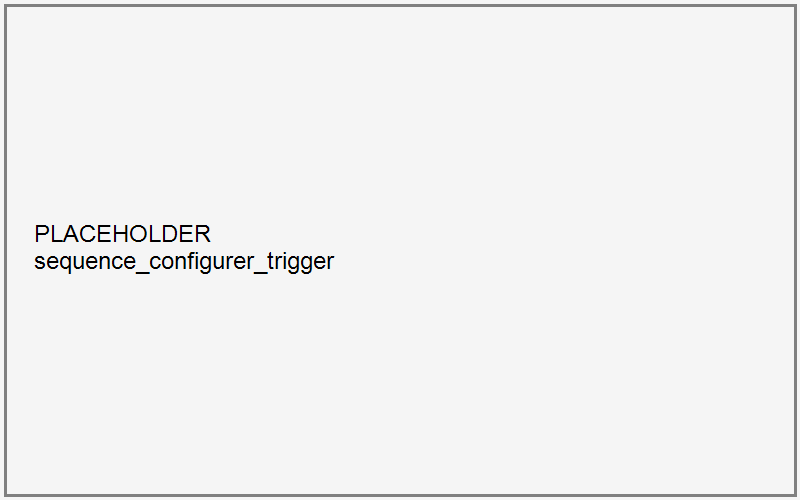
\includegraphics[width=15cm]{diagrammes/sequence_configurer_trigger.png}
    \caption{Diagramme de séquence — Configuration d'un déclencheur d'événement}
    \label{fig:seq-trigger}
\end{figure}

\subsection{Réalisation}

La création d'un déclencheur suit la logique suivante côté backend : validation de la propriété de l'application et du sujet Kafka par l'utilisateur courant (au travers de \texttt{UserContextService}), construction du manifeste \texttt{KafkaSource} référençant le sujet et le \textit{Broker} du tenant, construction du manifeste \texttt{Trigger} référençant le \textit{Broker} et l'URL interne du service Knative cible, puis application séquentielle de ces deux ressources sur le cluster.

\subsection{Difficultés rencontrées et solutions apportées}

L'implémentation initiale de ce module a présenté plusieurs anomalies de cohérence entre la base de données et l'état réel du cluster, mises en évidence lors d'un audit dédié du module Eventing/Kafka :

\begin{itemize}
    \item \textbf{Exceptions Fabric8 silencieusement absorbées} : certains appels de création de ressources capturaient les exceptions sans les propager ni les journaliser, laissant croire à un succès alors que la ressource n'avait pas été créée sur le cluster. \textit{Solution} : propagation et journalisation systématiques des erreurs Fabric8, avec échec explicite de l'opération côté API.
    \item \textbf{Espace de noms codé en dur} : certaines opérations référençaient un espace de noms fixe au lieu de celui du tenant courant. \textit{Solution} : résolution systématique de l'espace de noms à partir du contexte du tenant.
    \item \textbf{Ressources \texttt{Trigger} orphelines à la suppression} : la suppression d'une application ne supprimait pas systématiquement le \texttt{Trigger} associé, laissant une ressource orpheline sur le cluster. \textit{Solution} : suppression en cascade du \texttt{Trigger} et du \texttt{KafkaSource} lors de la suppression logique d'une application.
    \item \textbf{État de disponibilité non resynchronisé} : le statut de disponibilité d'un déclencheur n'était pas remis à jour après une reconfiguration. \textit{Solution} : resynchronisation explicite de l'état après chaque opération de création/mise à jour.
\end{itemize}

\subsection{Résultat obtenu}

Au terme de ce sprint, un client peut, en théorie via l'API backend, relier un sujet Kafka à l'une de ses applications de sorte que celle-ci soit automatiquement réveillée à la réception d'un message. Cette fonctionnalité ne sera exposée dans l'interface graphique du portail qu'à partir du Sprint 8 ; jusque-là, elle est validée par des appels directs à l'API (voir chapitre de validation).

\subsection{Conclusion du Sprint}

Ce sprint a permis de relier effectivement les deux briques serverless et événementielle du système, en identifiant et corrigeant plusieurs anomalies de cohérence critiques pour la fiabilité de la plateforme. Le sprint suivant s'attache désormais à sécuriser l'accès à l'ensemble de ces fonctionnalités.


\section{Sprint 4 : Authentification et sécurité}

\subsection{Introduction}

Ce sprint a pour objectif de mettre en place le mécanisme d'authentification et de contrôle d'accès de la plateforme, préalable indispensable avant d'exposer la moindre fonctionnalité applicative à un utilisateur final.

\subsection{Objectifs du Sprint}

\begin{itemize}
    \item Intégrer Keycloak comme fournisseur d'identité (OpenID Connect / OAuth2) pour l'authentification des utilisateurs.
    \item Définir le modèle de rôles (ADMIN, CLIENT\_ADMIN, MEMBER) et de permissions granulaires pour les MEMBER.
    \item Sécuriser l'API REST du backend en tant que serveur de ressources OAuth2 (validation des jetons JWT).
    \item Mettre en place un mécanisme d'authentification alternatif par clé d'API, destiné aux usages machine-à-machine (pipelines CI/CD).
    \item Mettre en place la synchronisation entre l'utilisateur authentifié auprès de Keycloak et l'entité utilisateur locale du backend.
\end{itemize}

\subsection{Sprint Backlog}

\begin{table}[!ht]
\begin{center}
     \begin{tabular}{|l{11cm}|l{3cm}|}
     \hline
     \textbf{User Story} & \textbf{Statut} \\
     \hline
     En tant qu'utilisateur, je veux me connecter à la plateforme avec mon compte & Réalisé \\
     \hline
     En tant que CLIENT\_ADMIN, je veux inviter des membres et leur attribuer des permissions & Réalisé \\
     \hline
     En tant que backend, je veux valider les jetons émis par Keycloak sur chaque requête & Réalisé \\
     \hline
     En tant que CLIENT\_ADMIN, je veux générer une clé d'API pour mon pipeline CI/CD & Réalisé \\
     \hline
     \end{tabular}
     \caption{Sprint Backlog — Sprint 4}
     \label{tab:sb-sprint4}
     \end{center}
\end{table}

\subsection{Diagramme de cas d'utilisation du Sprint}

\begin{figure}[h!]
 \centering
    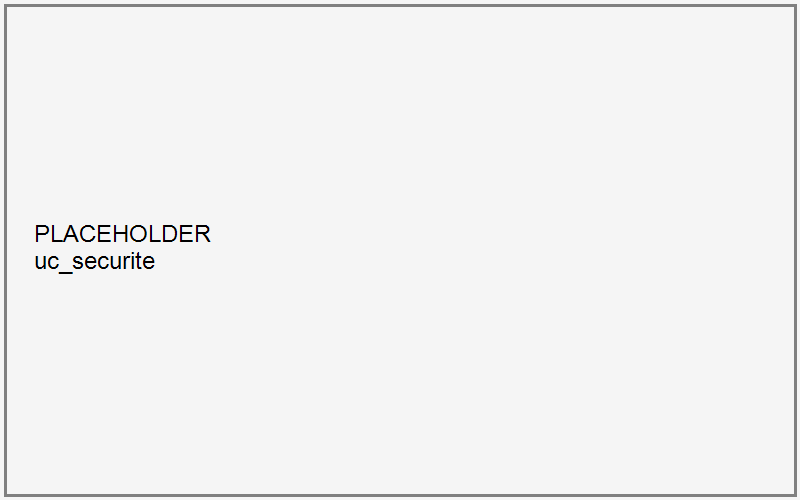
\includegraphics[width=12cm]{diagrammes/uc_securite.png}
    \caption{Diagramme de cas d'utilisation — Authentification et sécurité}
    \label{fig:uc-securite}
\end{figure}

\subsection{Présentation des composants développés}

\begin{itemize}
    \item \texttt{KeycloakJwtAuthConverter} : convertit les jetons JWT émis par Keycloak en objets d'authentification Spring Security, en extrayant les rôles applicatifs à partir de la revendication (\textit{claim}) \texttt{realm\_access.roles} du jeton.
    \item \texttt{UserSyncFilter} : filtre de sécurité créant, si nécessaire, l'entité \texttt{User} locale correspondant à l'utilisateur authentifié auprès de Keycloak lors de sa première requête, assurant la cohérence entre l'identité fédérée et le modèle de données interne.
    \item \texttt{UserRole} (énumération \texttt{ADMIN}, \texttt{CLIENT\_ADMIN}, \texttt{MEMBER}) et \texttt{Permission} : modèle de rôles et de permissions granulaires (déploiement, suppression d'application, gestion Kafka, gestion Eventing, consultation des journaux, consultation de la supervision, consultation et export de la facturation), vérifiées par le \texttt{PermissionService}.
    \item \texttt{UserContextService} : résout systématiquement l'identité \og effective \fg{} d'un appelant, en rattachant un \texttt{MEMBER} au compte de son \texttt{CLIENT\_ADMIN} pour toute opération portant sur la propriété d'une ressource.
    \item \texttt{ApiKeyService} / \texttt{ApiKeyFilter} : génération de clés d'API au format \texttt{plat\_<chaîne aléatoire>}, dont seul le hachage SHA-256 et un préfixe de 12 caractères sont conservés en base ; filtre de sécurité validant ces clés en amont de la chaîne Spring Security standard, pour un usage machine-à-machine (pipelines CI/CD).
\end{itemize}

\subsection{Description du cas d'utilisation « Se connecter à la plateforme »}

\subsubsection{Description textuelle}

\begin{table}[!ht]
\begin{center}
     \begin{tabular}{|l{3.5cm}|p{9cm}|}
     \hline
     \textbf{Nom} & Se connecter à la plateforme \\
     \hline
     \textbf{Acteur} & CLIENT\_ADMIN, MEMBER, ADMIN \\
     \hline
     \textbf{Pré-condition} & L'utilisateur possède un compte enregistré dans le royaume (\textit{realm}) Keycloak de la plateforme \\
     \hline
     \textbf{Scénario nominal} & 1. L'utilisateur saisit ses identifiants sur le portail. 2. Le portail échange ces identifiants contre un jeton JWT auprès de Keycloak. 3. Le portail joint ce jeton à chacune de ses requêtes vers le backend. 4. Le backend valide la signature et la validité du jeton, en extrait les rôles, et synchronise l'utilisateur local si besoin. 5. L'utilisateur accède aux fonctionnalités autorisées par son rôle et ses permissions. \\
     \hline
     \textbf{Post-condition} & Une session applicative authentifiée est établie côté portail. \\
     \hline
     \end{tabular}
     \caption{Description textuelle du cas d'utilisation « Se connecter à la plateforme »}
     \label{tab:uc-login}
     \end{center}
\end{table}

\subsubsection{Diagramme de séquence}

\begin{figure}[h!]
 \centering
    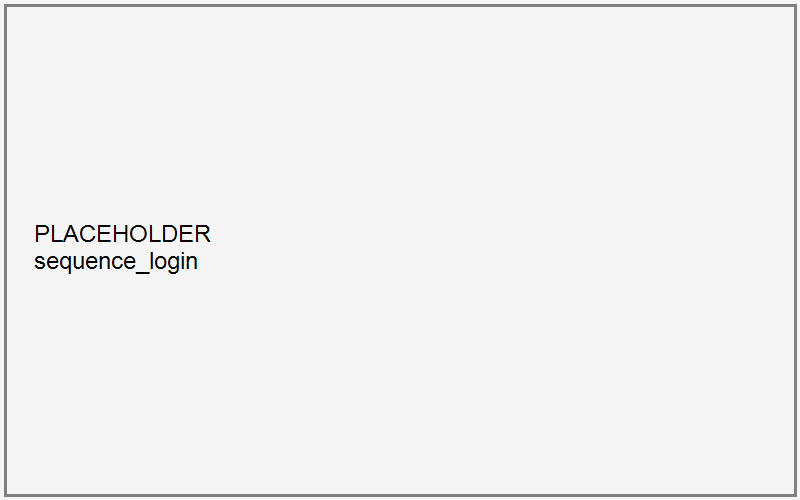
\includegraphics[width=15cm]{diagrammes/sequence_login.png}
    \caption{Diagramme de séquence — Authentification d'un utilisateur}
    \label{fig:seq-login}
\end{figure}

\subsection{Difficultés rencontrées et solutions apportées}

\begin{itemize}
    \item \textbf{Flux d'authentification implémenté côté portail} : l'échange des identifiants contre un jeton a été implémenté côté frontend selon le flux \textit{Resource Owner Password Credentials} (envoi direct du couple identifiant/mot de passe à Keycloak), plutôt que le flux \textit{Authorization Code avec PKCE}, recommandé pour les applications monopages car il évite toute manipulation du mot de passe par le code applicatif. Ce point a été identifié lors de l'audit de sécurité de la plateforme et \textbf{assumé comme un risque produit accepté} plutôt que corrigé dans le délai du projet ; il est repris explicitement dans les limites du chapitre de validation.
    \item \textbf{Jeton exposé dans les paramètres d'URL du flux de journaux en temps réel (SSE)} : le mécanisme natif \texttt{EventSource} du navigateur ne permettant pas l'envoi d'en-têtes HTTP personnalisés, le jeton d'authentification était initialement transmis en paramètre d'URL, avec un risque de fuite dans les journaux d'infrastructure (proxy, ingress). \textit{Solution} : migration vers la bibliothèque \texttt{@microsoft/fetch-event-source}, qui permet l'envoi du jeton dans l'en-tête \texttt{Authorization} standard, avec conservation d'un filtre de secours (\texttt{SseTokenFilter}) pour compatibilité.
    \item \textbf{Rôles Kubernetes (RBAC) sous-déclarés} : le rôle attribué au compte de service du backend ne couvrait pas initialement l'ensemble des ressources réellement manipulées (Knative, Eventing, Strimzi). \textit{Solution} : reconstruction du \texttt{ClusterRole} à partir des permissions effectivement nécessaires, vérifiées par la commande \texttt{kubectl auth can-i}.
\end{itemize}

\subsection{Résultat obtenu}

À l'issue de ce sprint, l'ensemble des fonctionnalités développées lors des sprints précédents et suivants sont protégées par une authentification centralisée via Keycloak, un modèle de rôles à trois niveaux et un système de permissions granulaires pour les membres d'équipe, ainsi qu'un mécanisme d'authentification alternatif par clé d'API pour les usages automatisés.

\subsection{Conclusion du Sprint}

Ce sprint a doté la plateforme d'un socle de sécurité indispensable avant l'ouverture de ses fonctionnalités métier à des utilisateurs réels. Le sprint suivant s'appuie directement sur ce socle pour livrer la première version exploitable de la gestion des applications.


\section{Sprint 5 : Gestion des applications et début du pipeline CI/CD Backend}

\subsection{Introduction}

Ce sprint constitue un jalon majeur du projet : il livre la première fonctionnalité complète et bout-en-bout accessible à un client de la plateforme — le déploiement d'une application — en s'appuyant sur l'ensemble des briques développées lors des sprints précédents (Knative Serving, authentification, permissions). Il initie en parallèle l'automatisation de la construction et du déploiement du backend lui-même.

\subsection{Objectifs du Sprint}

\begin{itemize}
    \item Développer le cycle de vie complet de gestion d'une application cliente : création, consultation, mise à jour, suppression logique, historique de révisions et retour à une révision antérieure.
    \item Garantir la réactivité de l'API en rendant le déploiement effectif sur le cluster asynchrone par rapport à la requête HTTP du client.
    \item Synchroniser en continu le statut de l'application en base de données avec son état réel sur le cluster.
    \item Mettre en place un premier pipeline Jenkins pour la construction, la publication et le déploiement automatisés du backend, en utilisant Kaniko pour la construction de l'image sans démon Docker privilégié.
\end{itemize}

\subsection{Sprint Backlog}

\begin{table}[!ht]
\begin{center}
     \begin{tabular}{|l{11cm}|l{3cm}|}
     \hline
     \textbf{User Story} & \textbf{Statut} \\
     \hline
     En tant que client, je veux déployer une application à partir d'une image Docker & Réalisé \\
     \hline
     En tant que client, je veux consulter l'état de mes applications en temps réel & Réalisé \\
     \hline
     En tant que client, je veux mettre à jour ou supprimer une application & Réalisé \\
     \hline
     En tant que client, je veux consulter l'historique des révisions et revenir à une version antérieure & Réalisé \\
     \hline
     En tant qu'exploitant, je veux que le backend soit reconstruit et redéployé automatiquement à chaque évolution du code & Réalisé \\
     \hline
     \end{tabular}
     \caption{Sprint Backlog — Sprint 5}
     \label{tab:sb-sprint5}
     \end{center}
\end{table}

\subsection{Diagramme de cas d'utilisation du Sprint}

\begin{figure}[h!]
 \centering
    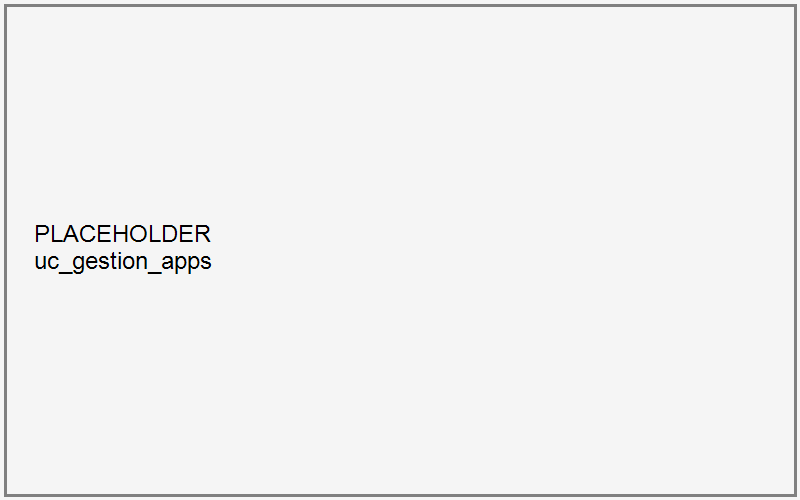
\includegraphics[width=12cm]{diagrammes/uc_gestion_apps.png}
    \caption{Diagramme de cas d'utilisation — Gestion des applications}
    \label{fig:uc-apps}
\end{figure}

\subsection{Présentation des composants développés}

\begin{itemize}
    \item \texttt{App} : entité métier représentant une application déployée, avec son statut (\texttt{DEPLOYING}, \texttt{RUNNING}, \texttt{FAILED}, \texttt{DELETED}, etc.), son image, son port et ses paramètres de mise à l'échelle.
    \item \texttt{AppController} / \texttt{AppService} : exposition de l'API REST de gestion des applications et implémentation de la logique métier (génération d'un nom de service unique compatible DNS, délégation de propriété MEMBER $\rightarrow$ CLIENT\_ADMIN).
    \item \texttt{AppDeploymentAsyncRunner} : composant dédié à l'exécution asynchrone du déploiement effectif sur le cluster, découplée du cycle de la requête HTTP entrante.
    \item \texttt{KnativeWatcher} : observateur Fabric8 surveillant en continu l'état des ressources Knative du cluster et répercutant les changements de statut sur l'entité \texttt{App} correspondante en base de données.
    \item \texttt{DeploymentLog} et \texttt{LogSseService} : journalisation des événements de cycle de vie d'une application et diffusion en temps réel au portail via un flux d'événements serveur (SSE).
\end{itemize}

\subsection{Description du cas d'utilisation « Déployer une application »}

\subsubsection{Description textuelle}

\begin{table}[!ht]
\begin{center}
     \begin{tabular}{|l{3.5cm}|p{9cm}|}
     \hline
     \textbf{Nom} & Déployer une application \\
     \hline
     \textbf{Acteur} & CLIENT\_ADMIN, MEMBER (avec permission de déploiement) \\
     \hline
     \textbf{Pré-condition} & L'utilisateur est authentifié et dispose de la permission \texttt{DEPLOY\_APP} \\
     \hline
     \textbf{Scénario nominal} & 1. L'utilisateur renseigne le formulaire de déploiement (nom, image, port, ressources, bornes de mise à l'échelle) et génère un nom de service unique. 2. L'entité \texttt{App} est créée avec le statut \texttt{DEPLOYING} et un \texttt{DeploymentLog} est émis. 3. Le backend répond immédiatement, puis déclenche de manière asynchrone la création de la ressource Knative correspondante. 4. Le statut de l'application est mis à jour en temps réel à mesure que Knative provisionne le service. \\
     \hline
     \textbf{Scénario étendu} & Si l'utilisateur a activé l'onglet « Kafka Trigger » du formulaire (sujet Kafka + éventuel type de filtre), et une fois le déploiement Knative réussi, le backend crée automatiquement, dans la même exécution asynchrone, un \texttt{KafkaSource} et un \texttt{Trigger} pointant vers l'URL du service qui vient d'être déployé — sans étape manuelle supplémentaire de l'utilisateur. \\
     \hline
     \textbf{Post-condition} & L'application est déployée et accessible (et, le cas échéant, câblée à son sujet Kafka), ou son statut reflète l'échec du déploiement. \\
     \hline
     \end{tabular}
     \caption{Description textuelle du cas d'utilisation « Déployer une application »}
     \label{tab:uc-deploy}
     \end{center}
\end{table}

\subsubsection{Diagramme de séquence}

Le diagramme de séquence détaillé de ce cas d'utilisation reprend et détaille, au niveau des classes du backend introduites dans ce sprint, le processus déjà présenté de manière transverse à la figure~\ref{fig:seq-deploiement} du chapitre 2 (Analyse et spécification des besoins).

\begin{figure}[h!]
 \centering
    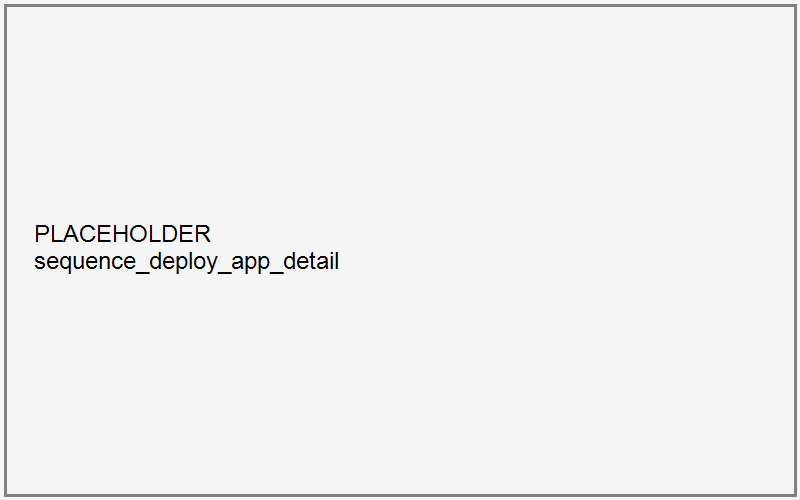
\includegraphics[width=15.5cm,height=21cm]{diagrammes/sequence_deploy_app_detail.png}
    \caption{Diagramme de séquence détaillé — Déployer une application}
    \label{fig:seq-deploy-detail}
\end{figure}

\subsection{Présentation de la réalisation}

Le formulaire de déploiement et la vue de détail d'une application (statut en temps réel, journaux, historique de révisions) sont accessibles depuis le portail client à partir du Sprint 8, lorsque l'interface graphique correspondante est livrée. À ce stade du projet (fin de Sprint 5), ces fonctionnalités ont été validées par des appels directs à l'API REST (voir captures d'écran de tests API au chapitre de validation).

\subsubsection{Intégration Kafka automatique au moment du déploiement}

Au-delà du scénario nominal, \texttt{AppDeploymentAsyncRunner} implémente un second chemin, optionnel, qui anticipe sur la fonctionnalité développée au Sprint 6 : si la requête de déploiement porte un indicateur \texttt{kafkaEnabled} et l'identifiant d'un sujet Kafka existant, le backend crée automatiquement, \textbf{juste après le succès du déploiement Knative et dans la même exécution asynchrone}, un \texttt{KafkaSource} puis un \texttt{Trigger} pointant vers l'URL du service qui vient d'être déployé. Ce chemin se distingue du flux manuel de configuration d'un déclencheur présenté au Sprint 6 sur un point technique important : l'URL transmise en paramètre \texttt{action} au \texttt{Trigger} est ici directement celle que \texttt{KnativeService.deploy()} vient de renvoyer pour l'application en cours de création — l'égalité entre le nom d'abonné du \texttt{Trigger} et le service réellement déployé est donc garantie par construction, alors qu'elle dépend, dans le flux manuel du Sprint 6, de la valeur fournie librement par l'appelant. En cas d'échec du déploiement Knative, cette étape n'est jamais exécutée : aucune ressource d'Eventing n'est créée pour une application qui n'a pas démarré.

\subsection{Le pipeline CI/CD Backend}

Un premier pipeline Jenkins est mis en place pour le backend, structuré selon les étapes suivantes : récupération du code source (avec réessai automatique en cas d'échec transitoire), compilation Maven (\texttt{mvn clean package}), construction de l'image de conteneur par \textbf{Kaniko} — outil permettant de construire une image Docker à l'intérieur même du pod Jenkins, sans nécessiter de démon Docker privilégié — publication de l'image sur Docker Hub, puis mise à jour de l'image du déploiement Kubernetes du backend (\texttt{kubectl set image}) suivie de la vérification du succès du déploiement (\texttt{kubectl rollout status}).

\subsection{Difficultés rencontrées et solutions apportées}

\begin{itemize}
    \item \textbf{Déploiement \og asynchrone \fg{} en réalité bloquant} : la méthode de création d'une application invoquait sa méthode de déploiement asynchrone directement sur \texttt{this}, contournant ainsi le mécanisme de proxy AOP de Spring responsable de l'exécution effective en tâche de fond. La requête HTTP restait donc bloquée jusqu'à 60 secondes, le temps que la boucle de tentative de construction de l'URL du service Knative aboutisse. \textit{Solution} : refactorisation en confiant l'appel asynchrone à un composant dédié (\texttt{AppDeploymentAsyncRunner}), invoqué depuis l'extérieur de la classe \texttt{AppService} afin que le proxy Spring soit correctement sollicité.
    \item \textbf{Corruption de la machine virtuelle Java par Kaniko} : l'exécution de Kaniko purgeant le répertoire temporaire partagé du conteneur Jenkins perturbait le mécanisme interne de création de processus fils de la JVM (\texttt{jspawnhelper}), provoquant des échecs aléatoires de constructions ultérieures. \textit{Solution} : ajout des options Kaniko \texttt{--use-new-run} et \texttt{--snapshot-mode=redo}, et redémarrage sécurisé (\texttt{safeRestart}) de Jenkins après chaque exécution du pipeline, quel que soit son résultat.
    \item \textbf{Flux SSE des journaux incohérent selon le rôle} : le canal de diffusion des journaux en temps réel indexait les abonnements par nom d'utilisateur, alors que les événements étaient émis avec l'identifiant utilisateur effectif (après résolution MEMBER $\rightarrow$ CLIENT\_ADMIN), provoquant une absence de réception des journaux, en particulier pour les membres d'équipe. \textit{Solution} : alignement de la clé d'indexation des abonnements sur l'identifiant utilisateur effectif.
\end{itemize}

\subsection{Résultat obtenu}

Au terme de ce sprint, la plateforme dispose d'un cycle de vie de gestion des applications complet et fonctionnel, exploitable par l'API REST, avec un déploiement réellement asynchrone, un suivi de statut en temps réel, et un pipeline d'intégration continue opérationnel pour le backend lui-même.

\subsection{Conclusion du Sprint}

Ce sprint clôt la Release 1 sur un jalon fonctionnel majeur : la chaîne complète de déploiement d'une application, de la requête utilisateur jusqu'à son exécution effective sur le cluster, est désormais opérationnelle et sécurisée. La Release 2, objet du chapitre suivant, vient enrichir cette base par la gestion applicative de Kafka et de l'Eventing côté backend, ainsi que par la supervision de la plateforme.

\section{Conclusion}

La Release 1 a transformé les briques d'infrastructure isolées de la Release 0 en une plateforme applicative cohérente : sécurisation des accès via Keycloak et un modèle de permissions granulaires, mise en relation opérationnelle de Kafka et de Knative Serving via Knative Eventing, et livraison du cas d'utilisation central de la plateforme — le déploiement d'une application — accompagné du démarrage de son propre pipeline d'intégration continue. Plusieurs anomalies de cohérence et de sécurité ont été identifiées et corrigées au cours de cette release, illustrant une démarche itérative de durcissement progressif de la plateforme, poursuivie dans les releases suivantes.

\chapter*{chapitre 5}
\markboth{Chapitre 5 }{5 Release 2 : Services avancés} %pour afficher l'entete
 \addcontentsline{toc}{chapter}{5 Release 2 : Services avancés}

\textbf{\Huge Release 2 : Services avancés}

\setcounter{chapter}{5}
\setcounter{section}{0}

\section{Introduction}

La Release 1 a livré le cas d'utilisation central de la plateforme — le déploiement sécurisé d'une application — ainsi que les briques techniques de Knative Eventing, exploitées jusqu'ici uniquement au niveau du backend. La Release 2 a pour objectif d'exposer ces briques comme de véritables services applicatifs accessibles aux clients (gestion de Kafka et de l'Eventing au travers de l'API), et de doter la plateforme des capacités de supervision nécessaires à son exploitation en conditions réelles : métriques, journaux et détection automatique d'anomalies. Elle regroupe le Sprint 6 et le Sprint 7.


\section{Sprint 6 : Gestion Kafka et Eventing côté Backend}

\subsection{Introduction}

Ce sprint a pour objectif de transformer les capacités techniques de gestion de Kafka (Sprint 2) et de Knative Eventing (Sprint 3), jusque-là exploitées uniquement en interne par le backend, en véritables services applicatifs exposés aux clients au travers de l'API REST, avec les contrôles d'appartenance et de permission requis par le modèle multi-tenant.

\subsection{Objectifs du Sprint}

\begin{itemize}
    \item Exposer, au travers de l'API REST, les opérations de création, de consultation et de suppression des sujets Kafka d'un client.
    \item Exposer, au travers de l'API REST, les opérations de configuration des déclencheurs d'événement (association d'un sujet Kafka à une application).
    \item Garantir que ces opérations respectent strictement l'isolation multi-tenant, y compris pour les utilisateurs de type MEMBER.
\end{itemize}

\subsection{Sprint Backlog}

\begin{table}[!ht]
\begin{center}
     \begin{tabular}{|l{11cm}|l{3cm}|}
     \hline
     \textbf{User Story} & \textbf{Statut} \\
     \hline
     En tant que client, je veux créer un sujet Kafka pour mon compte & Réalisé \\
     \hline
     En tant que client, je veux lister et supprimer mes sujets Kafka & Réalisé \\
     \hline
     En tant que client, je veux configurer un déclencheur reliant un sujet à une application & Réalisé \\
     \hline
     En tant que MEMBER, je veux que mes actions Kafka/Eventing soient rattachées au bon compte client & Réalisé (après correction) \\
     \hline
     \end{tabular}
     \caption{Sprint Backlog — Sprint 6}
     \label{tab:sb-sprint6}
     \end{center}
\end{table}

\subsection{Diagramme de cas d'utilisation du Sprint}

\begin{figure}[h!]
 \centering
    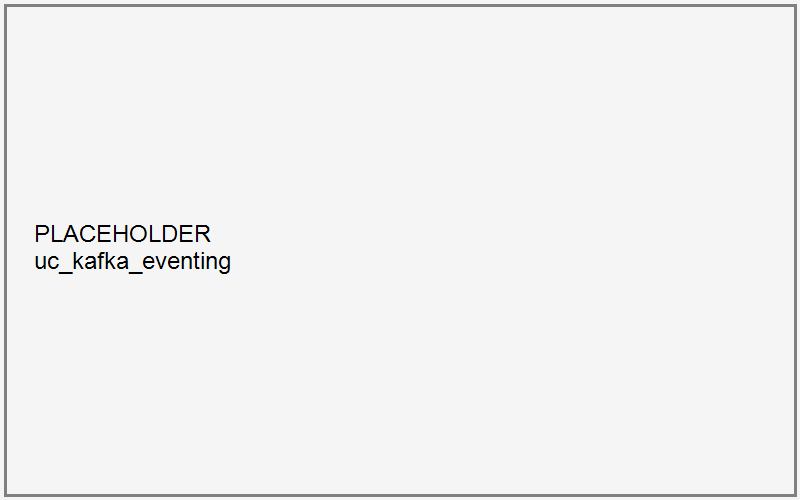
\includegraphics[width=12cm]{diagrammes/uc_kafka_eventing.png}
    \caption{Diagramme de cas d'utilisation — Gestion Kafka et Eventing}
    \label{fig:uc-kafka}
\end{figure}

\subsection{Présentation des composants développés}

\begin{itemize}
    \item \texttt{KafkaController} : expose les points d'accès REST de création, de listing et de suppression des sujets Kafka d'un tenant, en s'appuyant sur \texttt{KafkaService} (Sprint 2) pour l'interaction avec la ressource \texttt{KafkaTopic}.
    \item \texttt{EventingController} : expose les points d'accès REST de configuration des déclencheurs (\texttt{Trigger}/\texttt{KafkaSource}), en s'appuyant sur \texttt{EventingService} (Sprint 3).
    \item Intégration systématique de \texttt{UserContextService} dans ces deux contrôleurs, afin de garantir que toute opération est rattachée à l'identité effective de l'appelant (compte CLIENT\_ADMIN, y compris lorsque l'appelant est un MEMBER).
\end{itemize}

\subsection{Description du cas d'utilisation « Créer un sujet Kafka »}

\subsubsection{Description textuelle}

\begin{table}[!ht]
\begin{center}
     \begin{tabular}{|l{3.5cm}|p{9cm}|}
     \hline
     \textbf{Nom} & Créer un sujet Kafka \\
     \hline
     \textbf{Acteur} & CLIENT\_ADMIN, MEMBER (avec permission de gestion Kafka) \\
     \hline
     \textbf{Pré-condition} & L'utilisateur est authentifié et dispose de la permission requise \\
     \hline
     \textbf{Scénario nominal} & 1. L'utilisateur soumet un nom de sujet. 2. Le backend résout l'identité effective (compte propriétaire) de l'appelant. 3. Le backend crée la ressource \texttt{KafkaTopic} rattachée au cluster Kafka du tenant. 4. Le sujet créé est renvoyé à l'utilisateur et devient disponible pour la configuration de déclencheurs. \\
     \hline
     \textbf{Post-condition} & Le sujet est disponible pour publication/consommation et pour association à une application via un Trigger. \\
     \hline
     \end{tabular}
     \caption{Description textuelle du cas d'utilisation « Créer un sujet Kafka »}
     \label{tab:uc-create-topic}
     \end{center}
\end{table}

\subsubsection{Diagramme de séquence}

\begin{figure}[h!]
 \centering
    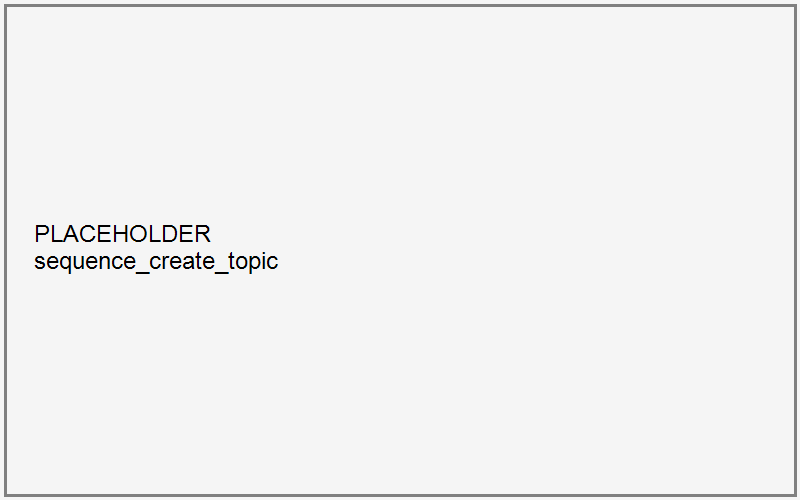
\includegraphics[width=14cm]{diagrammes/sequence_create_topic.png}
    \caption{Diagramme de séquence — Création d'un sujet Kafka}
    \label{fig:seq-create-topic}
\end{figure}

\subsection{Difficultés rencontrées et solutions apportées}

\begin{itemize}
    \item \textbf{Isolation multi-tenant rompue pour les membres d'équipe} : les contrôleurs Kafka et Eventing utilisaient initialement directement l'identifiant d'authentification brut (\texttt{auth.getName()}) au lieu de l'identifiant effectif résolu par \texttt{UserContextService}. Un utilisateur MEMBER pouvait ainsi voir ses ressources Kafka/Eventing rattachées à son propre identifiant plutôt qu'à celui de son compte CLIENT\_ADMIN, cassant le modèle de délégation de propriété établi au Sprint 4 et pouvant conduire à des incohérences d'accès entre membres d'une même équipe. \textit{Solution} : remplacement systématique de ces appels par la résolution via \texttt{UserContextService}, alignant ce module sur le reste du backend.
\end{itemize}

\subsection{Résultat obtenu}

À l'issue de ce sprint, un client peut créer, consulter et supprimer ses sujets Kafka, et configurer des déclencheurs d'événement reliant ses sujets à ses applications, directement au travers de l'API REST, avec une isolation multi-tenant correctement appliquée y compris pour les membres d'équipe. L'exposition de ces fonctionnalités dans l'interface graphique du portail interviendra au Sprint 8.

\subsection{Conclusion du Sprint}

Ce sprint a complété le triptyque applicatif Serverless/Kafka/Eventing initié dès la Release 0, en le rendant pleinement exploitable par les clients au travers de l'API. Le sprint suivant s'attache désormais à doter la plateforme de capacités de supervision, indispensables à son exploitation.


\section{Sprint 7 : Monitoring, métriques et gestion des logs}

\subsection{Introduction}

Ce sprint a pour objectif de doter la plateforme des capacités d'observabilité nécessaires à son exploitation : consultation des journaux applicatifs et de déploiement par les clients, supervision de l'état du cluster par l'équipe d'exploitation, et détection automatique des applications en échec récurrent.

\subsection{Objectifs du Sprint}

\begin{itemize}
    \item Exposer aux clients les journaux de déploiement et les journaux applicatifs (logs des conteneurs) de leurs applications, en temps réel.
    \item Intégrer Prometheus pour la collecte des métriques du backend et des révisions Knative.
    \item Exposer à l'équipe d'exploitation une vue de supervision du cluster (nœuds, alertes actives, usage par tenant) au travers de la console d'administration.
    \item Mettre en place une détection automatique des redémarrages en boucle (\textit{crash loops}) des applications clientes.
\end{itemize}

\subsection{Sprint Backlog}

\begin{table}[!ht]
\begin{center}
     \begin{tabular}{|l{11cm}|l{3cm}|}
     \hline
     \textbf{User Story} & \textbf{Statut} \\
     \hline
     En tant que client, je veux consulter en temps réel les journaux de mon application & Réalisé \\
     \hline
     En tant qu'exploitant, je veux que les métriques du backend soient collectées par Prometheus & Réalisé (avec anomalie identifiée) \\
     \hline
     En tant qu'exploitant, je veux visualiser l'état des nœuds et les alertes actives du cluster & Réalisé \\
     \hline
     En tant qu'exploitant, je veux être informé automatiquement d'une application en boucle de redémarrage & Réalisé \\
     \hline
     \end{tabular}
     \caption{Sprint Backlog — Sprint 7}
     \label{tab:sb-sprint7}
     \end{center}
\end{table}

\subsection{Diagramme de cas d'utilisation du Sprint}

\begin{figure}[h!]
 \centering
    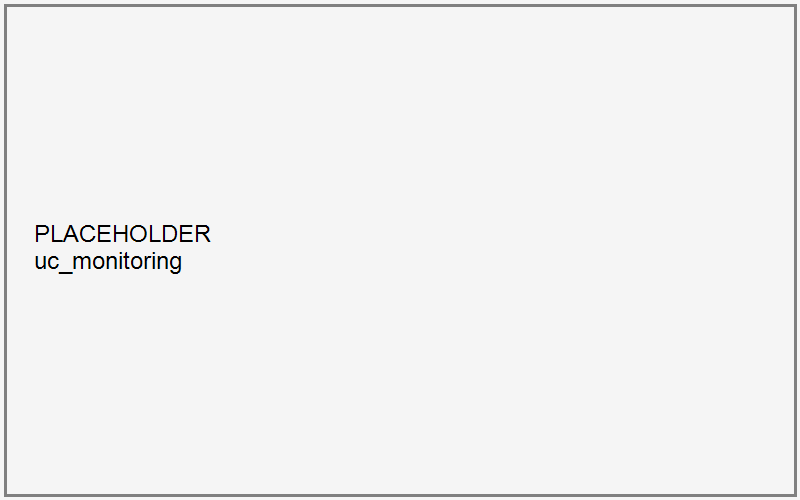
\includegraphics[width=12cm]{diagrammes/uc_monitoring.png}
    \caption{Diagramme de cas d'utilisation — Monitoring et logs}
    \label{fig:uc-monitoring}
\end{figure}

\subsection{Présentation des composants développés}

\begin{itemize}
    \item \texttt{PodLogService} / \texttt{PodLogStreamService} : récupération et diffusion en flux continu des journaux d'un pod applicatif via l'API Kubernetes.
    \item \texttt{LogSseService} : hub de diffusion en temps réel (Server-Sent Events) des journaux de déploiement et applicatifs vers le portail client.
    \item \textbf{Prometheus / Micrometer} : exposition des métriques du backend via le point d'accès \texttt{/actuator/prometheus}, collecte configurée par une ressource \texttt{ServiceMonitor} ; collecte des métriques par révision Knative (latence, concurrence) via une ressource \texttt{PodMonitor} ciblant le conteneur \textit{queue-proxy} de chaque révision.
    \item \texttt{AlertmanagerService} : interrogation de l'API d'Alertmanager pour remonter les alertes actives dans la console d'administration.
    \item \texttt{CrashLoopScheduler} : tâche planifiée interrogeant périodiquement l'état des pods des applications clientes et signalant, avec une période de répit (\textit{cooldown}) d'une heure par application, celles dépassant un seuil de cinq redémarrages.
    \item \texttt{AdminController} (volet supervision) : expose à la console d'administration l'état des nœuds, des espaces de noms, des pods et des alertes du cluster.
\end{itemize}

\subsection{Description du cas d'utilisation « Consulter les journaux d'une application »}

\subsubsection{Description textuelle}

\begin{table}[!ht]
\begin{center}
     \begin{tabular}{|l{3.5cm}|p{9cm}|}
     \hline
     \textbf{Nom} & Consulter les journaux d'une application \\
     \hline
     \textbf{Acteur} & CLIENT\_ADMIN, MEMBER (avec permission de consultation des journaux) \\
     \hline
     \textbf{Pré-condition} & L'application appartient au compte de l'utilisateur (ou de son CLIENT\_ADMIN) \\
     \hline
     \textbf{Scénario nominal} & 1. L'utilisateur ouvre la vue des journaux de son application. 2. Le portail établit une connexion en flux continu vers le backend. 3. Le backend récupère les journaux du conteneur applicatif du pod concerné et les diffuse en temps réel. 4. L'utilisateur visualise les journaux au fil de leur émission. \\
     \hline
     \textbf{Post-condition} & L'utilisateur dispose d'une vue à jour de l'activité de son application. \\
     \hline
     \end{tabular}
     \caption{Description textuelle du cas d'utilisation « Consulter les journaux d'une application »}
     \label{tab:uc-logs}
     \end{center}
\end{table}

\subsubsection{Diagramme de séquence}

\begin{figure}[h!]
 \centering
    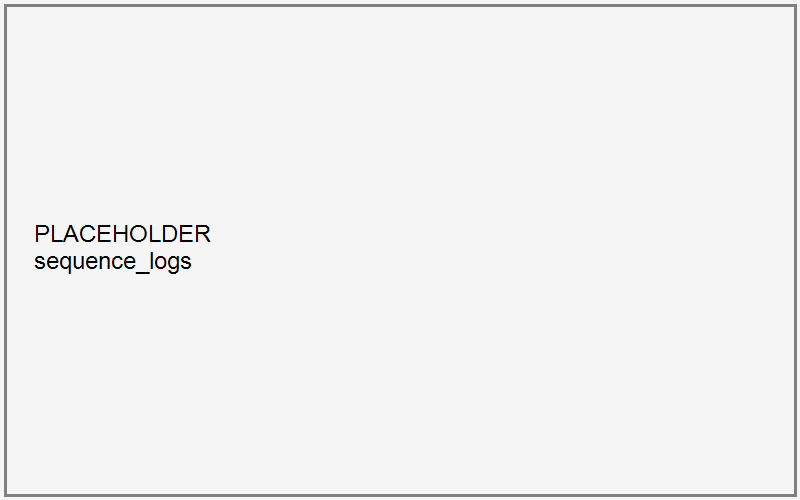
\includegraphics[width=14cm]{diagrammes/sequence_logs.png}
    \caption{Diagramme de séquence — Consultation des journaux en temps réel}
    \label{fig:seq-logs}
\end{figure}

\subsection{Difficultés rencontrées et solutions apportées}

\begin{itemize}
    \item \textbf{Récupération de journaux vide sur les pods Knative} : un pod géré par Knative Serving contient systématiquement deux conteneurs (le conteneur applicatif \texttt{user-container} et le conteneur \textit{sidecar} \texttt{queue-proxy}) ; l'appel initial de récupération des journaux ne précisait pas le conteneur cible et retournait donc un résultat ambigu ou vide. \textit{Solution} : ciblage explicite du conteneur \texttt{user-container} dans les appels Fabric8 de récupération de journaux.
    \item \textbf{Métriques du backend jamais collectées par Prometheus} : les ressources \texttt{ServiceMonitor} et les règles d'alerte du backend portaient une étiquette (\texttt{release: prometheus}) ne correspondant pas au sélecteur réellement configuré sur l'opérateur Prometheus du cluster (\texttt{release: monitoring-stack}), de sorte que les métriques applicatives du backend n'étaient, en pratique, jamais scrutées. Cette anomalie a été identifiée lors de l'audit de la plateforme ; sa correction n'était \textbf{pas encore confirmée en production} au moment de la rédaction de ce mémoire et est reprise comme limite au chapitre de validation.
    \item \textbf{Métrique de requêtes par seconde erronée} : le tableau de bord de supervision du cluster affichait initialement une valeur nulle pour le débit de requêtes, en raison de l'utilisation d'un nom de métrique Prometheus incorrect (\texttt{activator\_request\_count} au lieu de \texttt{revision\_request\_count}). \textit{Solution} : correction du nom de métrique interrogé.
\end{itemize}

\subsection{Résultat obtenu}

Au terme de cette release, la plateforme permet aux clients de suivre en temps réel l'activité de leurs applications, et à l'équipe d'exploitation de superviser l'état global du cluster et d'être alertée automatiquement en cas de dysfonctionnement récurrent d'une application, avec une anomalie de collecte de métriques backend identifiée et non encore définitivement corrigée.

\subsection{Conclusion du Sprint}

Ce sprint clôt la Release 2. La plateforme dispose désormais de l'ensemble des capacités de gestion applicative (applications, Kafka, Eventing) et de supervision nécessaires à son exploitation. La Release 3, objet du chapitre suivant, se concentre sur la livraison de l'interface graphique exposant l'ensemble de ces fonctionnalités aux utilisateurs finaux, ainsi que sur l'industrialisation du pipeline CI/CD.

\section{Conclusion}

La Release 2 a consolidé la couche de services de la plateforme en exposant, de manière sécurisée et isolée par tenant, la gestion de Kafka et de l'Eventing, et en dotant le système de capacités d'observabilité indispensables à son exploitation réelle. Comme pour les releases précédentes, plusieurs anomalies concrètes ont été identifiées et corrigées, à l'exception notable de la collecte de métriques du backend, dont la correction reste à confirmer — un point traité en toute transparence dans le chapitre de validation.

\chapter*{chapitre 6}
\markboth{Chapitre 6 }{6 Release 3 : Interface utilisateur et industrialisation} %pour afficher l'entete
 \addcontentsline{toc}{chapter}{6 Release 3 : Interface utilisateur et industrialisation}

\textbf{\Huge Release 3 : Interface utilisateur et industrialisation}

\setcounter{chapter}{6}
\setcounter{section}{0}

\section{Introduction}

Les releases précédentes ont livré l'ensemble des services backend de la plateforme : déploiement d'applications, gestion de Kafka et de l'Eventing, sécurité, supervision. Jusqu'ici, ces fonctionnalités n'étaient validées qu'au travers d'appels directs à l'API REST. La Release 3, objet de ce chapitre, a pour objectif de rendre ces fonctionnalités accessibles à un utilisateur final au travers de deux interfaces web (portail client et console d'administration), puis de consolider et d'industrialiser les chaînes d'intégration continue de l'ensemble des composants de la plateforme. Elle regroupe le Sprint 8, le Sprint 9 et le Sprint 10.


\section{Sprint 8 : Développement du Frontend}

\subsection{Introduction}

Ce sprint a pour objectif de livrer une première version fonctionnelle des deux applications web de la plateforme — le portail client et la console d'administration — couvrant les cas d'utilisation développés côté backend depuis la Release 1.

\subsection{Objectifs du Sprint}

\begin{itemize}
    \item Mettre en place le socle technique commun des deux applications React (authentification via Keycloak, gestion des thèmes, notifications, mise en page générale).
    \item Développer les pages principales du portail client : tableau de bord, liste des applications, formulaire de déploiement, détail d'une application (statut, journaux, révisions).
    \item Développer les pages principales de la console d'administration : tableau de bord administrateur, gestion des clients, supervision du cluster.
    \item Mettre en place un premier pipeline Jenkins pour la construction et le déploiement du portail client et de la console d'administration.
\end{itemize}

\subsection{Sprint Backlog}

\begin{table}[!ht]
\begin{center}
     \begin{tabular}{|l{11cm}|l{3cm}|}
     \hline
     \textbf{User Story} & \textbf{Statut} \\
     \hline
     En tant qu'utilisateur, je veux me connecter via une interface web & Réalisé \\
     \hline
     En tant que client, je veux déployer une application depuis un formulaire graphique & Réalisé \\
     \hline
     En tant que client, je veux visualiser mes applications et leur statut & Réalisé \\
     \hline
     En tant qu'exploitant, je veux disposer d'une console d'administration séparée du portail client & Réalisé \\
     \hline
     En tant qu'exploitant, je veux que les frontends soient construits et déployés automatiquement & Réalisé \\
     \hline
     \end{tabular}
     \caption{Sprint Backlog — Sprint 8}
     \label{tab:sb-sprint8}
     \end{center}
\end{table}

\subsection{Diagramme de cas d'utilisation du Sprint}

Ce sprint ne développe pas de nouveaux cas d'utilisation métier : il expose graphiquement des cas d'utilisation déjà spécifiés et réalisés côté backend lors des releases précédentes (\og Déployer une application \fg{}, \og Consulter les journaux \fg{}, \og Créer un sujet Kafka \fg{}, etc. — voir figure~\ref{fig:uc-global} du chapitre d'analyse des besoins). Aucun diagramme de cas d'utilisation supplémentaire n'est donc introduit ici.

\subsection{Présentation des composants développés}

\paragraph{Portail client (\texttt{web-portal}).} Application React (Vite, React Router, MUI, Tailwind CSS) structurée autour d'un contexte d'authentification (\texttt{AuthContext}) s'appuyant sur \texttt{keycloak-js}, d'un client API centralisé (\texttt{api/client.js}) et d'un module de connexion aux flux d'événements serveur (\texttt{api/sse.js}). Les pages principales livrées à ce stade sont : \texttt{Dashboard} (vue d'ensemble du compte), \texttt{AppsList} (liste des applications), \texttt{DeployApp} (formulaire de déploiement), \texttt{AppDetails} (détail, statut temps réel, journaux, révisions), \texttt{Login}/\texttt{Register}.

\paragraph{Console d'administration (\texttt{admin-console}).} Application React de structure similaire, dont les pages principales livrées à ce stade sont : \texttt{AdminDashboard} (vue d'ensemble de la plateforme), \texttt{AdminClients} (gestion des comptes clients), \texttt{ClusterManagement} (supervision du cluster : nœuds, alertes, espaces de noms).

\subsection{Présentation de la réalisation}

Les figures~\ref{fig:capture-deploy} et~\ref{fig:capture-cluster} illustrent respectivement le formulaire de déploiement d'une application sur le portail client, et la vue de supervision du cluster sur la console d'administration.

\begin{figure}[h!]
 \centering
    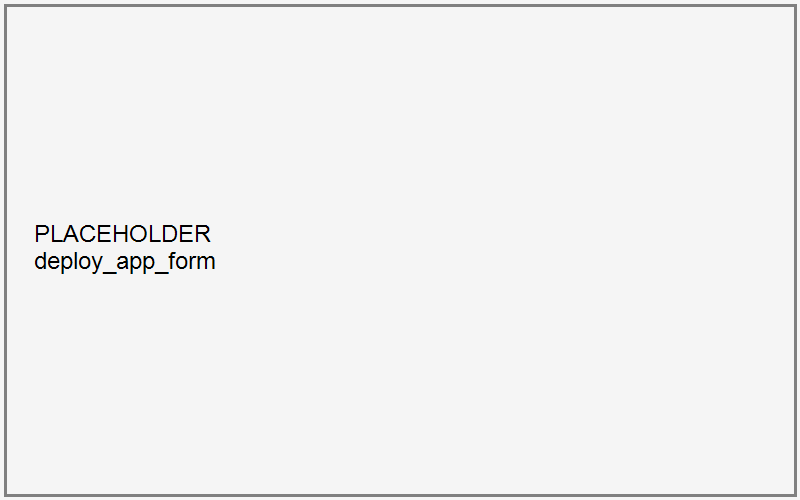
\includegraphics[width=13cm]{captures/deploy_app_form.png}
    \caption{Capture d'écran — Formulaire de déploiement d'une application}
    \label{fig:capture-deploy}
\end{figure}

\begin{figure}[h!]
 \centering
    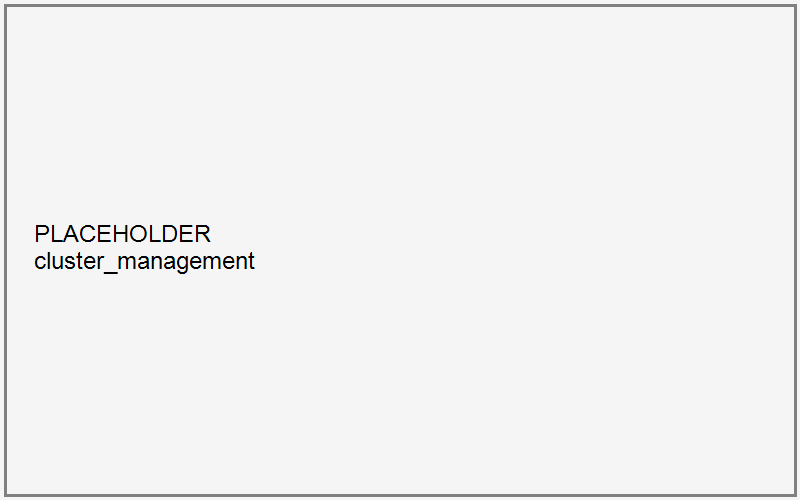
\includegraphics[width=13cm]{captures/cluster_management.png}
    \caption{Capture d'écran — Supervision du cluster (console d'administration)}
    \label{fig:capture-cluster}
\end{figure}

\subsection{Le pipeline CI/CD Frontend}

Deux pipelines Jenkins distincts (un pour le portail client, un pour la console d'administration) sont mis en place, reprenant le même squelette que le pipeline backend du Sprint 5 : construction (\texttt{npm run build}) produisant les fichiers statiques, construction de l'image de conteneur (Nginx servant ces fichiers statiques) via Kaniko, publication sur Docker Hub, puis mise à jour du déploiement Kubernetes correspondant.

\subsection{Difficultés rencontrées et solutions apportées}

\begin{itemize}
    \item \textbf{Duplication de code entre les deux applications React} : les deux applications partagent une quinzaine de fichiers quasi identiques (contexte d'authentification, client API, thème, composants de mise en page) sans outillage de monorepo ni paquet partagé. Cette duplication, assumée faute de temps disponible dans le sprint pour la refactoriser, est identifiée comme dette technique et reprise dans les limites du chapitre de validation.
    \item \textbf{Pipelines frontend moins robustes que le pipeline backend} : les pipelines du portail client et de la console d'administration ne reprennent pas l'ensemble des mécanismes de fiabilisation mis en place pour le pipeline backend au Sprint 5 (options anti-corruption de Kaniko, redémarrage systématique de Jenkins). \textit{Solution partielle} : ce point est traité au Sprint 10, consacré à l'optimisation du pipeline CI/CD.
\end{itemize}

\subsection{Résultat obtenu}

Au terme de ce sprint, les fonctionnalités principales de déploiement et de supervision d'applications, développées côté backend depuis la Release 1, sont accessibles au travers d'interfaces graphiques fonctionnelles, construites et déployées automatiquement.

\subsection{Conclusion du Sprint}

Ce sprint a rendu la plateforme utilisable de bout en bout par un utilisateur final pour son cas d'usage principal. Le sprint suivant complète l'interface graphique par les fonctionnalités restantes (Kafka, Eventing, facturation, équipe, audit).


\section{Sprint 9 : Finalisation du Frontend}

\subsection{Introduction}

Ce sprint a pour objectif de compléter l'interface graphique des deux applications avec l'ensemble des fonctionnalités développées côté backend lors des Releases 1 et 2, mais non encore exposées graphiquement à l'issue du Sprint 8.

\subsection{Objectifs du Sprint}

\begin{itemize}
    \item Développer les pages de gestion Kafka et de configuration de l'Eventing sur le portail client.
    \item Développer les pages de facturation, de gestion d'équipe et de paramètres du compte sur le portail client.
    \item Développer les pages de facturation globale, de journal d'audit et de gestion des utilisateurs sur la console d'administration.
    \item Mettre en place une page de statut public de la plateforme.
\end{itemize}

\subsection{Sprint Backlog}

\begin{table}[!ht]
\begin{center}
     \begin{tabular}{|l{11cm}|l{3cm}|}
     \hline
     \textbf{User Story} & \textbf{Statut} \\
     \hline
     En tant que client, je veux gérer mes sujets Kafka depuis le portail & Réalisé \\
     \hline
     En tant que client, je veux configurer des déclencheurs d'événement depuis le portail & Réalisé \\
     \hline
     En tant que client, je veux consulter ma facturation et gérer mon équipe & Réalisé \\
     \hline
     En tant qu'exploitant, je veux consulter le journal d'audit et la facturation globale & Réalisé \\
     \hline
     \end{tabular}
     \caption{Sprint Backlog — Sprint 9}
     \label{tab:sb-sprint9}
     \end{center}
\end{table}

\subsection{Présentation des composants développés}

\paragraph{Portail client.} Ajout des pages \texttt{KafkaTopics} et \texttt{Eventing} (gestion visuelle des sujets et des déclencheurs, cf. Sprint 6), \texttt{LogsView} et \texttt{Monitoring} (visualisation détaillée des journaux et métriques, cf. Sprint 7), \texttt{Billing} (facturation du compte, cf. modèle de facturation présenté au chapitre de modélisation), \texttt{Team} (gestion des membres et de leurs permissions, cf. Sprint 4), \texttt{Settings} et \texttt{StatusPage} (page de statut public de la plateforme).

\paragraph{Console d'administration.} Ajout des pages \texttt{AdminUsers} (gestion des utilisateurs), \texttt{AdminBilling} (facturation globale de la plateforme) et \texttt{AdminAuditLog} (journal d'audit des actions administratives, avec export).

\subsection{Présentation de la réalisation}

La figure~\ref{fig:capture-kafka} illustre la page de gestion des sujets Kafka du portail client, et la figure~\ref{fig:capture-billing} la page de facturation.

\begin{figure}[h!]
 \centering
    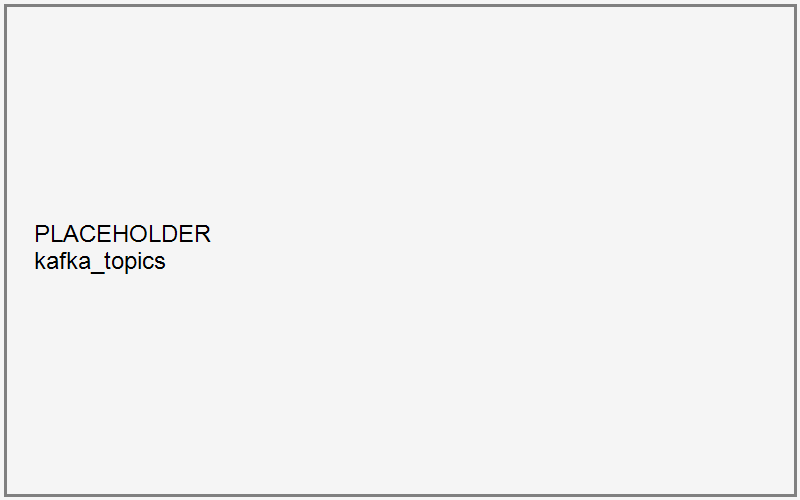
\includegraphics[width=13cm]{captures/kafka_topics.png}
    \caption{Capture d'écran — Gestion des sujets Kafka (portail client)}
    \label{fig:capture-kafka}
\end{figure}

\begin{figure}[h!]
 \centering
    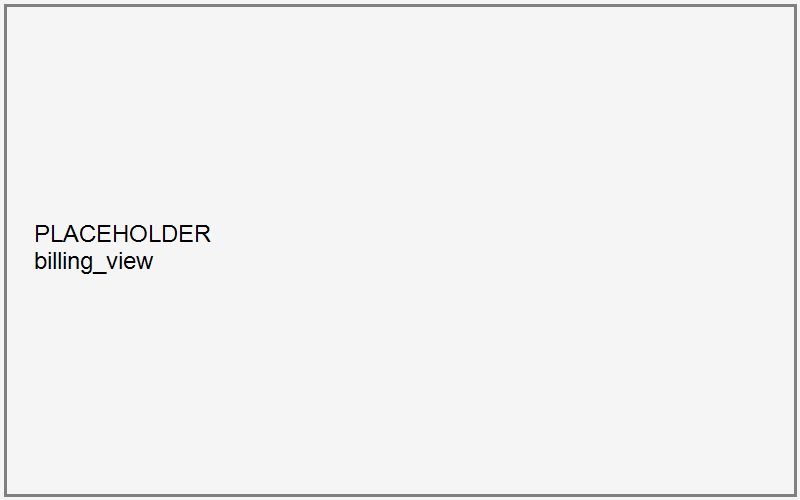
\includegraphics[width=13cm]{captures/billing_view.png}
    \caption{Capture d'écran — Facturation du compte client}
    \label{fig:capture-billing}
\end{figure}

\subsection{Difficultés rencontrées et solutions apportées}

\begin{itemize}
    \item \textbf{Simplification du périmètre de la console d'administration} : deux pages initialement prévues sur la console d'administration, dédiées à la gestion des incidents et à la détection d'anomalies (\texttt{AdminIncidents}, \texttt{AdminAnomalies}), ont finalement été retirées du menu de navigation afin de simplifier l'interface, la valeur ajoutée de ces vues étant jugée insuffisante par rapport à leur coût de maintenance à ce stade du projet. Il s'agit d'une décision de réduction de périmètre assumée, et non d'un abandon lié à une difficulté technique.
    \item \textbf{Décalage entre nom d'utilisateur et identifiant effectif dans les journaux affichés côté frontend} : une régression, apparue après la correction de l'isolation des journaux au Sprint 5, a conduit le frontend à transmettre le nom d'utilisateur plutôt que l'identifiant effectif attendu par le backend. \textit{Solution} : correction du frontend pour utiliser systématiquement l'identifiant effectif fourni par le contexte d'authentification.
\end{itemize}

\subsection{Résultat obtenu}

Au terme de ce sprint, l'ensemble des fonctionnalités backend développées depuis la Release 1 sont exposées et exploitables au travers des deux interfaces graphiques de la plateforme.

\subsection{Conclusion du Sprint}

Ce sprint achève le périmètre fonctionnel de l'interface utilisateur de la plateforme. Le sprint suivant se concentre sur l'industrialisation des chaînes d'intégration continue de l'ensemble des composants.


\section{Sprint 10 : Optimisation du pipeline CI/CD}

\subsection{Introduction}

Ce sprint a pour objectif de consolider et d'harmoniser les pipelines d'intégration continue des quatre composants de la plateforme (backend, portail client, console d'administration, et un pipeline distinct pour les microservices), en généralisant les mécanismes de fiabilisation mis au point empiriquement lors du Sprint 5 pour le pipeline backend.

\subsection{Objectifs du Sprint}

\begin{itemize}
    \item Harmoniser les quatre pipelines Jenkins existants sur un socle commun plus robuste.
    \item Fiabiliser l'exécution de Kaniko afin d'éviter les échecs de construction dus à la corruption de l'environnement Jenkins identifiée au Sprint 5.
    \item Clarifier l'usage des différents fichiers Dockerfile du backend, source de confusion identifiée lors de l'audit du projet.
\end{itemize}

\subsection{Sprint Backlog}

\begin{table}[!ht]
\begin{center}
     \begin{tabular}{|l{11cm}|l{3cm}|}
     \hline
     \textbf{User Story} & \textbf{Statut} \\
     \hline
     En tant qu'exploitant, je veux que les échecs de checkout Git soient automatiquement réessayés & Réalisé (backend uniquement) \\
     \hline
     En tant qu'exploitant, je veux que Kaniko ne corrompe plus l'environnement Jenkins & Réalisé (backend uniquement) \\
     \hline
     En tant qu'exploitant, je veux un pipeline unique et cohérent pour tous les composants & Non réalisé \\
     \hline
     En tant qu'exploitant, je veux une étape de tests automatisés dans les pipelines & Non réalisé \\
     \hline
     En tant qu'exploitant, je veux une analyse de sécurité des images construites & Non réalisé \\
     \hline
     \end{tabular}
     \caption{Sprint Backlog — Sprint 10}
     \label{tab:sb-sprint10}
     \end{center}
\end{table}

\subsection{Réalisation}

Les correctifs de fiabilisation identifiés au Sprint 5 (options Kaniko \texttt{--use-new-run}/\texttt{--snapshot-mode=redo}, redémarrage sécurisé systématique de Jenkins, réessai automatique du \textit{checkout} Git) demeurent, à l'issue de ce sprint, appliqués uniquement au pipeline du backend, qui reste le plus mature des quatre. Le remplacement du fichier \texttt{backend.Dockerfile} (construction multi-étapes avec utilisateur non privilégié, non utilisé en pratique par le pipeline) au profit exclusif de \texttt{backend-kaniko.Dockerfile} (construction mono-étape effectivement utilisée) a été clarifié dans la documentation technique du projet, sans toutefois que le premier fichier, devenu du code mort, n'ait été supprimé du dépôt.

\subsection{Difficultés rencontrées et limites assumées}

En toute rigueur, ce sprint doit être présenté avec honnêteté au regard de son objectif initial : \textbf{l'optimisation du pipeline CI/CD n'a été que partiellement atteinte}. Les difficultés suivantes, documentées par les audits menés sur la plateforme, n'ont pas été résolues dans le temps imparti du projet et sont reprises comme perspectives d'amélioration au chapitre de validation :

\begin{itemize}
    \item Les pipelines du portail client et de la console d'administration n'ont \textbf{pas} été alignés sur les mécanismes de fiabilisation du pipeline backend.
    \item Le pipeline dédié aux microservices reste le moins abouti des quatre : construction et publication d'image Docker classiques (sans Kaniko), absence d'identifiants explicites pour le \textit{checkout} Git, et absence de toute étape de déploiement Kubernetes final.
    \item Aucun des quatre pipelines ne comporte d'étape de tests automatisés (la compilation backend est réalisée avec l'option \texttt{-DskipTests}), d'analyse statique de code, ni d'analyse de vulnérabilités des images construites.
    \item Aucun mécanisme de \textit{rollback} automatique n'est déclenché en cas d'échec de la vérification du déploiement (\texttt{kubectl rollout status}).
\end{itemize}

Ces limites ne remettent pas en cause le fonctionnement de la plateforme, qui reste opérationnelle et déployée automatiquement à chaque évolution ; elles constituent en revanche des axes d'industrialisation identifiés mais non traités, dans un contexte de projet à ressources et délai contraints, où la priorité a été donnée à la robustesse fonctionnelle de la plateforme elle-même plutôt qu'à l'homogénéisation complète de ses quatre pipelines.

\subsection{Résultat obtenu}

Au terme de ce sprint, le pipeline backend demeure le plus robuste et le plus représentatif de la démarche CI/CD visée pour la plateforme ; les trois autres pipelines restent fonctionnels mais perfectibles, les limites identifiées étant explicitement documentées plutôt que dissimulées.

\subsection{Conclusion du Sprint}

Ce sprint clôt la Release 3. L'ensemble des composants de la plateforme (backend, deux frontends) sont désormais construits et déployés automatiquement, avec un niveau de maturité inégal selon le composant, honnêtement documenté. La Release suivante, consacrée à la validation, revient en détail sur l'ensemble de ces limites ainsi que sur les tests réalisés sur la plateforme dans son ensemble.

\section{Conclusion}

La Release 3 a rendu la plateforme pleinement utilisable par ses utilisateurs finaux, au travers de deux interfaces graphiques couvrant l'intégralité du périmètre fonctionnel développé depuis la Release 1, et a engagé un travail d'industrialisation des chaînes de déploiement continu. Ce travail d'industrialisation, présenté ici avec la même rigueur que les fonctionnalités abouties, n'a été que partiellement mené à son terme : ce constat, assumé, alimente directement le chapitre de validation qui clôt ce mémoire.

\chapter*{chapitre 7}
\markboth{Chapitre 7 }{7 Validation} %pour afficher l'entete
 \addcontentsline{toc}{chapter}{7 Validation}

\textbf{\Huge Validation}

\setcounter{chapter}{7}
\setcounter{section}{0}

\section{Introduction}

Les chapitres précédents ont présenté la réalisation progressive de la plateforme, release après release, en documentant au fil de l'eau les anomalies rencontrées et les corrections apportées. Ce chapitre, qui regroupe le Sprint 11 (tests, validation, corrections et stabilisation) et le Sprint 12 (documentation et préparation de la soutenance), a pour objectif de dresser un bilan global et honnête de l'état de la plateforme au terme du projet : la méthodologie de test suivie, les résultats obtenus, l'évolution de la posture de sécurité mesurée par deux audits successifs, et la synthèse consolidée des limites connues et des perspectives d'amélioration. Conformément à la démarche d'honnêteté académique adoptée tout au long de ce mémoire, ce chapitre ne cherche pas à masquer les points inachevés du projet mais à les documenter avec la même rigueur que les fonctionnalités abouties.


\section{Sprint 11 : Tests, validation, corrections et stabilisation}

\subsection{Introduction}

Ce sprint a pour objectif de valider, de manière transversale à l'ensemble des fonctionnalités développées depuis le Sprint 0, le comportement fonctionnel de la plateforme, et de mener un audit de sécurité formel destiné à identifier et corriger les vulnérabilités les plus critiques avant la mise en exploitation.

\subsection{Méthodologie de test}

La validation fonctionnelle de la plateforme s'est appuyée sur un plan de test manuel structuré, couvrant 84 cas de test répartis sur l'ensemble des modules fonctionnels de la plateforme (authentification et gestion des comptes, gestion des applications, gestion de Kafka, configuration de l'Eventing, facturation, supervision, administration). Ce plan de test constitue le référentiel méthodologique de la campagne de validation ; en toute rigueur, il convient de préciser qu'au moment de la rédaction de ce mémoire, ce document se présente comme une grille de vérification prête à l'exécution, dont les colonnes de statut restent à renseigner de manière exhaustive au fil de son exécution complète — il ne doit donc pas être présenté comme la preuve d'une campagne de test intégralement exécutée et tracée, mais comme la méthodologie de validation retenue pour le projet.

En complément de ce plan de test fonctionnel, la validation technique des fonctionnalités backend non encore exposées graphiquement au moment de leur développement (Kafka et Eventing, avant le Sprint 9) a été réalisée par appels directs à l'API REST à l'aide de l'outil Postman, comme indiqué au chapitre 2.

\subsection{Audit de sécurité et amélioration de la posture de sécurité}

Deux audits de sécurité successifs ont été menés sur la plateforme au cours de ce sprint, permettant de mesurer objectivement la progression de sa posture de sécurité.

Le premier audit a établi un score de sécurité initial de \textbf{4/10}, identifiant notamment les vulnérabilités suivantes, déjà évoquées au fil des chapitres précédents : accès non contrôlé à des ressources appartenant à d'autres tenants (IDOR) sur les journaux de déploiement et sur la suppression de moyens de paiement, secrets applicatifs versionnés en clair, configuration CORS trop permissive combinée à l'acceptation des identifiants de session, absence de limites de ressources par défaut sur les espaces de noms clients, rôles Kubernetes sous-déclarés, transmission du jeton d'authentification dans les paramètres d'URL du flux de journaux, absence de règles d'isolation réseau entre tenants, exécution du déploiement en apparence asynchrone mais en réalité bloquante, et incohérences du flux de journaux en temps réel selon le rôle de l'utilisateur.

Un second audit, mené après correction, a établi un score de \textbf{5{,}2/10}, sur la base du traitement suivant :

\begin{table}[!ht]
\begin{center}
     \begin{tabular}{|p{7cm}|l{5cm}|}
     \hline
     \textbf{Vulnérabilité identifiée} & \textbf{Traitement} \\
     \hline
     IDOR sur les journaux de déploiement & Corrigé \\
     \hline
     IDOR sur la suppression de moyens de paiement Stripe & Corrigé \\
     \hline
     Secrets en clair dans les manifestes versionnés & Corrigé (déplacés en \texttt{Secret} Kubernetes) \\
     \hline
     Configuration CORS permissive avec identifiants de session & Corrigé (liste blanche explicite) \\
     \hline
     Absence de limites de ressources par défaut par tenant & Accepté comme risque produit (modèle \og paiement à l'usage \fg) \\
     \hline
     Rôles Kubernetes (RBAC) sous-déclarés & Corrigé (reconstruits et vérifiés) \\
     \hline
     Jeton d'authentification transmis en paramètre d'URL (SSE) & Corrigé \\
     \hline
     Authentification par mot de passe direct (ROPC) au lieu d'Authorization Code + PKCE & Accepté comme risque produit \\
     \hline
     Absence de règles d'isolation réseau entre tenants & Corrigé (création automatique par tenant) \\
     \hline
     \end{tabular}
     \caption{Synthèse du traitement des vulnérabilités identifiées lors de l'audit de sécurité}
     \label{tab:audit-securite}
     \end{center}
\end{table}

Sept des neuf vulnérabilités critiques ou majeures identifiées ont ainsi été effectivement corrigées, et deux ont fait l'objet d'une décision explicite d'acceptation du risque plutôt que d'une correction, faute de compatibilité immédiate avec le modèle produit visé (facturation à l'usage sans plafond de ressources) ou avec les contraintes de délai du projet (migration du flux d'authentification). Cette distinction entre \og corrigé \fg{} et \og risque assumé \fg{} constitue, de notre point de vue, une démarche d'ingénierie plus rigoureuse qu'une simple liste de correctifs, car elle documente une décision consciente plutôt qu'un oubli.

\subsection{Résultat obtenu}

Au terme de ce sprint, la plateforme a fait l'objet d'une validation fonctionnelle méthodique et d'un durcissement de sécurité mesurable, avec une progression objectivée de 4/10 à 5{,}2/10. La plateforme est jugée stable pour une démonstration et une exploitation pilote, sous réserve des limites explicitement documentées dans la section suivante.

\subsection{Conclusion du Sprint}

Ce sprint a permis de transformer une plateforme fonctionnellement complète en une plateforme dont le niveau de qualité et de sécurité a été objectivement mesuré et amélioré, plutôt que simplement supposé satisfaisant.


\section{Sprint 12 : Documentation et préparation de la soutenance}

\subsection{Introduction}

Ce dernier sprint a pour objectif de consolider la documentation technique de la plateforme et de préparer sa présentation devant le jury.

\subsection{Réalisation}

L'ensemble des décisions techniques, anomalies identifiées et correctifs apportés tout au long du projet ont été consignés de manière détaillée dans une documentation technique versionnée avec le code (guide technique complet, fiches de correctifs individuelles, rapports d'audit), constituant la source principale de ce mémoire. Un plan de sauvegarde et de restauration de la base de données PostgreSQL et de l'index Elasticsearch a également été formalisé, avec une politique de rétention de sept sauvegardes quotidiennes et quatre sauvegardes hebdomadaires.

\subsection{Résultat obtenu}

La plateforme dispose, au terme de ce sprint, d'une documentation technique exhaustive et d'un mémoire retraçant fidèlement sa réalisation, ses choix d'architecture et ses limites, prêts à être présentés devant le jury.

\subsection{Conclusion du Sprint}

Ce sprint clôt la conduite du projet selon la planification Scrum définie au premier chapitre.


\section{Synthèse des limites et perspectives d'amélioration}

Cette section consolide, en un point unique, l'ensemble des limites identifiées au fil des chapitres de réalisation, ainsi que les fonctionnalités explicitement non implémentées à ce stade du projet.

\begin{table}[!ht]
\begin{center}
     \begin{tabular}{|p{6.5cm}|p{7cm}|}
     \hline
     \textbf{Limite ou fonctionnalité absente} & \textbf{Statut / perspective} \\
     \hline
     Infrastructure du cluster (nœuds, CNI, MetalLB, Kourier) et cluster Kafka Strimzi non versionnés en infrastructure-as-code & Provisionnés manuellement (Sprints 0 et 2) ; perspective : formalisation via Helm/Kustomize/GitOps \\
     \hline
     Absence de limites de ressources (\texttt{LimitRange}) par défaut par tenant & Risque produit assumé (modèle à l'usage) \\
     \hline
     Flux d'authentification ROPC au lieu d'Authorization Code + PKCE & Risque produit assumé \\
     \hline
     Absence d'isolation forte (SASL/mTLS/ACL) entre tenants sur le cluster Kafka partagé & Non implémenté ; perspective : \texttt{KafkaUser} par tenant avec ACL dédiées \\
     \hline
     Jeton et jeton de rafraîchissement stockés dans le stockage local du navigateur & Non corrigé ; perspective : migration vers un stockage plus sûr (cookie \textit{httpOnly}) \\
     \hline
     Collecte Prometheus des métriques du backend potentiellement toujours inopérante (étiquette de sélection incohérente) & Anomalie identifiée, correction non confirmée en production \\
     \hline
     Console d'administration exposée sur un port réseau fixe sans protection réseau dédiée & Non corrigé ; perspective : restriction d'accès réseau ou VPN dédié \\
     \hline
     Absence d'analyse de vulnérabilités des images de conteneurs dans les pipelines CI/CD & Non implémenté ; perspective : intégration d'un scanner d'images (ex. Trivy) \\
     \hline
     Conteneurs applicatifs exécutés avec l'utilisateur root par défaut & Non corrigé ; perspective : imposition d'utilisateurs non privilégiés \\
     \hline
     Pipelines CI/CD hétérogènes (portail, console, microservices moins aboutis que le backend) & Partiellement traité au Sprint 10 ; perspective : socle Jenkins commun \\
     \hline
     Absence de tests automatisés (unitaires/intégration) dans les pipelines CI/CD & Non implémenté ; perspective : intégration d'une étape de tests et de couverture de code \\
     \hline
     Duplication de code entre le portail client et la console d'administration & Non refactorisé ; perspective : extraction d'un paquet partagé ou passage à un monorepo \\
     \hline
     Mise en cache et découpage par domaine personnalisé (\textit{traffic splitting}, \textit{domain mapping}), non retrouvés dans le code audité & Non implémenté ; perspective d'évolution \\
     \hline
     \end{tabular}
     \caption{Synthèse des limites connues et des perspectives d'amélioration}
     \label{tab:limites}
     \end{center}
\end{table}

Cette synthèse illustre une caractéristique assumée de la démarche suivie tout au long du projet : privilégier, à ressources et délai constants, la robustesse fonctionnelle du parcours principal (déploiement, supervision, facturation) plutôt qu'une couverture exhaustive de toutes les dimensions non fonctionnelles souhaitables. Les limites identifiées ne remettent pas en cause la validité de la démonstration technique réalisée, mais constituent une feuille de route réaliste pour une éventuelle industrialisation ultérieure de la plateforme.


\section{Conclusion}

Ce chapitre a présenté la validation de la plateforme au travers d'une campagne de tests fonctionnels méthodique et d'un audit de sécurité en deux temps, ayant permis de mesurer objectivement une amélioration de la posture de sécurité du système. Il a également dressé la synthèse honnête des limites connues du projet, condition nécessaire, à notre sens, à la crédibilité scientifique et professionnelle de ce mémoire devant un jury de cycle ingénieur. La conclusion générale qui suit revient sur les apports globaux du projet au regard de la problématique posée au premier chapitre.

\include{Conclusion}

\bibliographystyle{alpha}
\bibliography{bibliography}
\addcontentsline{toc}{chapter}{Bibliographie}

\end{flushleft}

\pagestyle{empty}
%\include{Annexe1} % TODO: fichier d'annexe absent du dépôt, à créer si besoin

\include{garde_fin2}

\end{document}
